
\documentclass[conference]{IEEEtran}
\usepackage{cite}
\usepackage{amsmath}
\usepackage{placeins}
\usepackage{subfloat}
\usepackage{graphicx}
\usepackage[T1]{fontenc}
\usepackage[capitalise]{cleveref}
\usepackage{subcaption}
\hyphenation{op-tical net-works semi-conduc-tor}


\begin{document}
\title{Influence of Training Set Size on Generalization of Artificial Neural Network}
\author{
\IEEEauthorblockN{Hoang-Trieu TRINH}
\IEEEauthorblockA{Advanced Program in Computer Science\\Faculty of Information Technology
\\Ho Chi Minh University of Science\\
thtrieu@apcs.vn}
\and

\IEEEauthorblockN{Huu-Phat HO}
\IEEEauthorblockA{Advanced Program in Computer Science\\Faculty of Information Technology
\\Ho Chi Minh University of Science\\
hhphat@apcs.vn}
\and
\IEEEauthorblockN{Nhat-Thanh KIM}
\IEEEauthorblockA{Advanced Program in Computer Science\\Faculty of Information Technology
\\Ho Chi Minh University of Science
\\knthanh@apcs.vn}
}
\maketitle
\begin{abstract}
%\boldmath
Artificial Neural Networks have long been considered to be capable of solving a wide range of difficult problems. In addition, the available training data is also growing exponentially everyday thanks to a more open and globally connected information network. According to the conventional belief that more data should always refine the model's estimators, it is reasonable for one to be optimistic about future capability of neural networks. To verify this, the authors investigate the performance of different neural network architectures on MNIST database's test set (10k) after training them on different portions of the full training set (60k). The purpose of this experiment is to find out whether using the full training set is best in terms of the performance on test set. Result shows that for some architectures of neural network, the answer is negative. This casts doubt on situations where other classifiers are applied without any consideration of a partial usage from the corresponding training set. The result also implies that a new approach should be proposed while assessing the relative performance of different classifiers after being trained on the same data.
\end{abstract}

\begin{IEEEkeywords}
artificial neural network, MNIST, accuracy, generalization.	 

\end{IEEEkeywords}

\IEEEpeerreviewmaketitle

\section{Introduction}
\label{sec:introduction}
Inspired by biological neural networks, artificial neural networks are a group of probabilistic and statistical models designed to learn from a large amount of input in order to approximate unknown functions. Thanks to their flexible nature as universal approximators, neural networks have been able to solve a wide range of problems that are previously considered to be difficult in machine learning, computer vision, and speech recognition \cite{NovelConnectionist,Kurzweilinterview}. After a time being outran by new methods such as Support Vector Machines and Linear models, Neural Networks regain their popularity in early 2000s under the new name Deep Learning, thanks to new in-depth development on their architecture and advances in modern computer's computational capabilities \cite{NIPS2008_3449,Rumelhart:ExploMicroStructure}.

Mutually assistant to this growth is the astronomical amount of data that is still growing ever since the establishment of Internet and large data centers\cite{website:dataeverywhere}. Specifically, more data gives a richer source of training material, and more refined models are more accurate in making sense of new data. An epitome of the successful application of neural networks is the MNIST (Mixed National Institute of Standards and Technology) database of handwritten digits, which consists of 60,000 training images and 10,000 testing images, each is a 28x28 pixel gray scale image \cite{Kussul_improvedmethod}. The MNIST database is presented in a way that minimizes user's effort on preprocessing and formatting, therefore it is commonly used for practicing various machine learning and image processing techniques\cite{SVMSpeedPatternReg,usinganalytic}.

A number of scientific papers on different algorithms have been introduced in attempt to lower the state-of-the-art error rate on MNIST test set \cite{FastKNNClusterBasedTrees,MNISTHandWritten}. Some of these include additional preprocessing steps applied to the training set such as deskewing, noise removal, blurring, subsampling, or augmentation with distorted versions of the original training examples\cite{Lecun98gradient-basedlearning}. In 2012, a group of researchers built a committee of 35 Convolutional Neural Networks, trained on the width-normalized MNIST training set, achieved an accuracy of 0.23 percent \cite{MultiColummn}.

All of the existing classifiers implemented on MNIST dataset are trained on the complete training set, which consists of 60,000 handwritten digit patterns, or its augmented version\cite{Lecun98gradient-basedlearning}. However, it is reported that more training data does not guarantee a better estimation of the model's parameters in terms of their mean squared error \cite{IGotMoreData,WhenItSeem}. Practically speaking, this can be due to the fact that the training data is biased, or the given data distribution disagrees in relevant ways with some of the model assumptions \cite{WhenItSeem}. This experiment examines the validity of training a classifier on the complete MNIST training set and evaluate its performance on the complete MNIST test set.

To address this, the authors tested the performance of a number of neural network's architectures on the complete MNIST test set after training them on different subsets of the MNIST training set. The training subsets are arranged in an order such that the smaller one is a subset of the bigger one. This is to expose the changes in a particular algorithm's accuracy when adding more data to the resource it has already seen. Different neural network architectures with various capacities when tested on MNIST test set also shows the effect of adding more data into different models.

Result shows that the dominant trend when adding more data is an improvement of accuracy on the MNIST test set. For some sizes of hidden layer, however, 60,000 training examples does not give the best performance on MNIST test set. Interestingly, the worsening effect of adding more data on neural network's accuracy can be seen more clearly when these networks are trained on two subsets of size 30,000 and 40,000. At these points, there is a considerable number of neural networks that appear to have failed to improve their performance on MNIST test set. In fact, their accuracy significantly dropped off the increasing tendency previously made by smaller training subsets with sizes 10,000 and 20,000.

\cref{sec:background} introduces background and related works, \cref{sec:Experiment} shows the details of the experiment, \cref{sec:Result} reports our experiment's result and finally, \cref{sec:conclusion} sums up the authors' investigation and gives our final conclusion.
\section{Background and Related Work}
\label{sec:background}
\subsection{Main Concepts}
\paragraph{Perceptron}
First Artificial Neural Network invented in 1957 by F. Rosenblatt is Perceptron. Perceptron is a type of linear classifier that establishes its predictions based on a linear predictor function, which is a set of coefficients and explanatory variables, combining a set of weights with the feature vector to make a prediction\cite{perceptron}.
The model of Perceptron classifier:\[f(x) = sign({w^T}x + b)\]
The update rule: \[{w_j} = {w_j} + \alpha \left( {{f_i} - {y_i}} \right){x_{ij}}\] 
Unfortunately, Perceptron could not be trained to recognize many classes of patterns. Furthermore, Perceptron learning algorithm does not terminate if the learning set is not linearly separable.
\paragraph{Multilayer Perceptron}
\begin{figure}[tmbh]
\centering
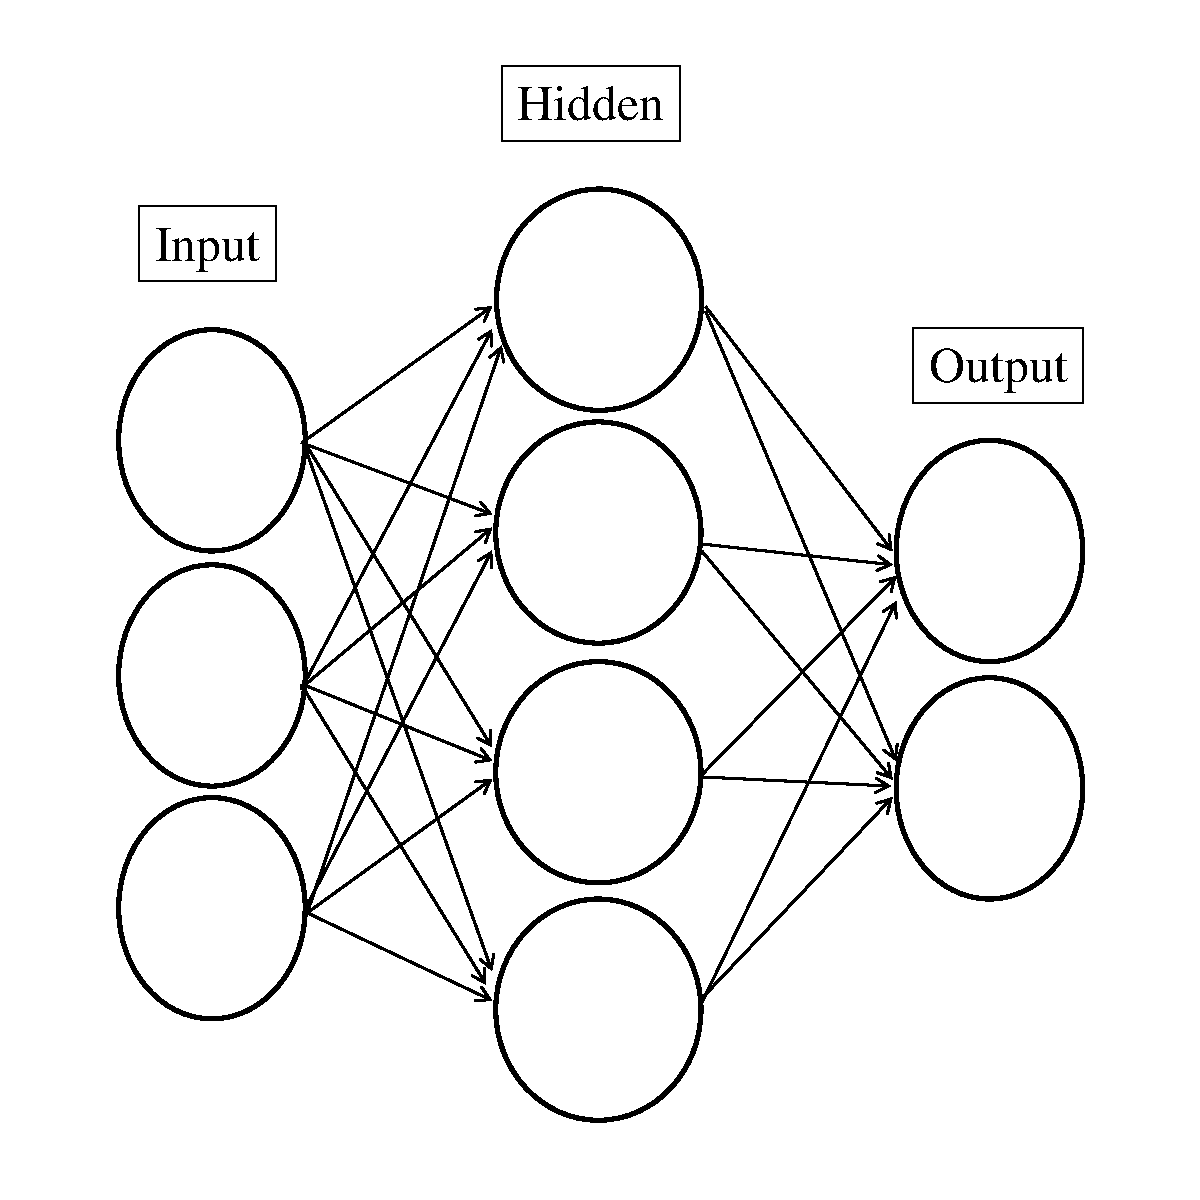
\includegraphics[width=7cm,height = 6cm]{mlp.pdf}
\caption{Multilayer Perceptron}
\label{figure:MLP}
\end{figure}
Because of the above limitations of Perceptron, researchers in this field came up with Multilayer Perceptron (MLP). As illustrated in \cref{figure:MLP}, MLP is a feed forward neural network that consists of three or more layers of nodes and each layer is fully connected to the next one\cite{Aizenberg07multilayerfeedforward}. If MLP has linear activate function, it can be proved that any number of layers can be reduced to the standard two-layer input-output model (Perceptron). Except for the activate function of output units, MLP uses sigmoidal/rectifier function instead of heavy-side as in Perceptron and is trained using back propagation\cite{CybenkoApproxSidmoid}. MLP is capable of both classification and regression. It also can distinguish non-linear separable data.
\paragraph{Artificial Neural Networks} 
Examinations of the human's brain system inspired the concept of Artificial Neural Networks (ANN). In ANN, simple artificial nodes, known as neurons, are connected together to construct a network. In detail, the structure of basic neural network includes many layers: input layer, hidden layer, output layer. Layers includes sets of interconnected nodes. Patterns are shifted through the network starting from the input layer. Specifically, the input layer communicates this information to hidden layers where the data is processed by a system of weighted connections. The hidden layers then transmit this processed information to the output layer\cite{FundermentalANN}. Due to the fact that ANNs have a powerful pattern classification and pattern recognition capability, the main function of this network is to forecast and estimate values from inputs by approximating functions\cite{ZhangANNForecast}. Application-wise, neural networks help improve solutions in hand writing recognition, which is known as the ability of a computer or a machine to receive and interpret apprehensible handwritten input from outside sources\cite{pittman2008handwriting}.   
\paragraph{Back-Propagation Neural Networks}
Although there are many different categories of learning rules for training Artificial Neural Networks on supervised-learning tasks, the authors concern only with traditional gradient-based methods\cite{buscema1998back}. These methods are made possible in the case of Neural Network thanks to the introduction of back-propagation (BP), an abbreviation for "backward propagation of errors". BP is an algorithm that helps compute the loss function's gradient with respect to each weight in the network. These gradients is evaluated recursively, starting from the gradient of output units and then propagate this information backward by chain rule. Suppose the forward flow of information is:
\[{z_j} = g\left( {a_j} \right)\]
\[{a_k} = \sum\limits_j {{w_{kj}}} {z_j}\]
Where $g()$ is the activation function and is required to be differentiable, ${w_{kj}}$ is the weight of the connection that sends information from unit $j$ to unit $k$. After that, the propagation process happens as follows:
\[{\Delta _j} = g'({a_j})\sum\limits_k {{w_{kj}}} {\Delta _k}\]
Where ${\Delta _i}$ is the gradient with respect to unit $i$. Unfortunately, BP have some drawbacks. After defining the general construction of a network and initially seeding the network with some random numbers, there is no other complicated work to do except feeding the network input, watching it trains, and waiting for the output. Another disadvantage of BPs is that it is likely to be slower to train than the others. Therefore, many techniques have been presented to deal with these problems\cite{Leonard1990337ImproveBPNN, Magoulas:1999:ImproveConvergenceBP, Riedmiller93adirect}.
\paragraph{Nonlinear conjugate gradient method using Polack-Ribiere formula}
Nonlinear conjugate gradient is a method to generalize the conjugate gradient method to nonlinear optimization. They use relatively little memory for large-scale problems and require no numerical linear algebra, but they typically converge much more slowly than Newton or quasi Newton methods\cite{dennis1977quasi}. The authors use Polak-Ribiere function to compute search directions and perform a line search using quadratic and cubic polynomial approximations\cite{grippo1997globally}. The Wolfe-Powells stopping-criteria is used together with the slope ratio method for guessing initial step sizes\cite{wei2000new}.
\paragraph{MNIST Database}
MNIST is one of most popular examples of the successful application of ANN. The MNIST database is a remixed subset of the NIST database, specifically a half of MNIST training set and a half of MNIST test set are taken from NIST training set, the other halves are taken from NIST test set\cite{FastKNNClusterBasedTrees}. This mixing is motivated by the fact that NIST training set and test set are taken from two different sources: The American Census Bureau employees and American high school students\cite{MNISTHandWritten}. Among different classifiers that are proposed by the MNIST database's original creators, a Support Vector Machine with polynomial kernel of degree 9 achieves an error rate of 0.8 percent, the only better one is a Convolutional Neural Network, which achieves an error rate of 0.7 percent\cite{Lecun98gradient-basedlearning}.
\paragraph{The Bias-Variance Trade-Off}
In supervised learning, when the model is being too simple and it could not fit the data and predict new data points accurately. The simpler model is called to have a high bias. On the other hand, when the model has too many parameters and fits almost all the data points but has poor prediction of new data points. The model is said to have high variance. The bias-variance trade-off is an acknowledged problem in machine learning and it usually occurs when we have relatively few data points or model becomes excessively complex \cite{Geman:1992:NNBBiasDilemma, BiasVarianceDecomposition}. A learning algorithm that reduces the chance of fitting noise and has good generalization is called robust.	
\subsection{Related Work}
Herman Chernoff investigates a two sample test originated from a satellite based experiment, which is designed to measure the Doppler effect in the relative motion of two astronomical objects. The experiment counts the number of photon emitted from both objects within a narrow energy band, during specified time interval \cite{WhenItSeem}. The test consists of data from Poisson counts and raises some puzzling questions due to the fact that its designer allocated relatively short time interval for each counts, hence there are some energy band with very small or zero counts. Herman Chernoff addresses the question of why ignoring data from these short time, low count intervals is desirable\cite{WhenItSeem}.

Xie and Meng observe samples generated from the heteroscedastic regression model ${Y_t} = \beta {X_t} + {\epsilon_t}$ (where ${\epsilon_t}~ N(0,{X_t}^2)$) independently and ${X_t}={(101-t)^{-1}}$ to conclude that the ordinary least squares estimator of $\beta$, despite being consistent, experiences an inflating variance when adding more data to the estimation procedure\cite{IGotMoreData}, this worsen $\beta$ in terms of its Mean Squared Error. The same effect happens to the simplest ARCH regression model with a single predictor ( ${Y_t}|{F_{t-1}}~N({X_t}\beta,{\tau_t}^2)$, where $t=1,\ldots,T$ and ${F_{t - 1}}$ is the $\sigma$-field generated by $\{{Y_1},\ldots,{Y_{t-1}}\}$ )\cite{IGotMoreData}. Meng proposes the concept of a statistical estimation procedure being self-efficient\cite{Meng94}. Intuitively, a self-efficient estimator cannot be improved by linearly combining itself with its bootstrapped version\cite{IGotMoreData}. Xie and Meng's work also conclude that additional data are not always helpful unless probabilistically principled methods such as Maximum Likelihood Estimation and Bayesian approaches are used\cite{IGotMoreData}.
\section{Experiment}
\label{sec:Experiment}

\subsection{The Classifier}
Since a one-hidden layer neural network is proven to have the universal approximation property\cite{Hornik_Universal_appro}, the authors restrict themselves only to single hidden layer and fully-connected sigmoidal neural networks. Each with one input layer of size 28 x 28 = 784, one output layer of size 10 corresponds to 10 number digits.

Specifically, there are 24 neural networks, which have respectively 20-, 40-, 60-, $\ldots$, 480-neuron in hidden layer. This range of hidden layer size is a natural choice in terms of completeness. It ensures the anticipated transition of accuracy on MNIST test set when each neural network goes from underfitting to overfitting its corresponding training set can be clearly observed. By this, the authors also examine how the influence of different training set sizes on neural network's performance differs across the 24 architectures.
\subsection{The database}
Neural networks are reportedly the best model to perform on MNIST database. This database's cleanliness in terms of handling and the abundant existing works are also among the authors' motivations of choosing this dataset.
\subsection{Training Sets}
The authors generate six training subsets from the complete MNIST training set using the following procedure:
\begin{enumerate}
\item Randomly sample 10,000 images from the complete MNIST training set to form the smallest training subset.
\item Exclude the previously sampled 10,000 training examples from the current MNIST training set.
\item Randomly sample another 10,000 images from the current MNIST training set and add them to the most recently created subset to form the next bigger one.
\item Repeat the procedure from its second step until the sixth subset is created, this last training set is also the complete MNIST training set.
\end{enumerate}
By including the full set of 60,000 training images into this experiment, the authors test the conventional anticipation that each of the classifiers would perform best when they are trained on this full dataset.
\subsection{Training Procedure}
24 neural networks are trained on the above 6 training sets with squared loss criterion and back-propagation in full-batch setting. Since this dataset is relatively small, the update rule is the nonlinear conjugate gradient rule with Polak-Ribiere version \cite{grippo1997globally}:
\begin{enumerate}
\item Calculate the steepest direction: \[\Delta {x_n} =  - {\nabla _x}f({x_n})\] 
\item Compute \({\beta _n}\) according to Polak-Ribiere formula\cite{Polak1969}. 
\item Update the conjugate direction: \[{s_n} = \Delta {x_n} + {\beta _n}{s_{n - 1}}\]
\item Perform a line search: \[{\alpha _n} = \mathop {\arg \min }\limits_\alpha  f({x_n} + \alpha {s_n})\]
\item Update the position: \[{x_{n + 1}} = {x_n} + {\alpha _n}{s_n}\]
\end{enumerate}
The script used is $fmincg$, developed and freely provided by Carl Edward Rasmussen. 

The quantities that this experiment aims at is the generalization rate \({G_χ}({\theta _{ij}})\) of these 24 neural networks after being trained on the six training subset:
\[{G_ \chi }({\theta _{ij}}) = \int\limits_ \chi  {L(f(} {\theta _{ij}},x ),C(x)){P_\chi }(x)dx\]
where \({\theta _{ij}}\) is the weight vector of neural network i after being trained on training subset $j$, \(f({\theta _{ij}}, \cdot )\) is the function represented by neural network with weight \({\theta _{ij}}\), $C(x)$ is the true class identity of $x$, and \({P_\chi}( \cdot )\) is the probability density function of input population $\chi$. Since the population is unavailable, \({G_\chi }\) is approximated unbiasedly by replacing the population $\chi$ by the test set \(\chi test\), \({P_\chi }\) is replaced by the empirical density function $F$, which puts equal mass on every point in its domain. 
\[{\widehat G_{\chi test}}({\theta _{ij}}) = \int\limits_{\chi test} {L(f(} {\theta _{ij}},x),C(x))F(x)dx\]
Thus, the quantities that we are to evaluate is  \({\widehat G_{\chi test}}(\widehat {{\theta _{ij}}})\) where \(\widehat {{\theta _{ij}}}\) is obtained by train on \(\chi train\):
\[\widehat {{\theta _{ij}}} = \arg {\max _{{\theta _{ij}}}}{\widehat G_{\chi train}}({\theta _{ij}})\]
Due to the non-linear nature of the cost function, it is impossible for heuristic algorithms such as gradient based methods to guarantee convergence at the global minimum \(\widehat {{\theta _{ij}}}\). For this reason, 
\(\widehat {{\theta _{ij}}}\) is in turn approximated by \(\widehat {\theta _{ij}^*}\):
\[\widehat {\theta _{ij}^*} = \mathop {\arg \min }\limits_{\widehat {\theta _{ij}^k},k = 1...K} {{\hat G}_{\chi train}}(\hat \theta _{ij}^k)\]
where
\[\widehat \theta _{ij}^k = fmincg(\theta _{ij}^k)\]
Specifically, each network is trained K times (the authors opt for K=3), starting with K different configurations for its initial set of weights to avoid early convergence due to shallow local minima. The initial weight vectors \(\theta _{ij}^k\) are generated by uniformly sampling from \({[0,1]^\Theta }\) (\(\Theta \) is the dimension of the weight vector). Each training stops when no more progress can be made by the algorithm due to convergence at a minimum, or numerically so close to a minimum to the extent that the current weight vector is technically indistinguishable to the optimal one. Among the three trained weight settings for each of 24 architectures, the one with best accuracy on MNIST training set is chosen to represent.
\section{Result}
\label{sec:Result}
\begin{table*}[tmbh]
\raggedright
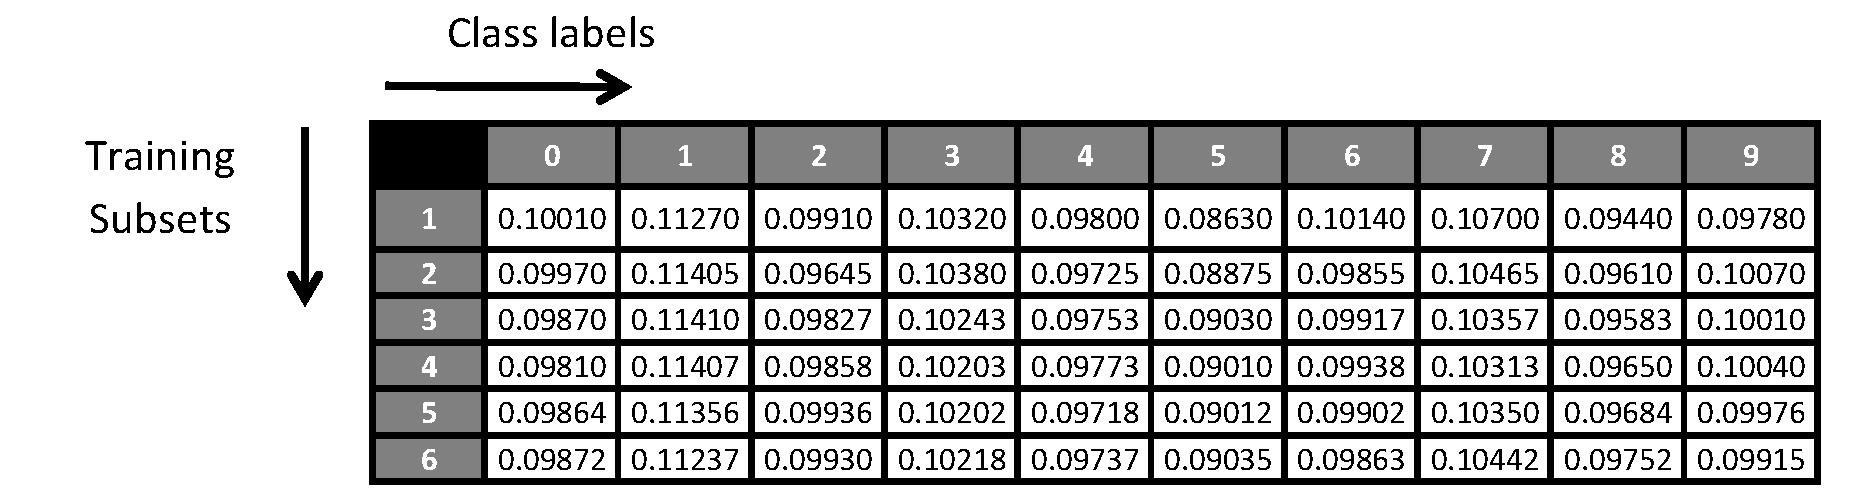
\includegraphics[width=17cm,height= 4.5cm]{ClassProportionVsTrainingSet.pdf}
\caption{Class Proportion vs. Training Set} 
\label{table:ClassProportionVsTrainingSet}
\end{table*}
\begin{figure}[tmbh]
\centering
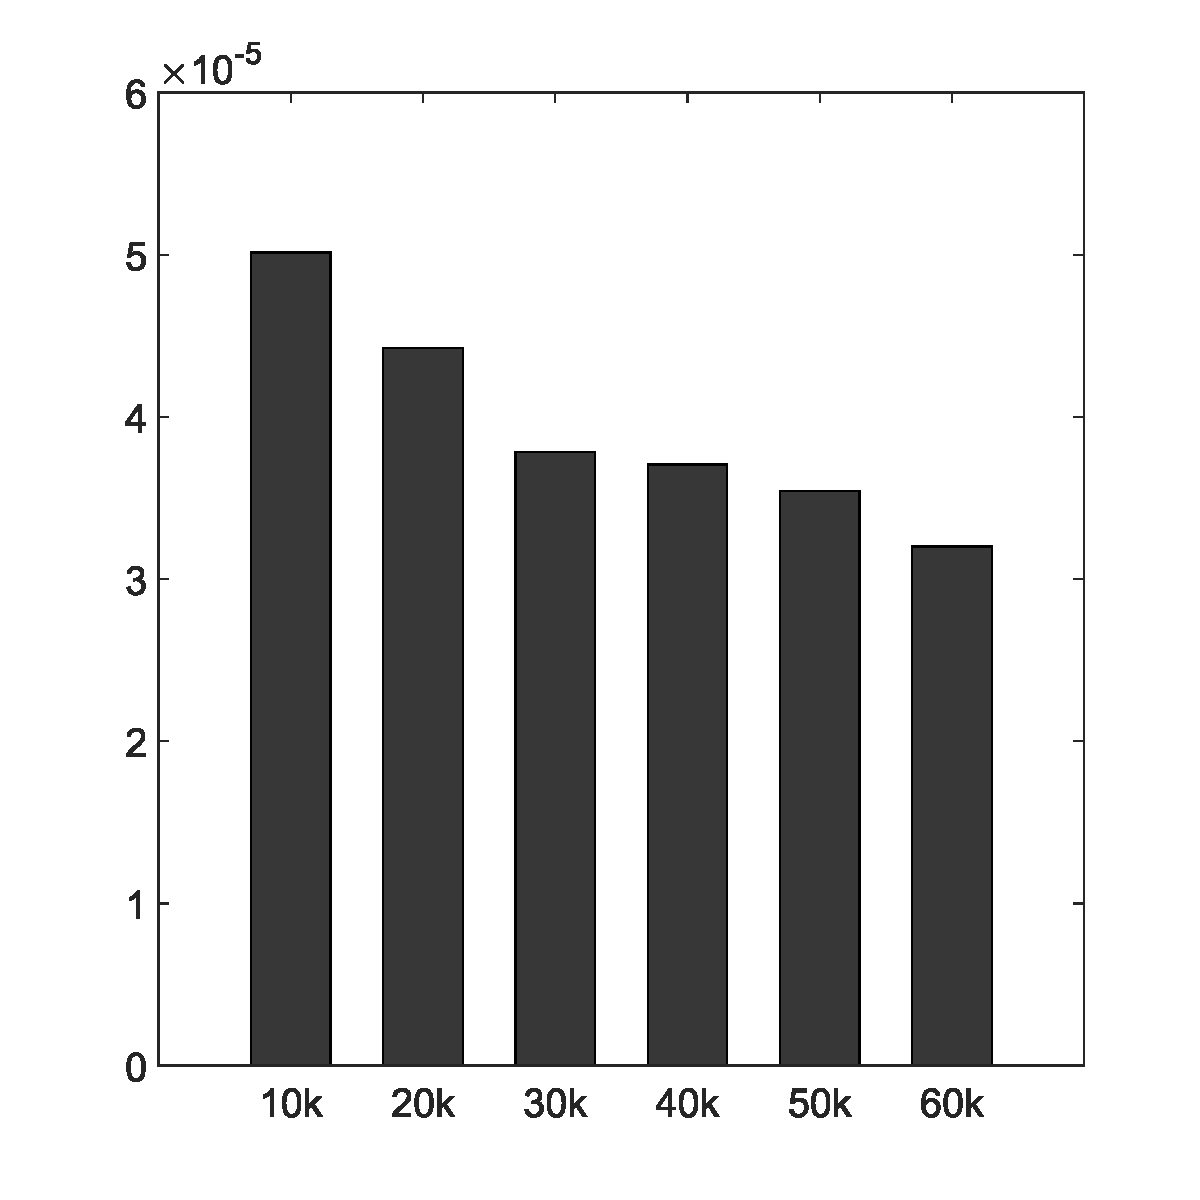
\includegraphics[width=8cm]{ClassProportionVarianceVsTrainingSet.pdf}
\caption{Class Proportion Variance vs. Training Set}
\label{figure:ClassProportionVarianceVsTrainingSet}
\end{figure}
\begin{subfigures}
\begin{figure}[tmbh]
\centering
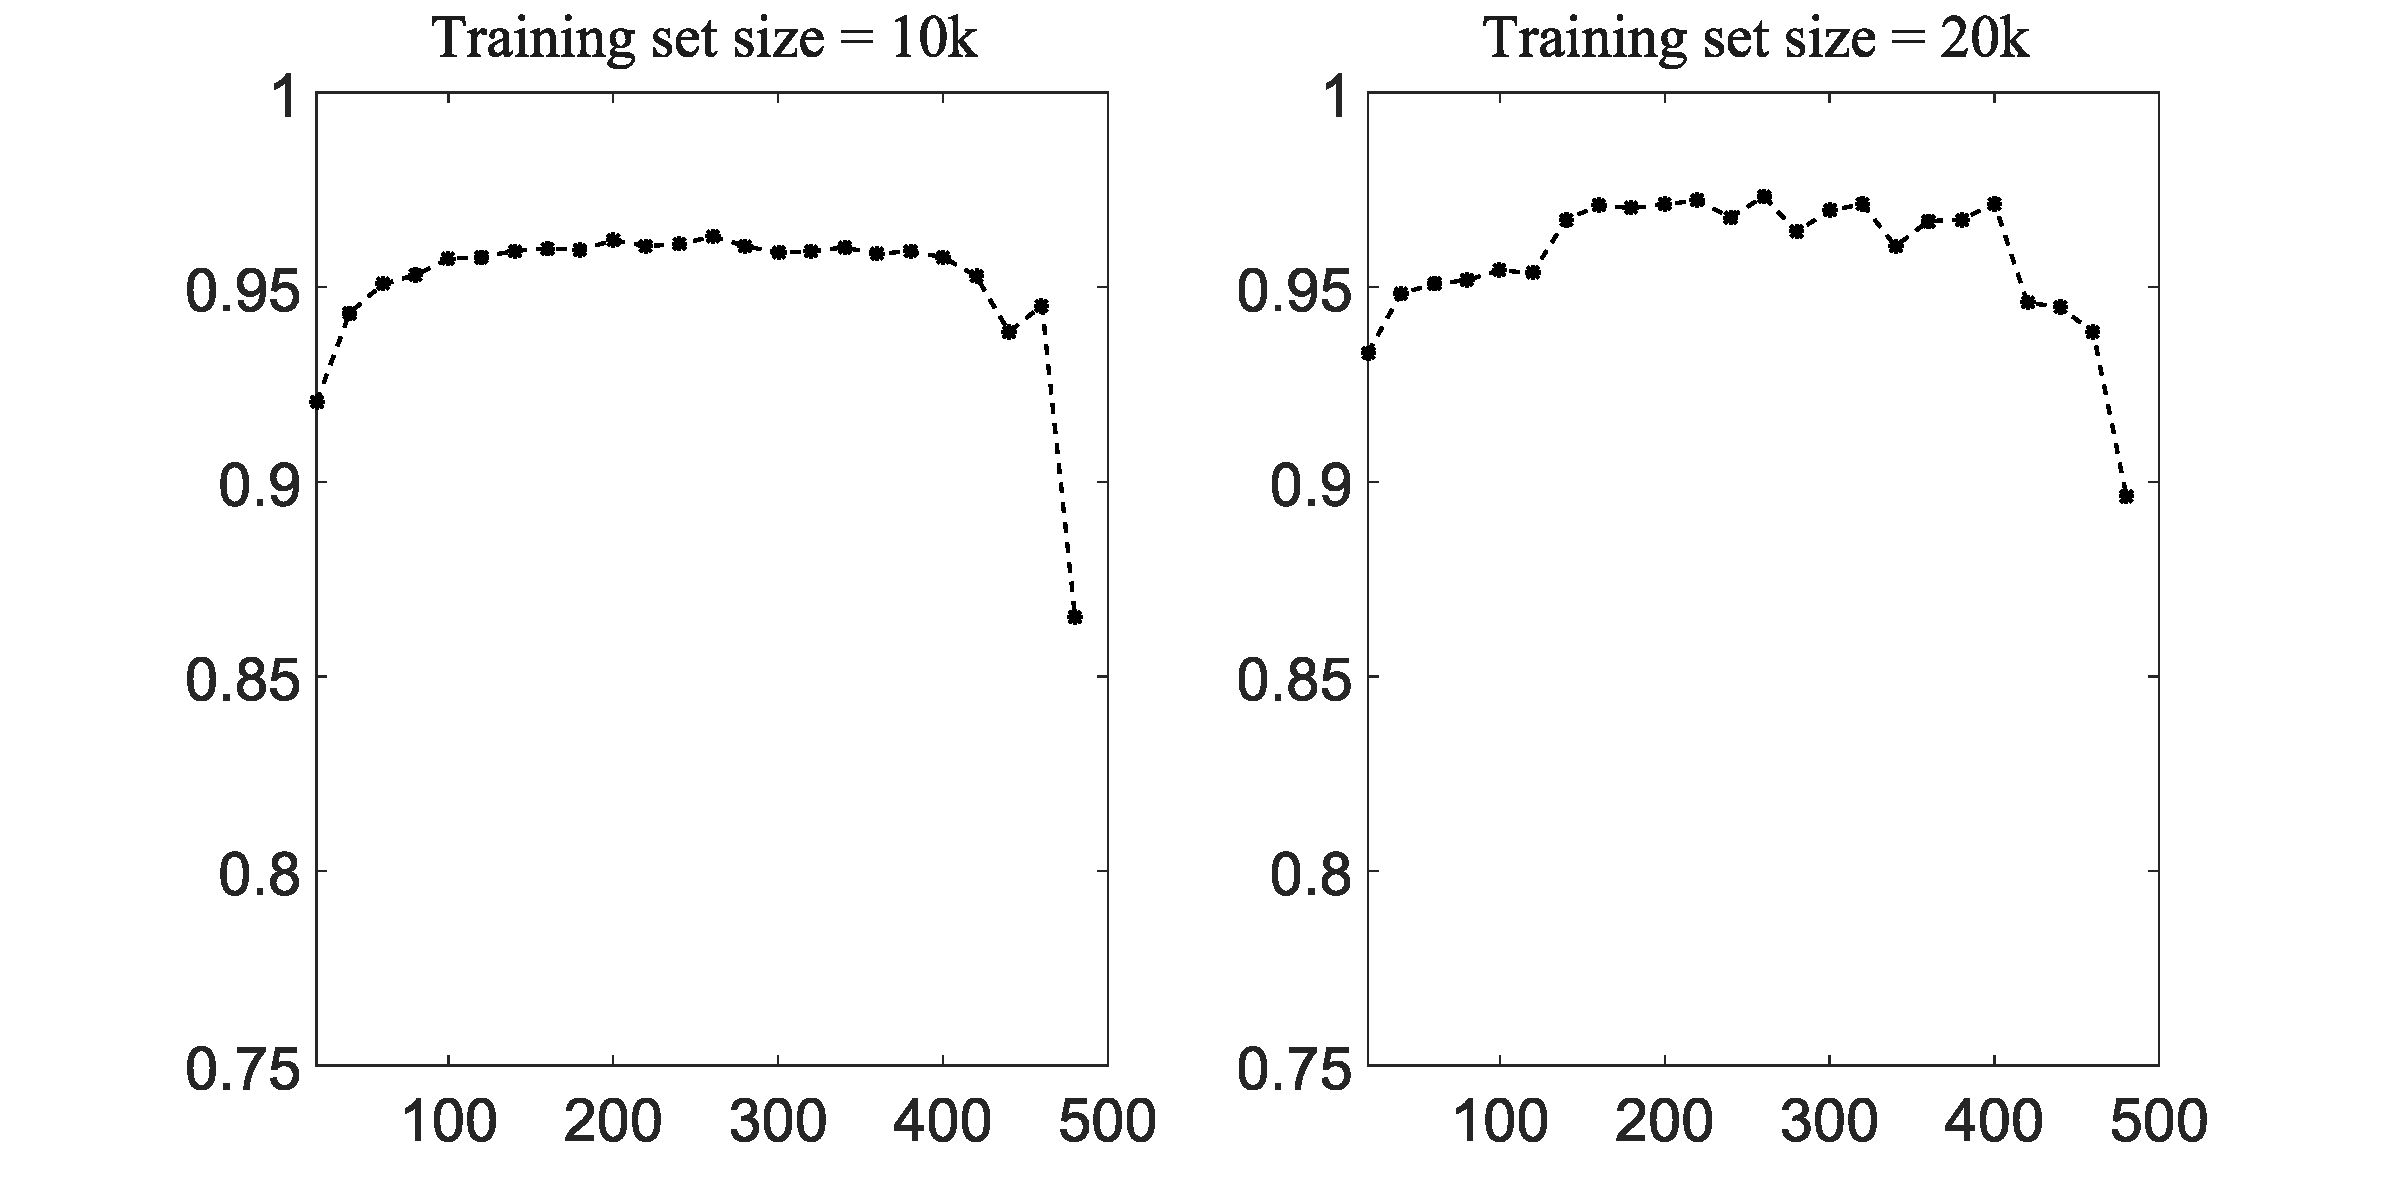
\includegraphics[width=10cm]{AccuracyHLSizeA.pdf}
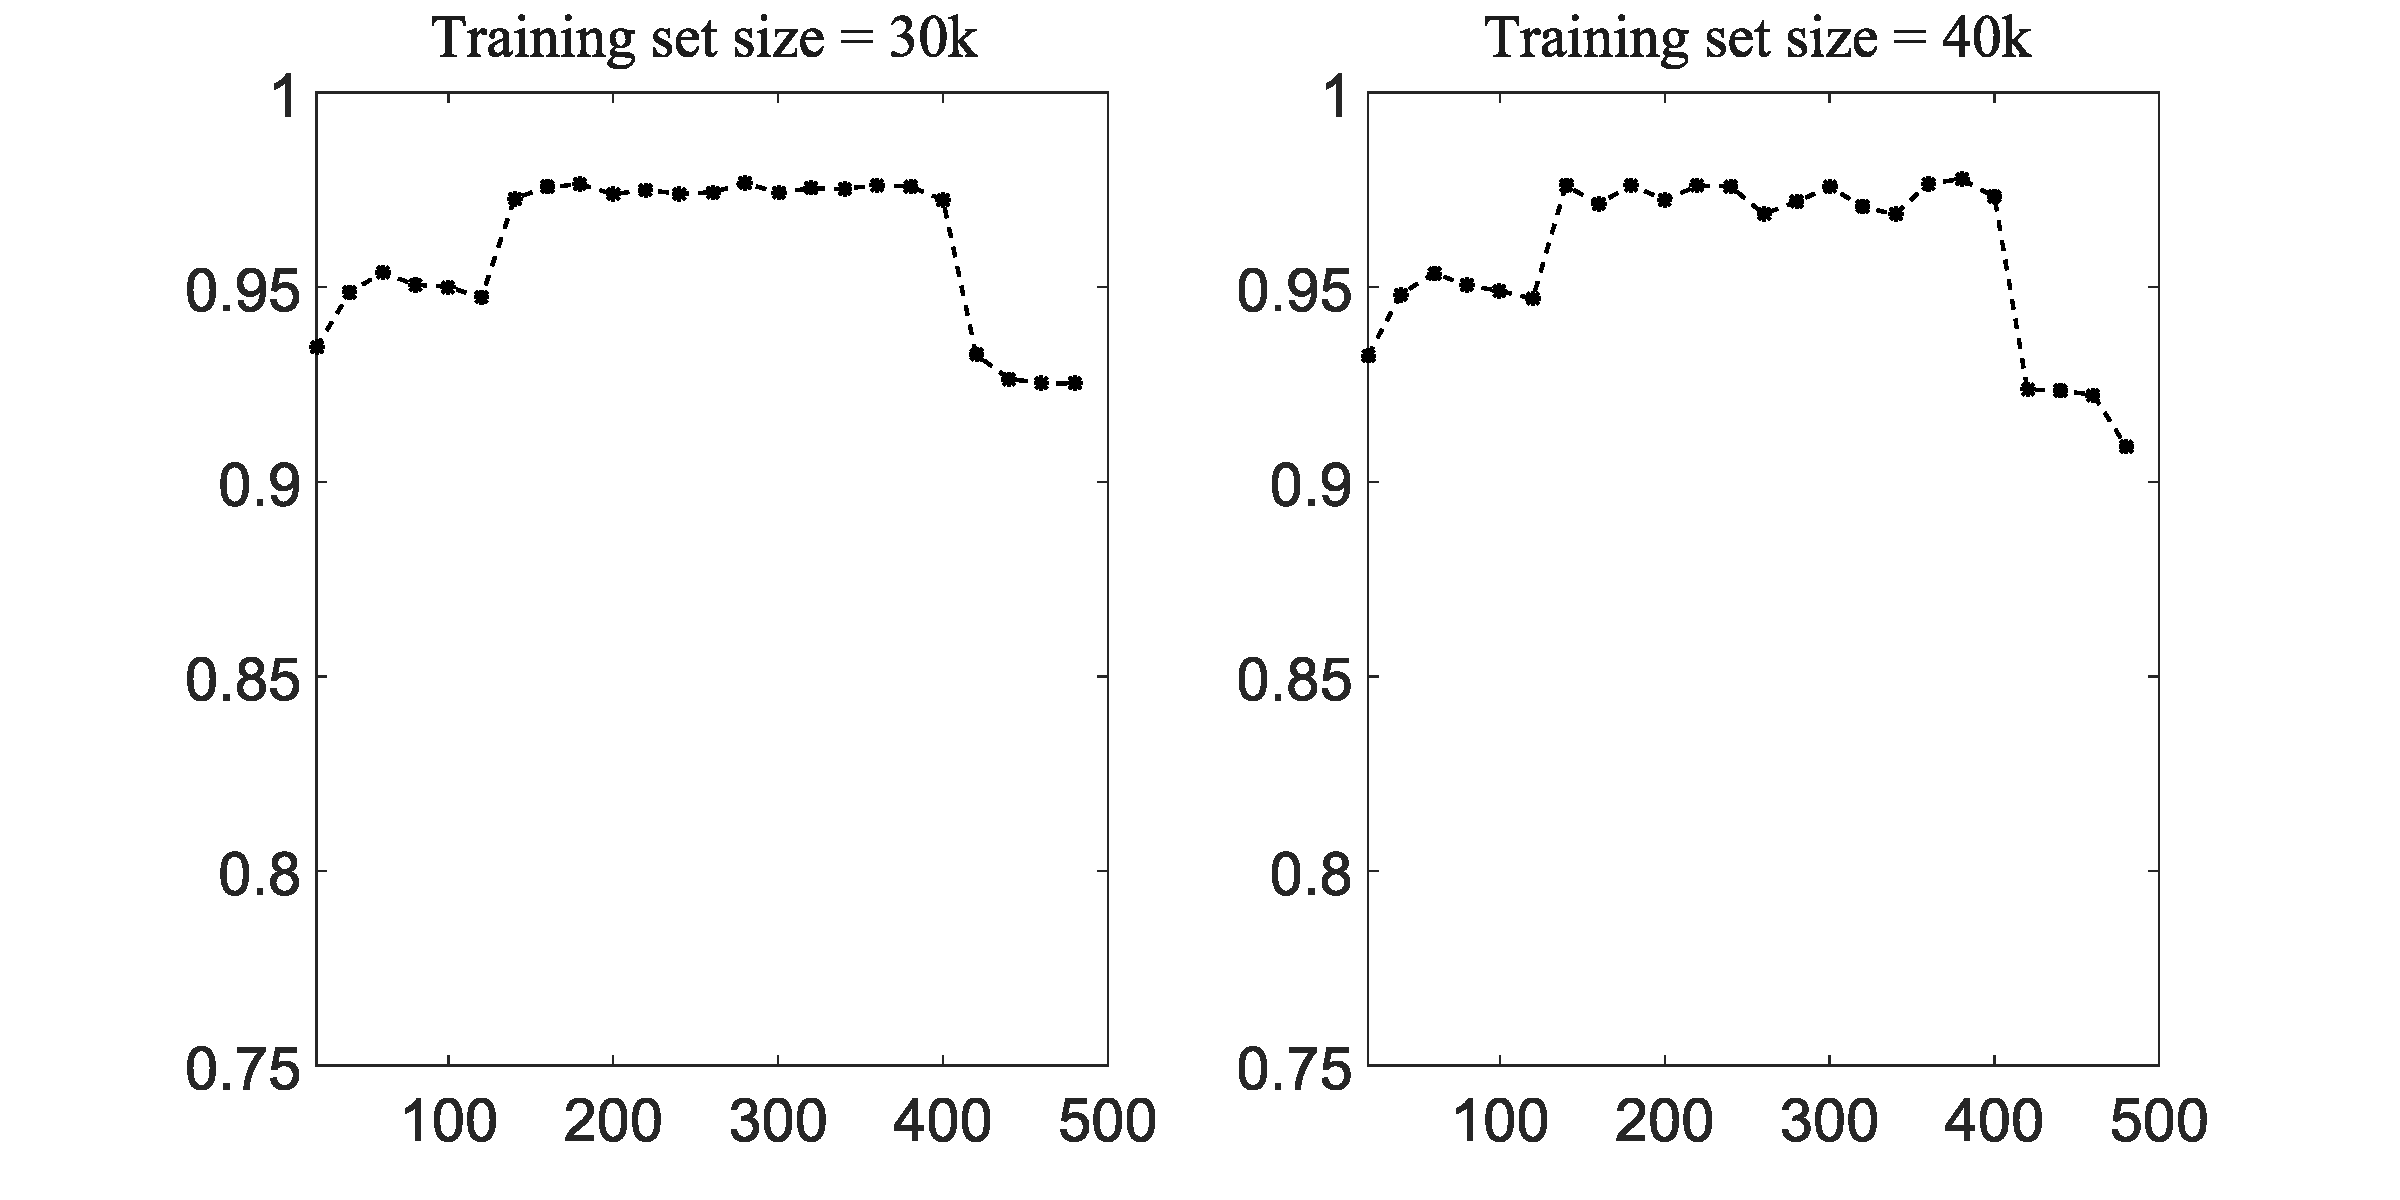
\includegraphics[width=10cm]{AccuracyHLSizeB.pdf}
\caption{Accuracy vs. Hidden layer size}
\label{figure:AccuracyHLSizeA}
\end{figure}
\begin{figure}[tmbh]
\centering
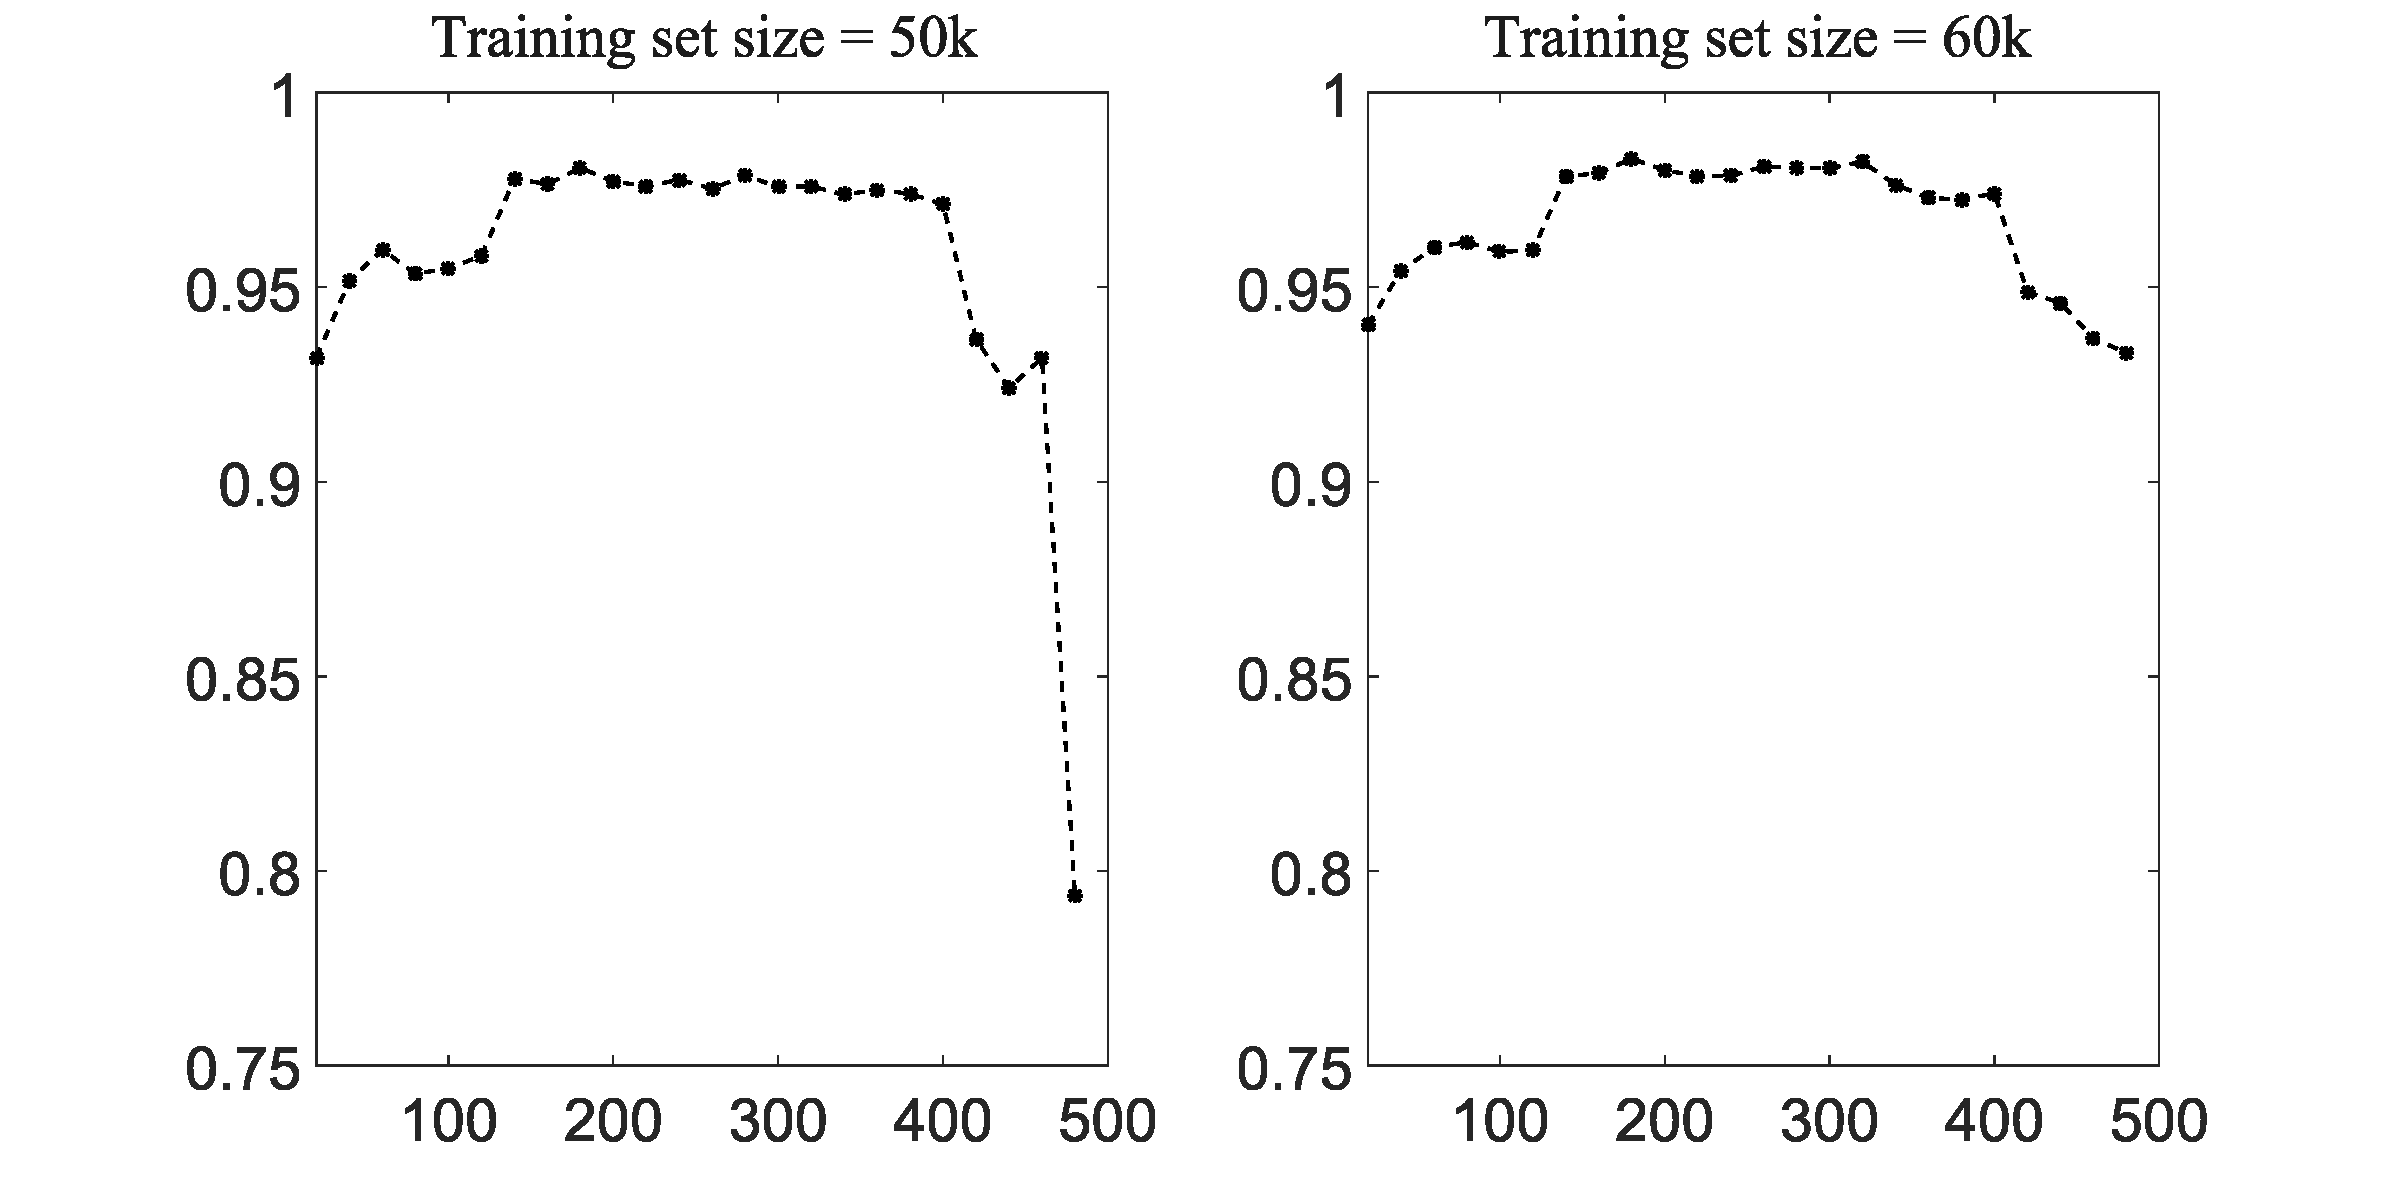
\includegraphics[width=10cm]{AccuracyHLSizeC.pdf}
\caption{Accuracy vs. Hidden layer size}
\label{figure:AccuracyHLSizeB}
\end{figure}
\end{subfigures}
\begin{figure}[tmbh]
\centering
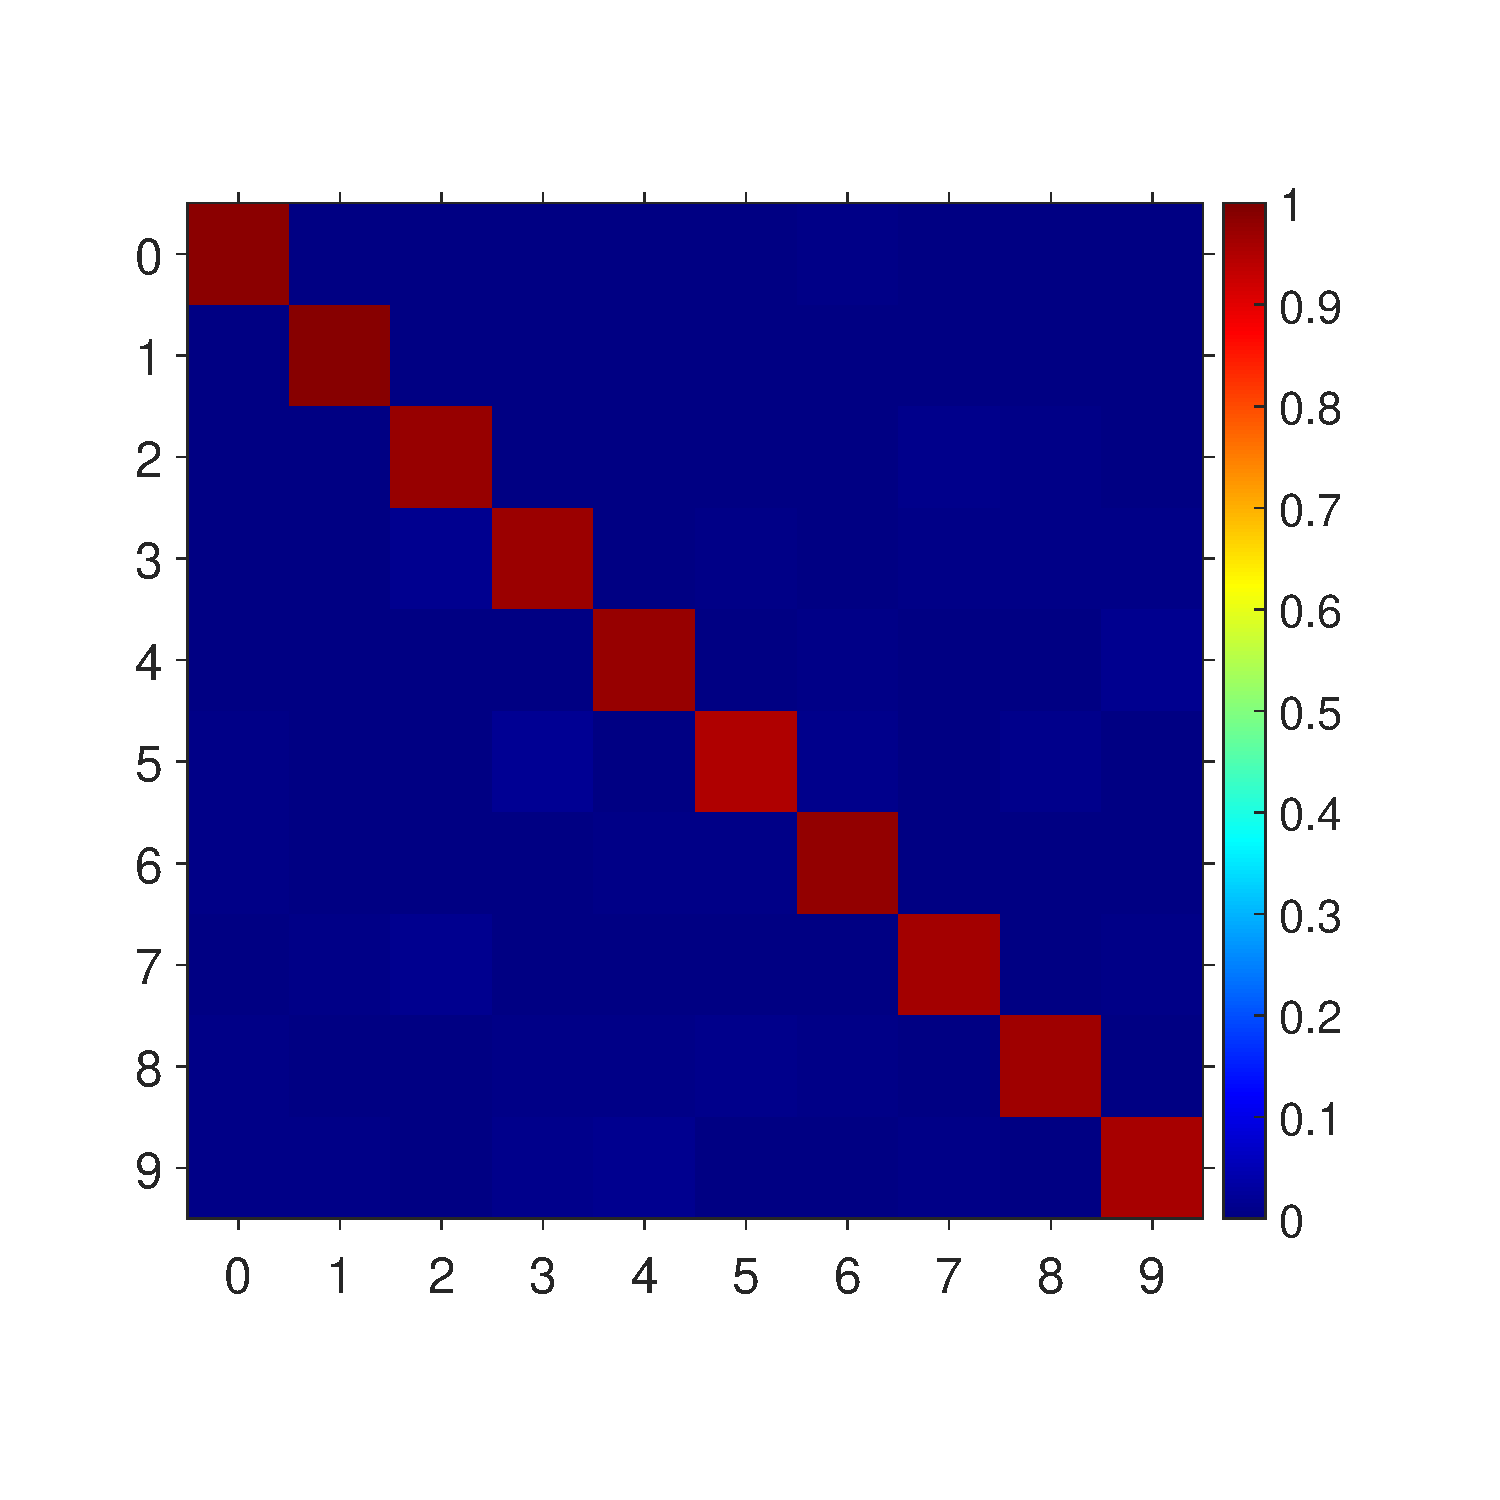
\includegraphics[width=8cm]{MatrixConfusion.pdf}
\caption{Confusion matrix}
\label{figure:MatrixConfusion}
\end{figure}
\begin{figure}[tmbh]
\begin{subfigure}{.23\textwidth}
  \centering
  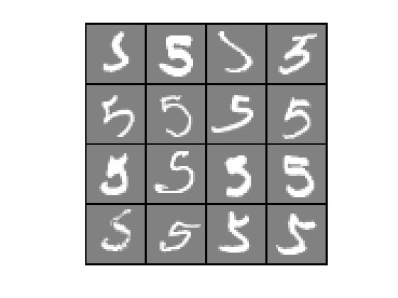
\includegraphics[width=.8\linewidth]{53.jpg}
  \caption{5 classified as 3}
\end{subfigure}%
\begin{subfigure}{.23\textwidth}
  \centering
  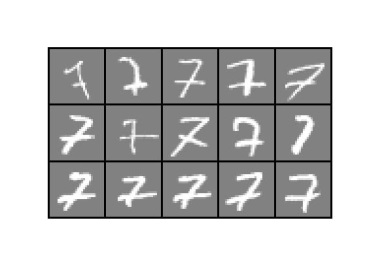
\includegraphics[width=.8\linewidth]{72.jpg}
  \caption{7 classified as 2}
\end{subfigure}
\begin{subfigure}{.23\textwidth}
  \centering
  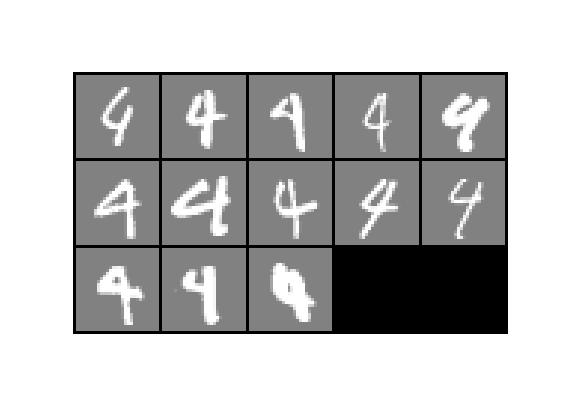
\includegraphics[width=.8\linewidth]{49.jpg}
  \caption{4 classified as 9}
  \end{subfigure}%
\begin{subfigure}{.23\textwidth}
  \centering
  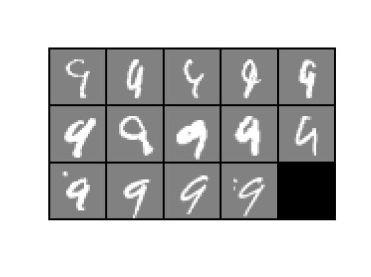
\includegraphics[width=.8\linewidth]{94.jpg}
  \caption{9 classified as 4}
 \end{subfigure}
 \caption{Most common confusions}
\label{figure:SomeConfusion}
\end{figure} 
\begin{subfigures}
\begin{figure}[tmbh]
\centering
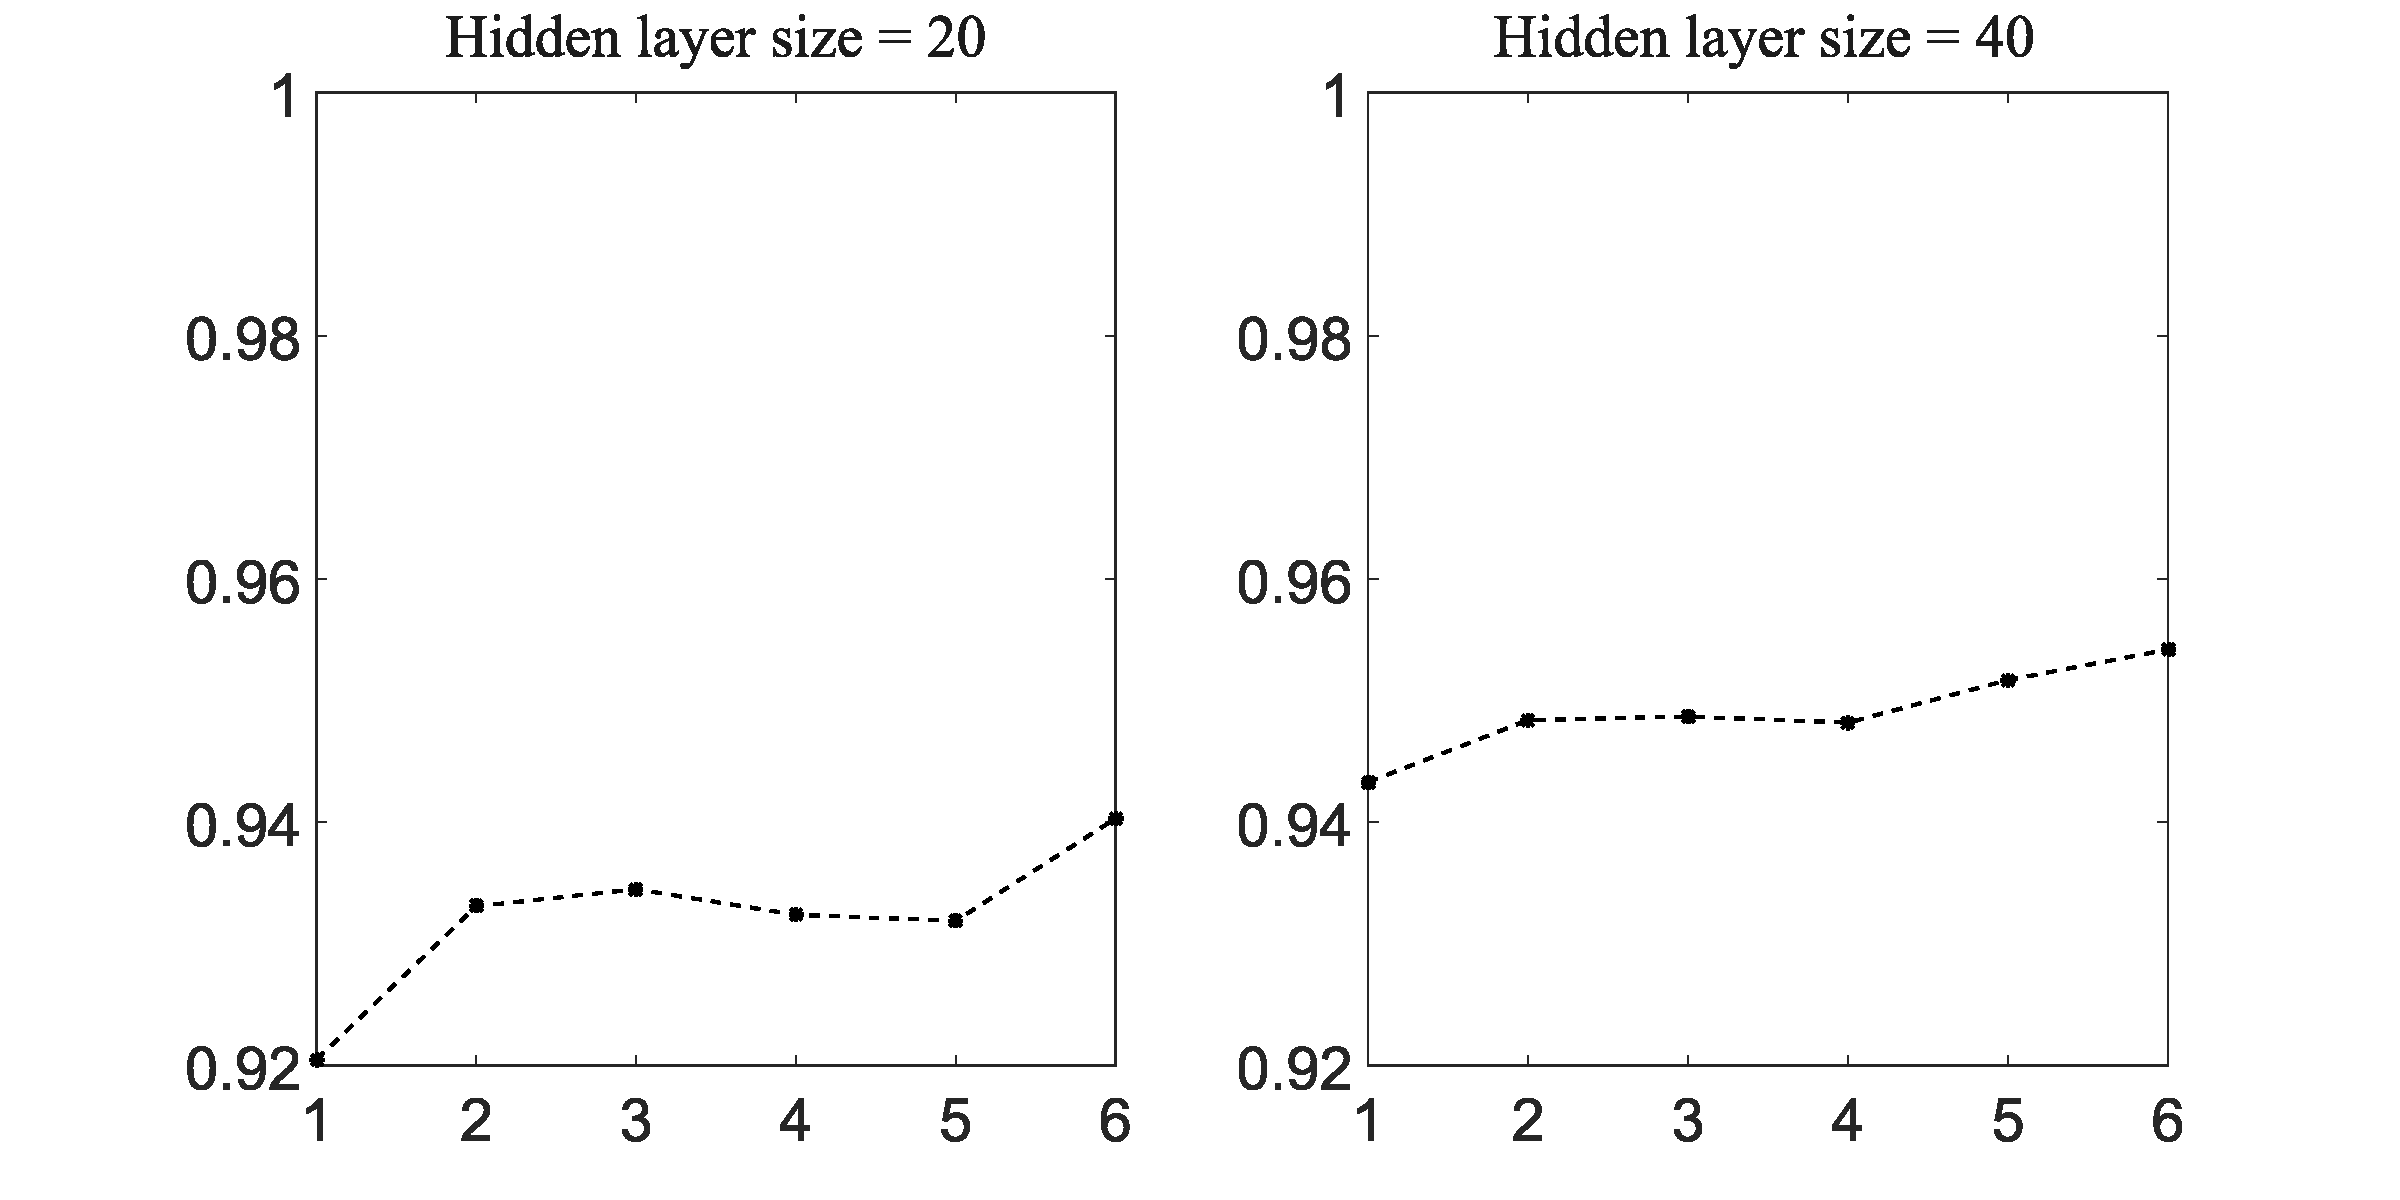
\includegraphics[width=10cm]{AccuracyTSSize_A.pdf}
\caption{Accuracy vs. Training set size}
\label{figure:AccuracyTSSizeA}
\end{figure}
\begin{figure}[tmbh]
\centering
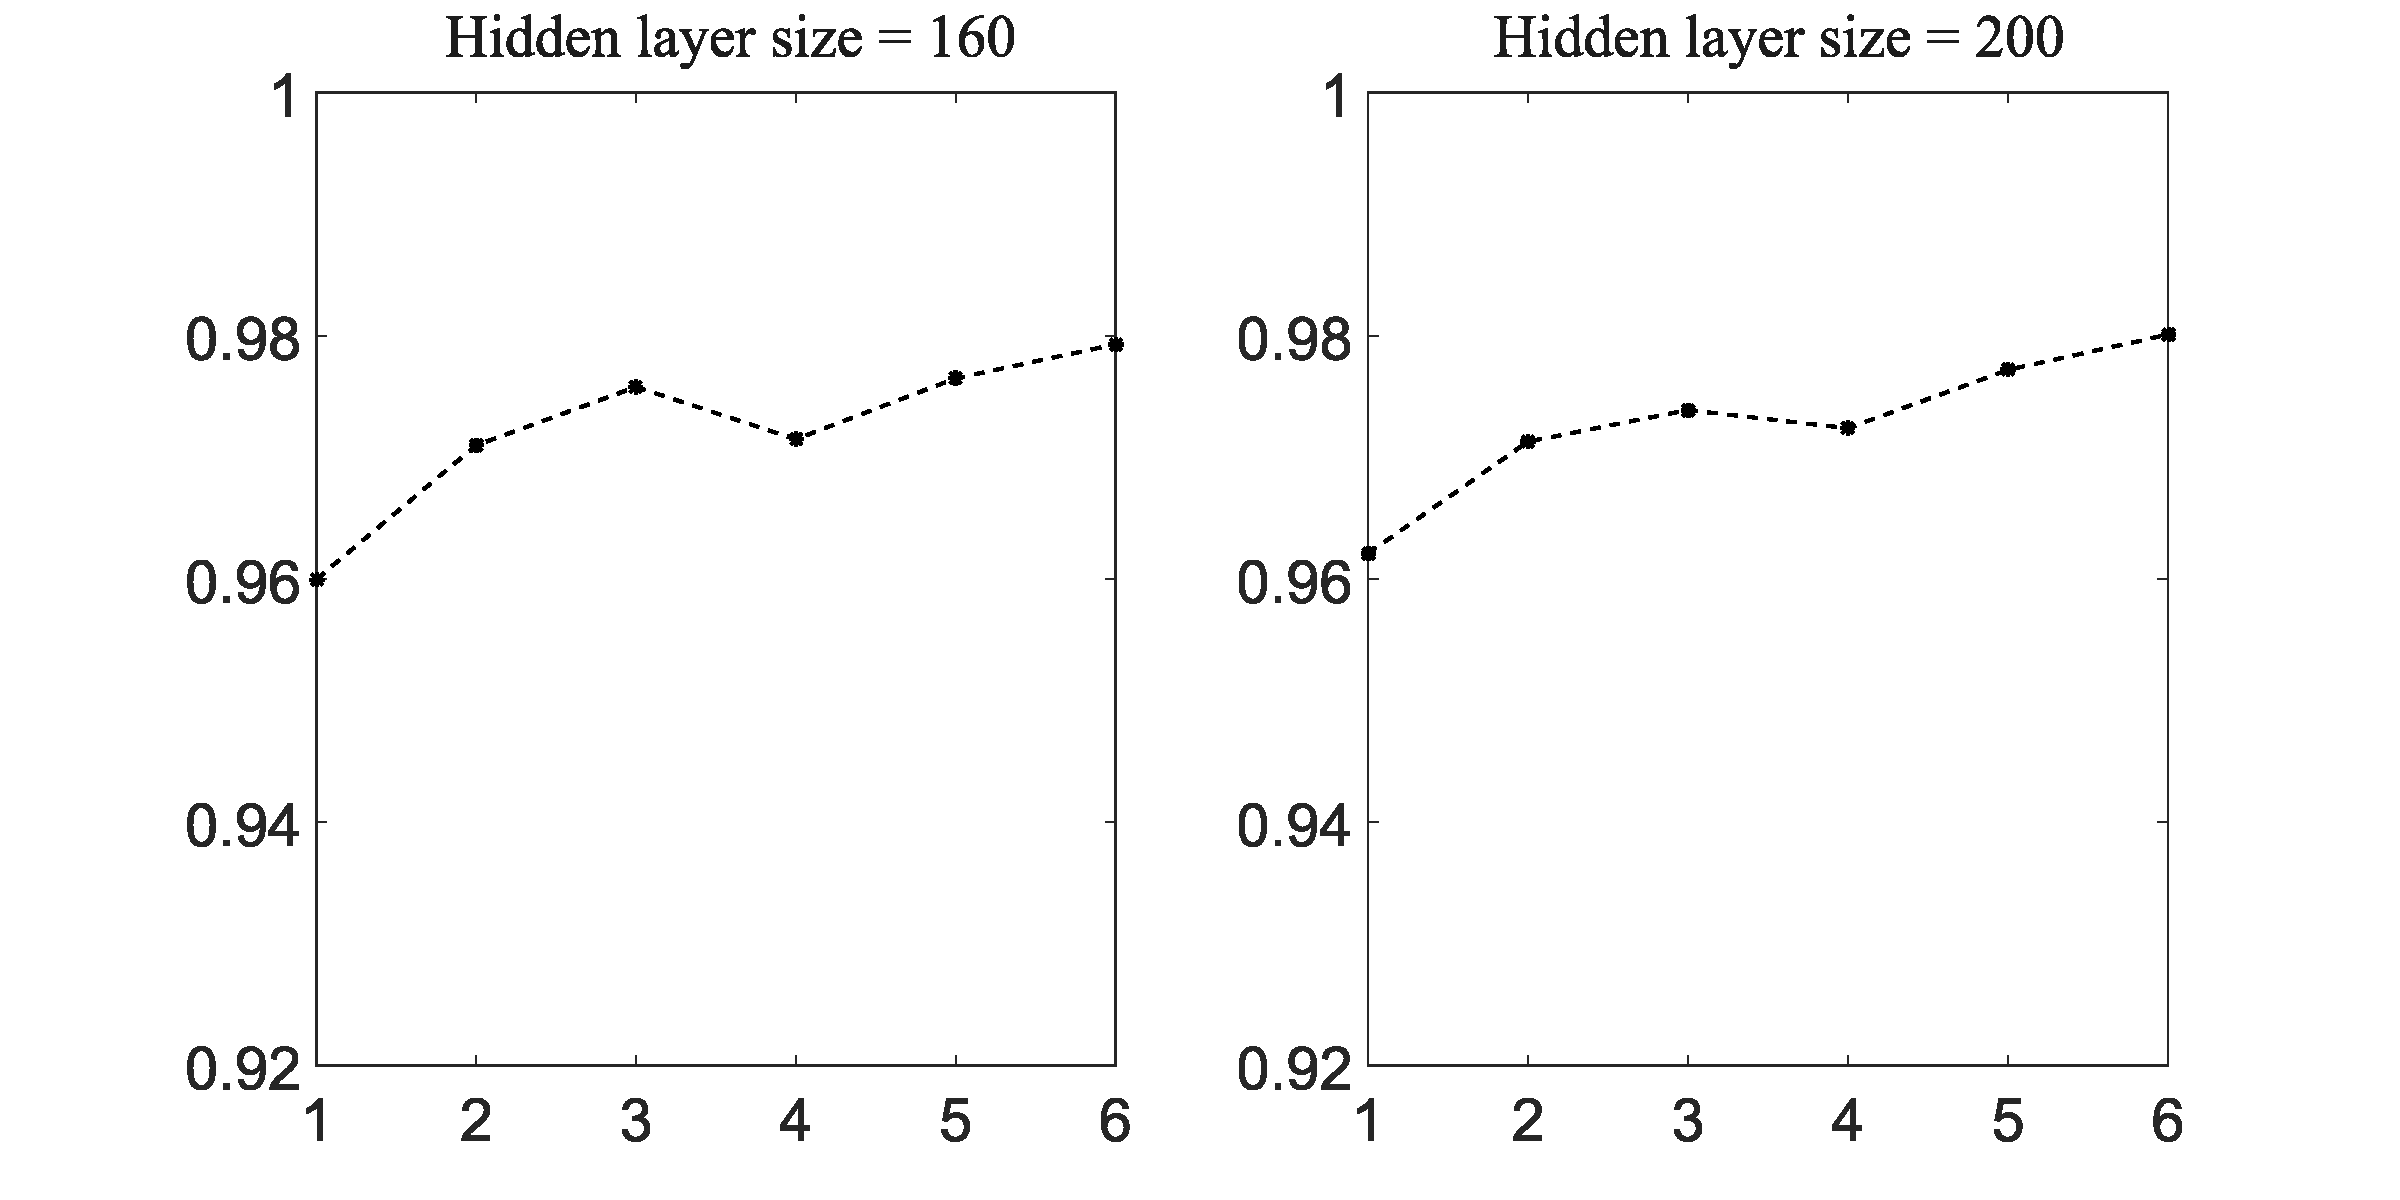
\includegraphics[width=9.8cm]{AccuracyTSSize_B.pdf}
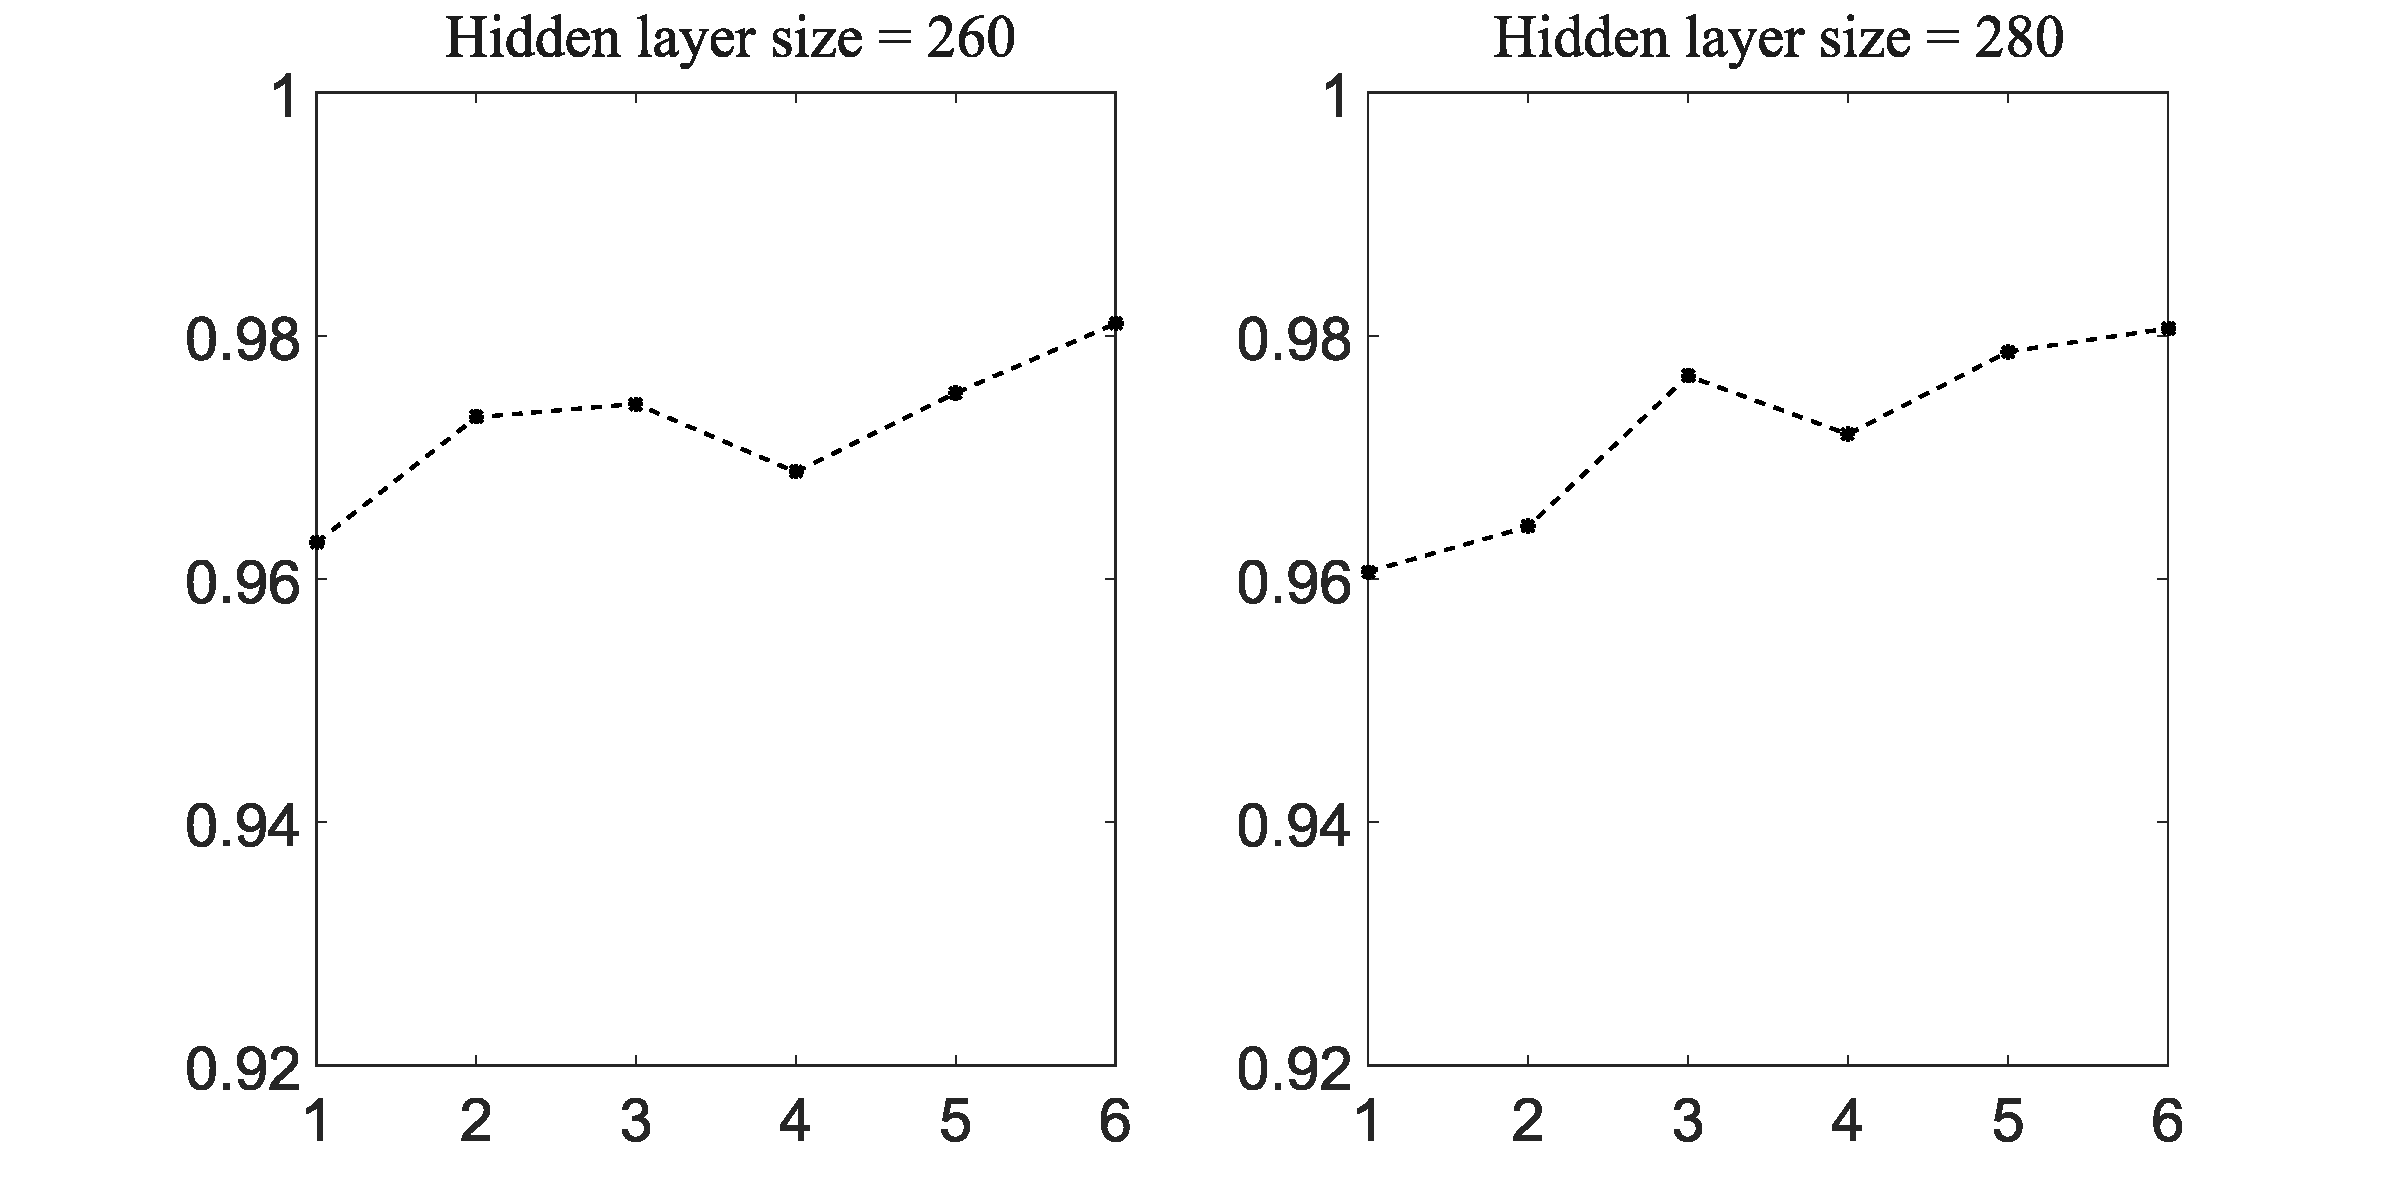
\includegraphics[width=9.8cm]{AccuracyTSSize_C.pdf}
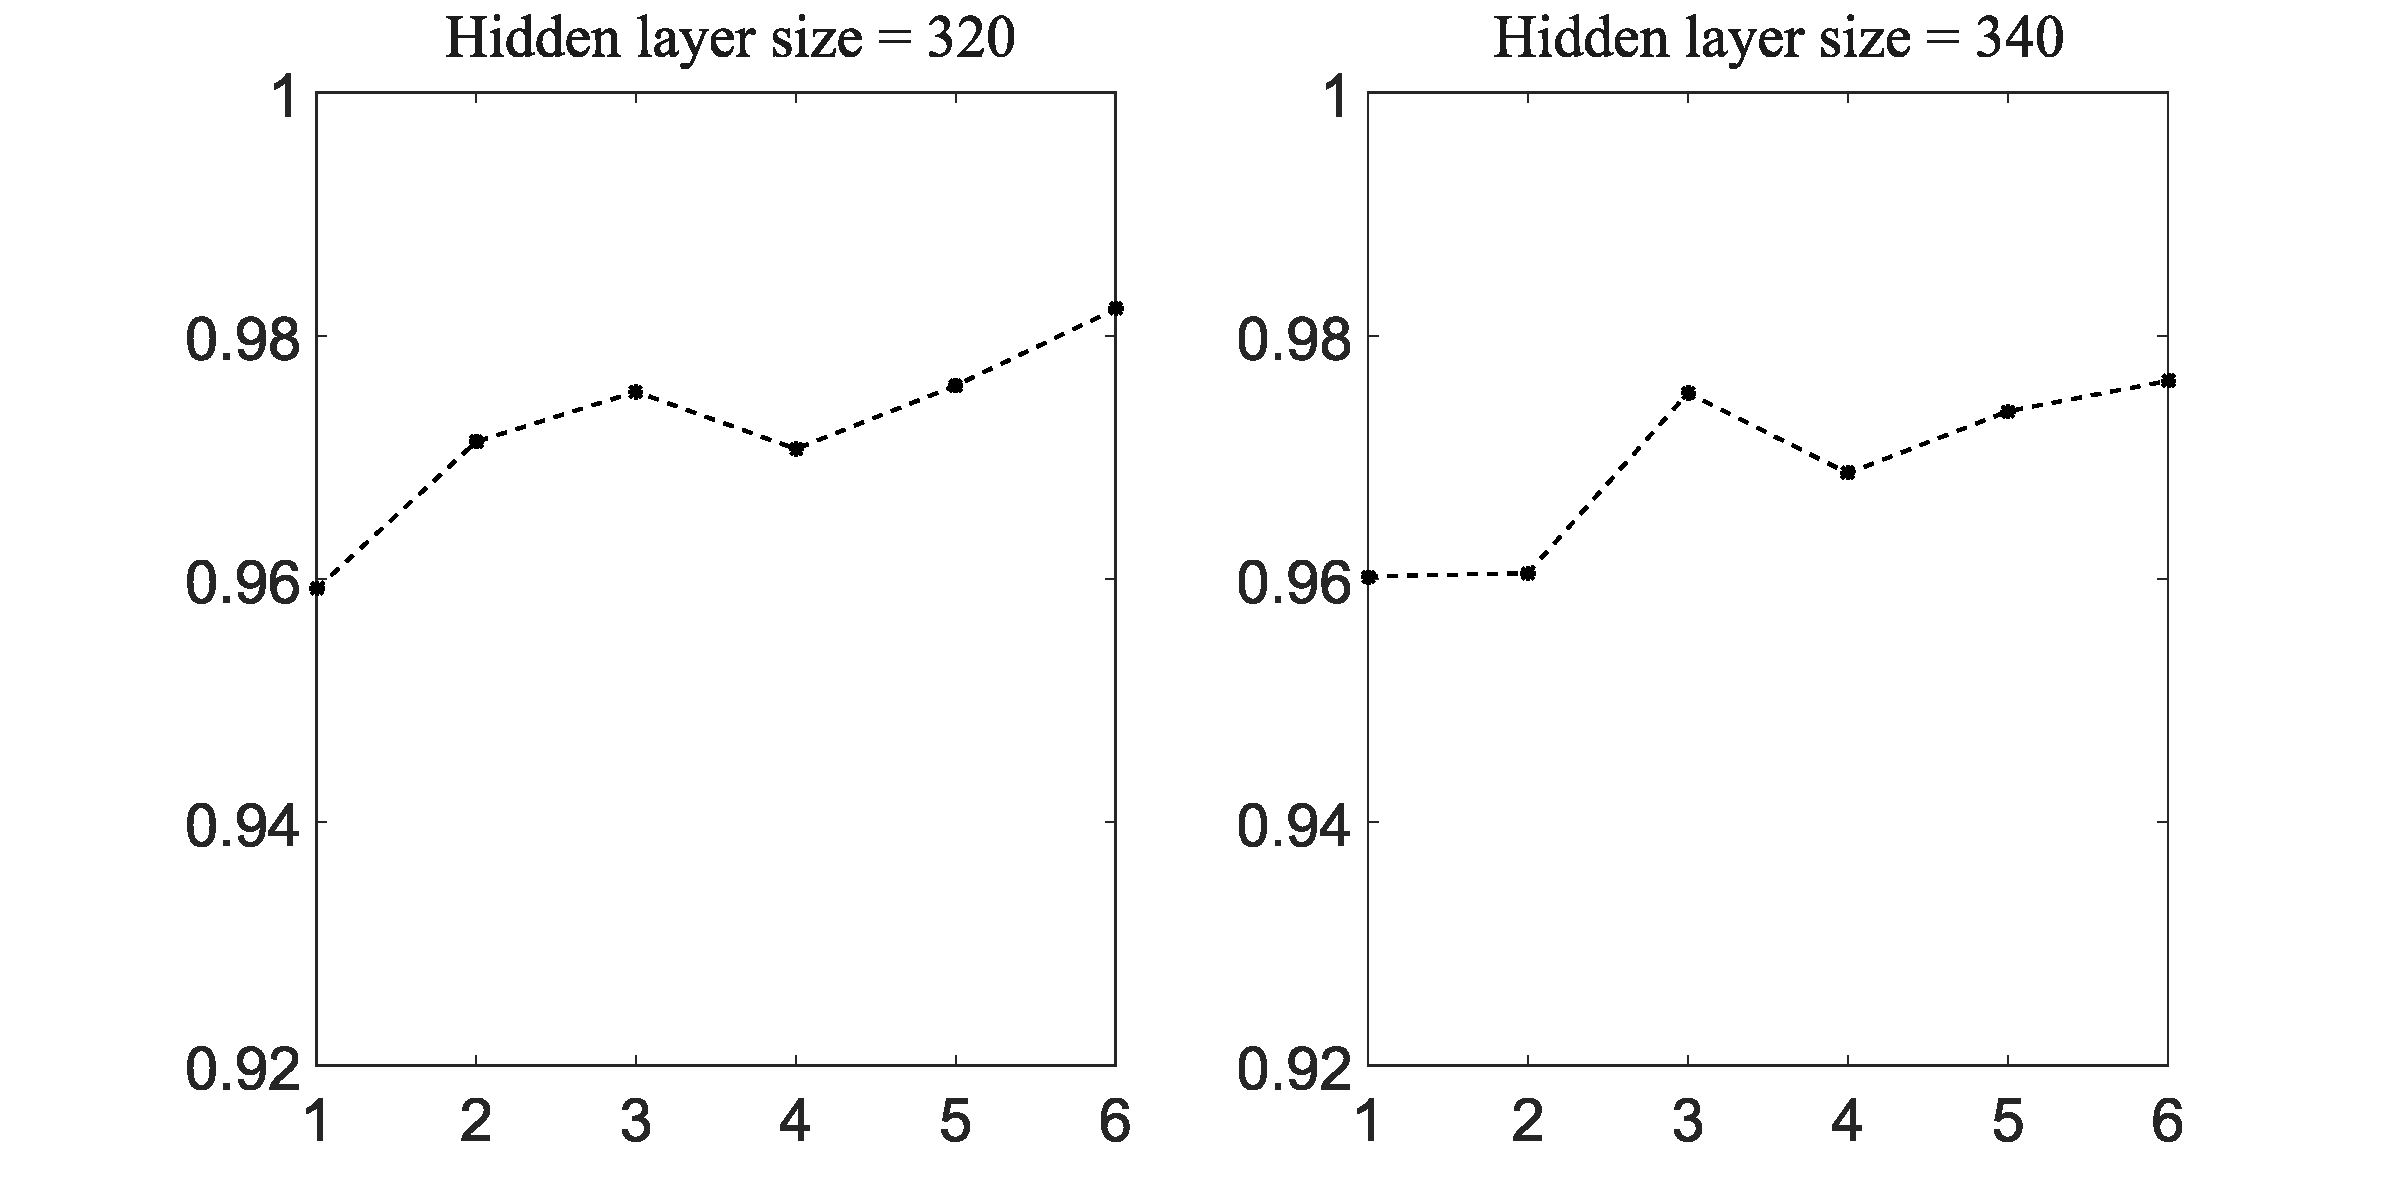
\includegraphics[width=9.8cm]{AccuracyTSSize_D.pdf}
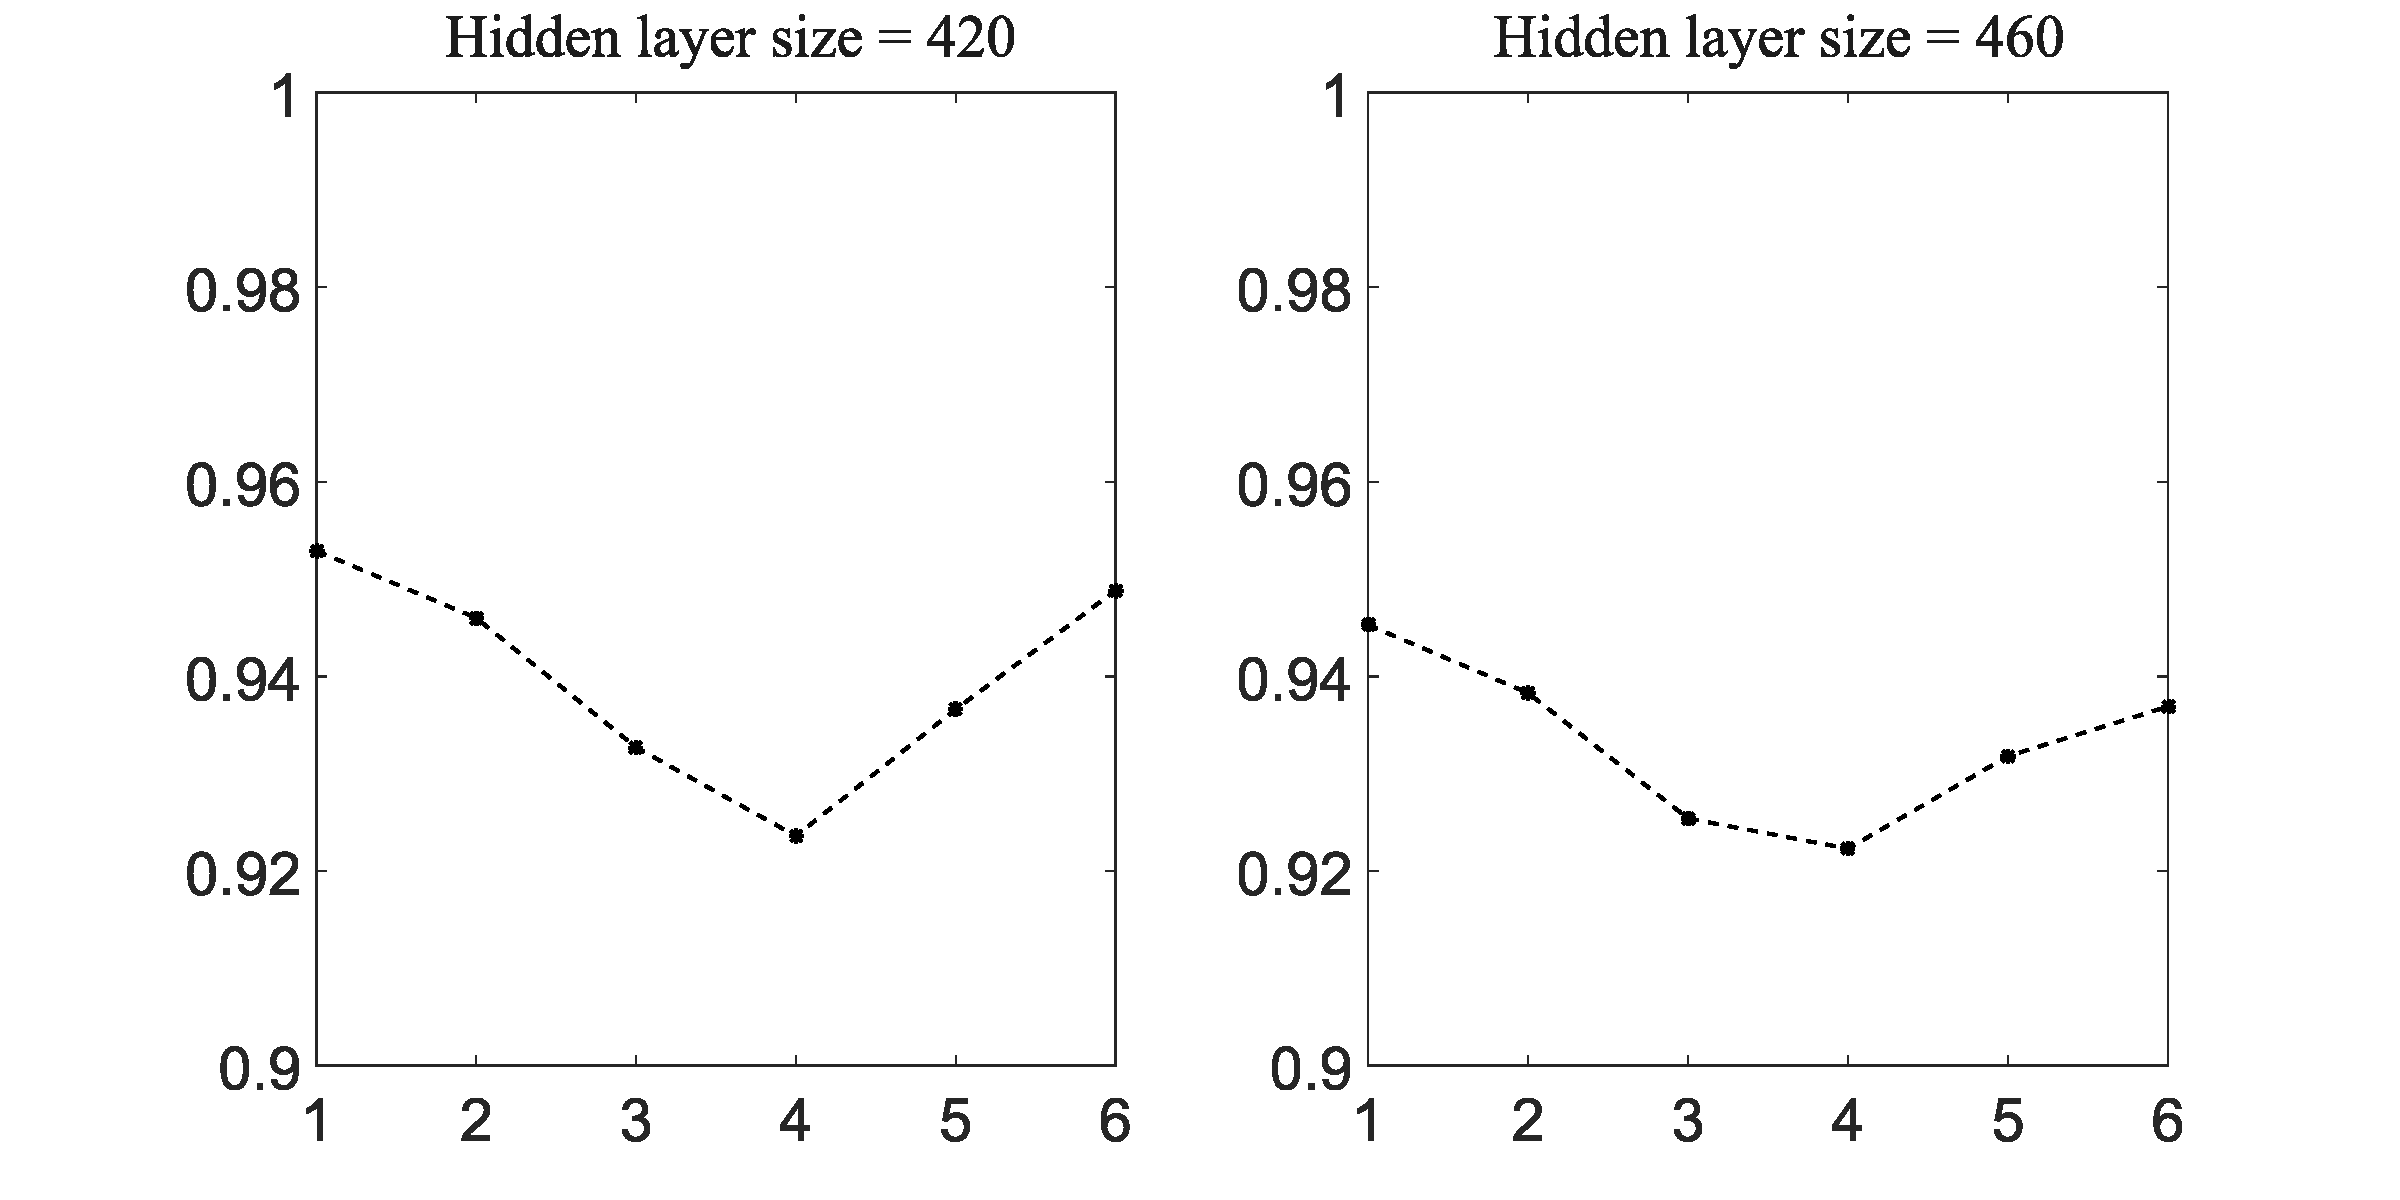
\includegraphics[width=9.8cm]{fig2ilu_b.pdf}
\caption{Accuracy vs. Training set size}
\label{figure:AccuracyTSSizeB}
\end{figure}
\end{subfigures}
\begin{figure}[tmbh]
\centering
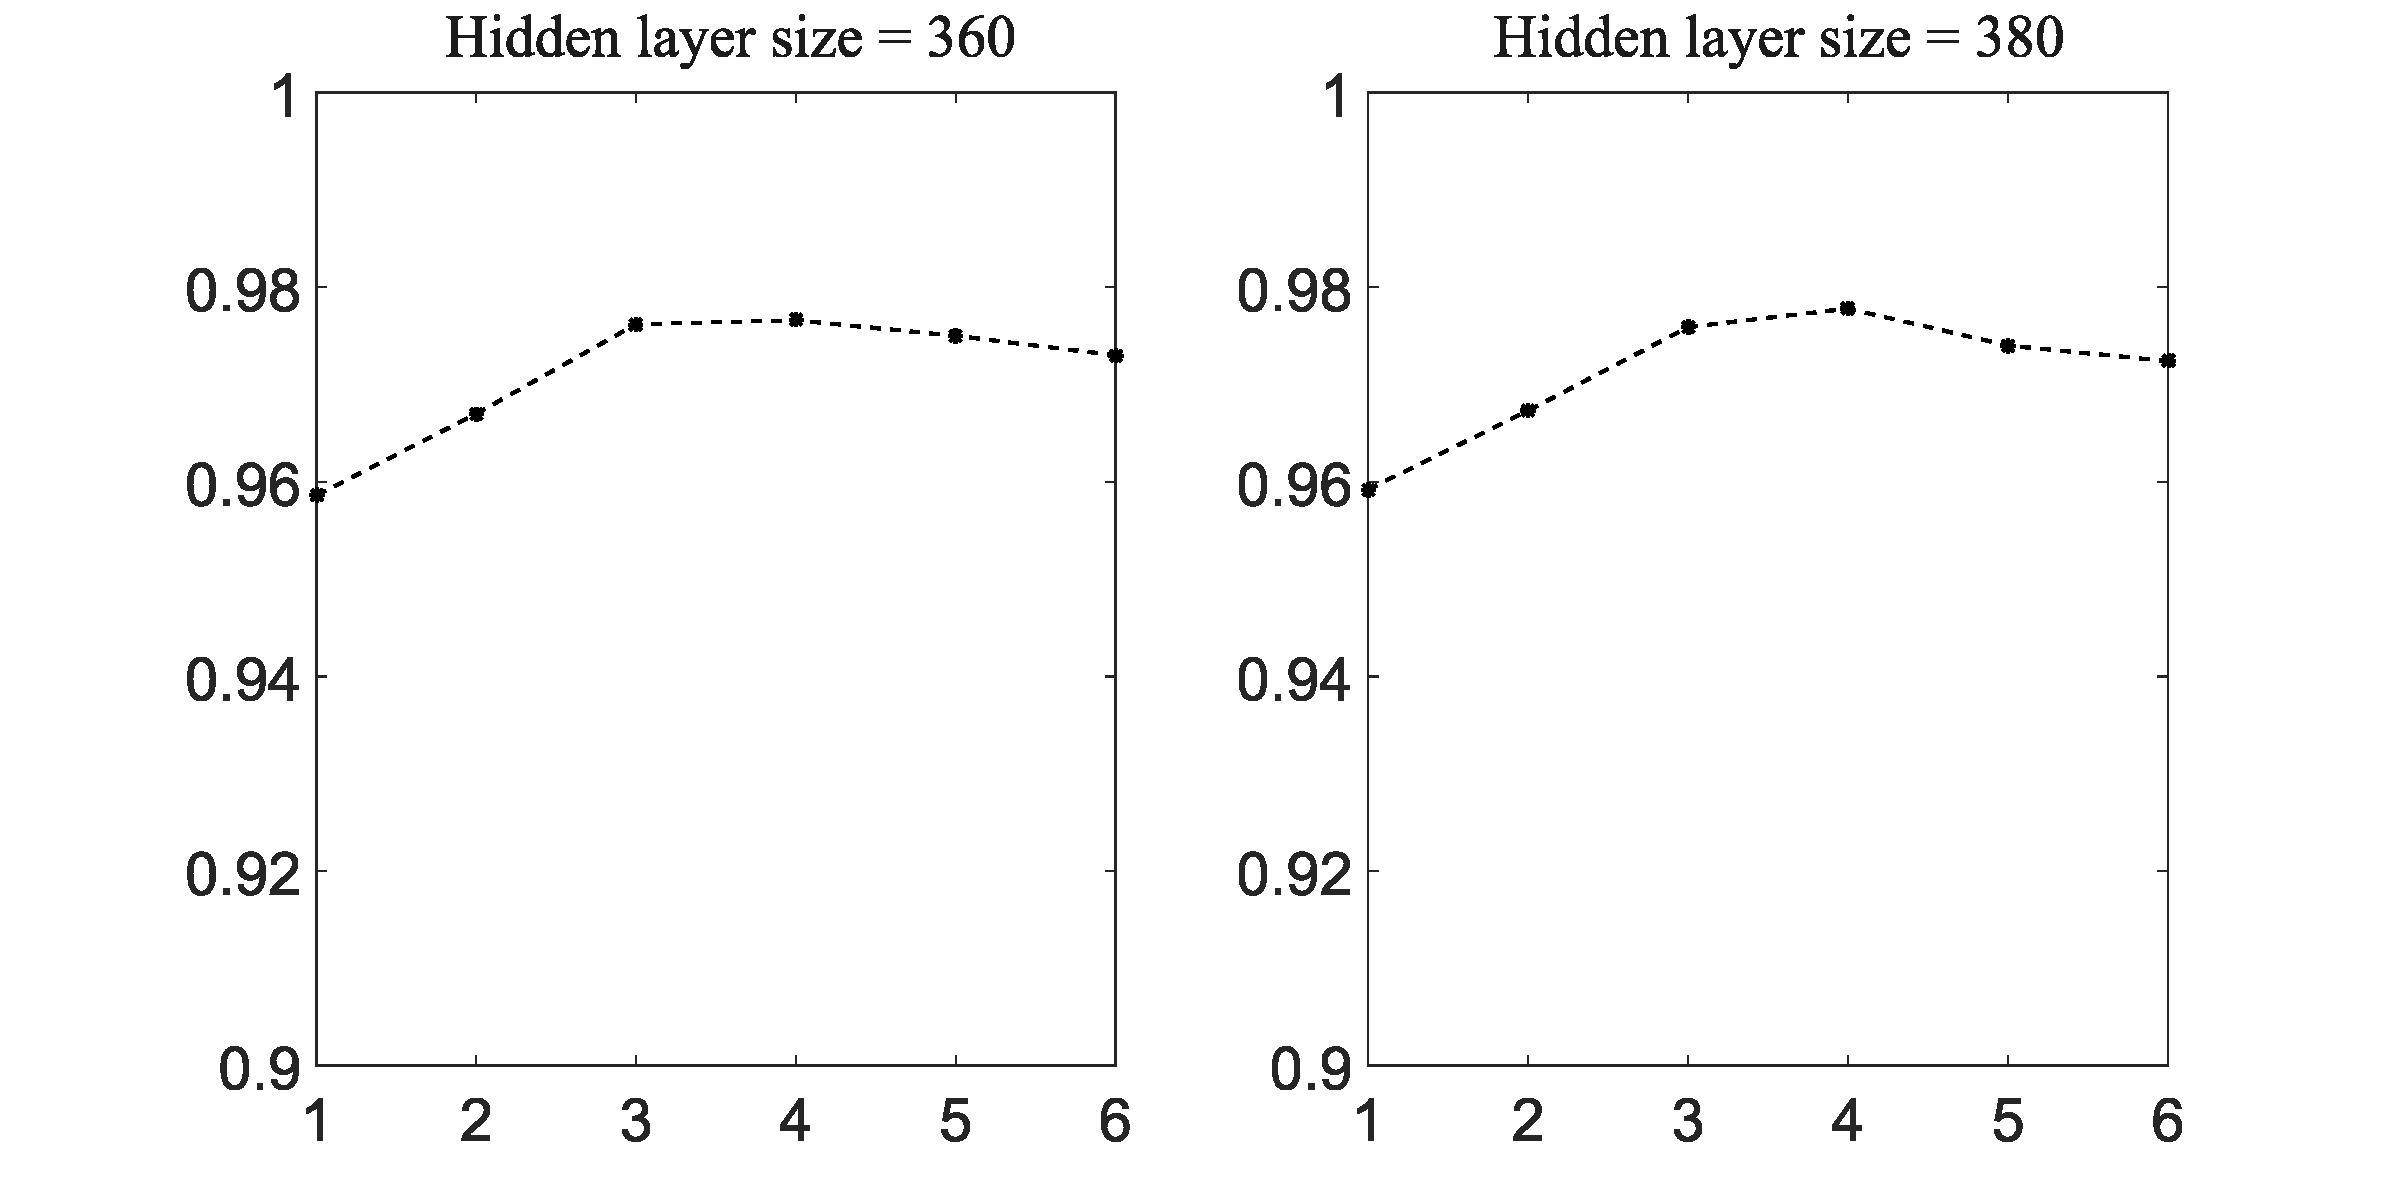
\includegraphics[width=10cm]{fig2ilu_a.pdf}
\caption{Neural networks that do not perform best on test set after full-set training}
\label{figure:fig2ilu}
\end{figure}
Table \ref{table:ClassProportionVsTrainingSet} shows the proportion of the ten classes present in six training sets, which are generated by the procedure introduced in section \ref{sec:Experiment}. It is clear that the proportions of these ten classes are relatively even by the random sampling procedure. It can be seen from the table that each of them deviates not too much from 0.1. This suggests an unbiasness presents in these six training subsets. Regarding this situation, one normally expects that all of the trained classifiers should perform on the MNIST test set approximately as well as it did on the training subset.

On a closer look, \cref{table:ClassProportionVsTrainingSet} also suggests that as the training set size increase, the unevenness between classes sizes significantly decreases, which means the dataset is more and more balanced. Thus, a classifier trained on a bigger subset should be more impartial over the ten classes, not to mention a richer source of training material it would benefit from this bigger subset. All of this is illustrated in \cref{figure:ClassProportionVarianceVsTrainingSet}, where \cref{table:ClassProportionVsTrainingSet} is summarized by its decreasing row-wise variances. In short, the general expectation that the biggest training set produces the best generalization error rate on MNIST test set is backed up by reasonably bold evidences.

Other expected results are confirmed in \cref{figure:AccuracyHLSizeA,figure:AccuracyHLSizeB}. Small sized hidden layers are too simple to fully capture the underlying patterns in both training set and test set. Neural networks with too much parameters, on the other hand, fit even noise in the data, which is harmful to their generalization. Neural networks with intermediate hidden layer size strike the balance of these two extremes. The best neural network have 180 hidden neurons trained on 60.000 images. \cref{figure:MatrixConfusion} is the confusion matrix of this case and \cref{figure:SomeConfusion} shows its most common confusions.

Although the fact that 60.000 images yield this best performance may imply more training data gives better generalization, counter-examples of this assumption present more frequently in other cases. In fact, \cref{figure:AccuracyTSSizeA,figure:AccuracyTSSizeB} shows the prediction that adding more data is not always better has successfully applied to data from the MNIST dataset. Specifically in \cref{figure:fig2ilu}, for neural networks with hidden layer sizes of 360 and 380, the full training set of 60,000 training example does not yield better result comparing to smaller training subsets. This strange effect while adding more data is clearly illustrated by the universal concave shape presented throughout all of the 10 line graphs in \cref{figure:AccuracyTSSizeA,figure:AccuracyTSSizeB} around the third, forth, and fifth training subsets. 

While this may seem counter-intuitive, related analyzed explanations on this phenomenon have been proposed\cite{FastKNNClusterBasedTrees, MNISTHandWritten}. Accordingly, the third, forth and fifth training subsets might disagree with some assumptions that most of the fully-connected neural networks have made, and since the 24 neural networks are trained based on the minimization of an empirical cost function instead of using probabilistic principled methods, i.e. Maximum Likelihood Estimation or Bayesian Inference, the training procedure may be not self-sufficient\cite{FastKNNClusterBasedTrees}. 

Unlike ARCH regression models, a mathematically rigorous analysis for this experiment remains unelaborated due to the complex nature of the mapping function represented by multilayer neural networks. The authors cease to further this point since this is beyond the purpose of our investigation.
\FloatBarrier

\section{Conclusion}
\label{sec:conclusion} 
As shown in section IV, the assumption "more data yields better accuracy" is not always true, at least on MNIST dataset. In practice, it is almost always the case that the underlying distribution is unknown and thus can not be analyzed to decide the cut-off point on the training dataset. This raises problems when one tries to reach a better generalization, since it might not always be clear that in order to do so, which part of the whole training set should be included and which part to exclude.

Problems also emerge in cases when one attempt to compare the accuracy between different models after training them on the same dataset. For example, consider the case when a mathematician are choosing between two models A and B to interpret the data that he/she observed. Suppose the accuracy on test set is represented in the \cref{table:perform}:

\begin{table}[ht]
\caption{Performance on test set of two different models} % title of Table
\centering % used for centering table
\begin{tabular}{|c|c|c|c} % centered columns (4 columns)
\hline %inserts double horizontal lines
 { } & Training Set 1 & Training Set 2 \\ [0.5ex] % inserts table 
%heading
\hline % inserts single horizontal line
Model A & A1 & A2 \\ % inserting body of the table
Model B & B1 & B2 \\ [1ex] % [1ex] adds vertical space
\hline %inserts single line
\end{tabular}
\label{table:perform} % is used to refer this table in the text
\end{table}

In case Training Set 1 has a bigger size than Training Set 2, it is expected that $A1 > A2$ and $B1 > B2$, hence the decision depends on the comparison between $A1$ and $B1$. However, it has been shown that there might be unexpected case such as $A1 > A2$ but $B1 < B2$. If this happened, it would require further analysis on whether he/she should decide by comparing $A1$ with $B1$ or $A1$ with $B2$.



\bibliographystyle{IEEEtran}
\bibliography{IEEEabrv,mybib}

\appendix
\cref{figure:ATSS_A,figure:ATSS_B,figure:ATSS_C}  shows the performance on MNIST test set of 24 neural networks after training them on 6 training subsets.

\begin{subfigures}
\begin{figure}[tmbh]
\centering
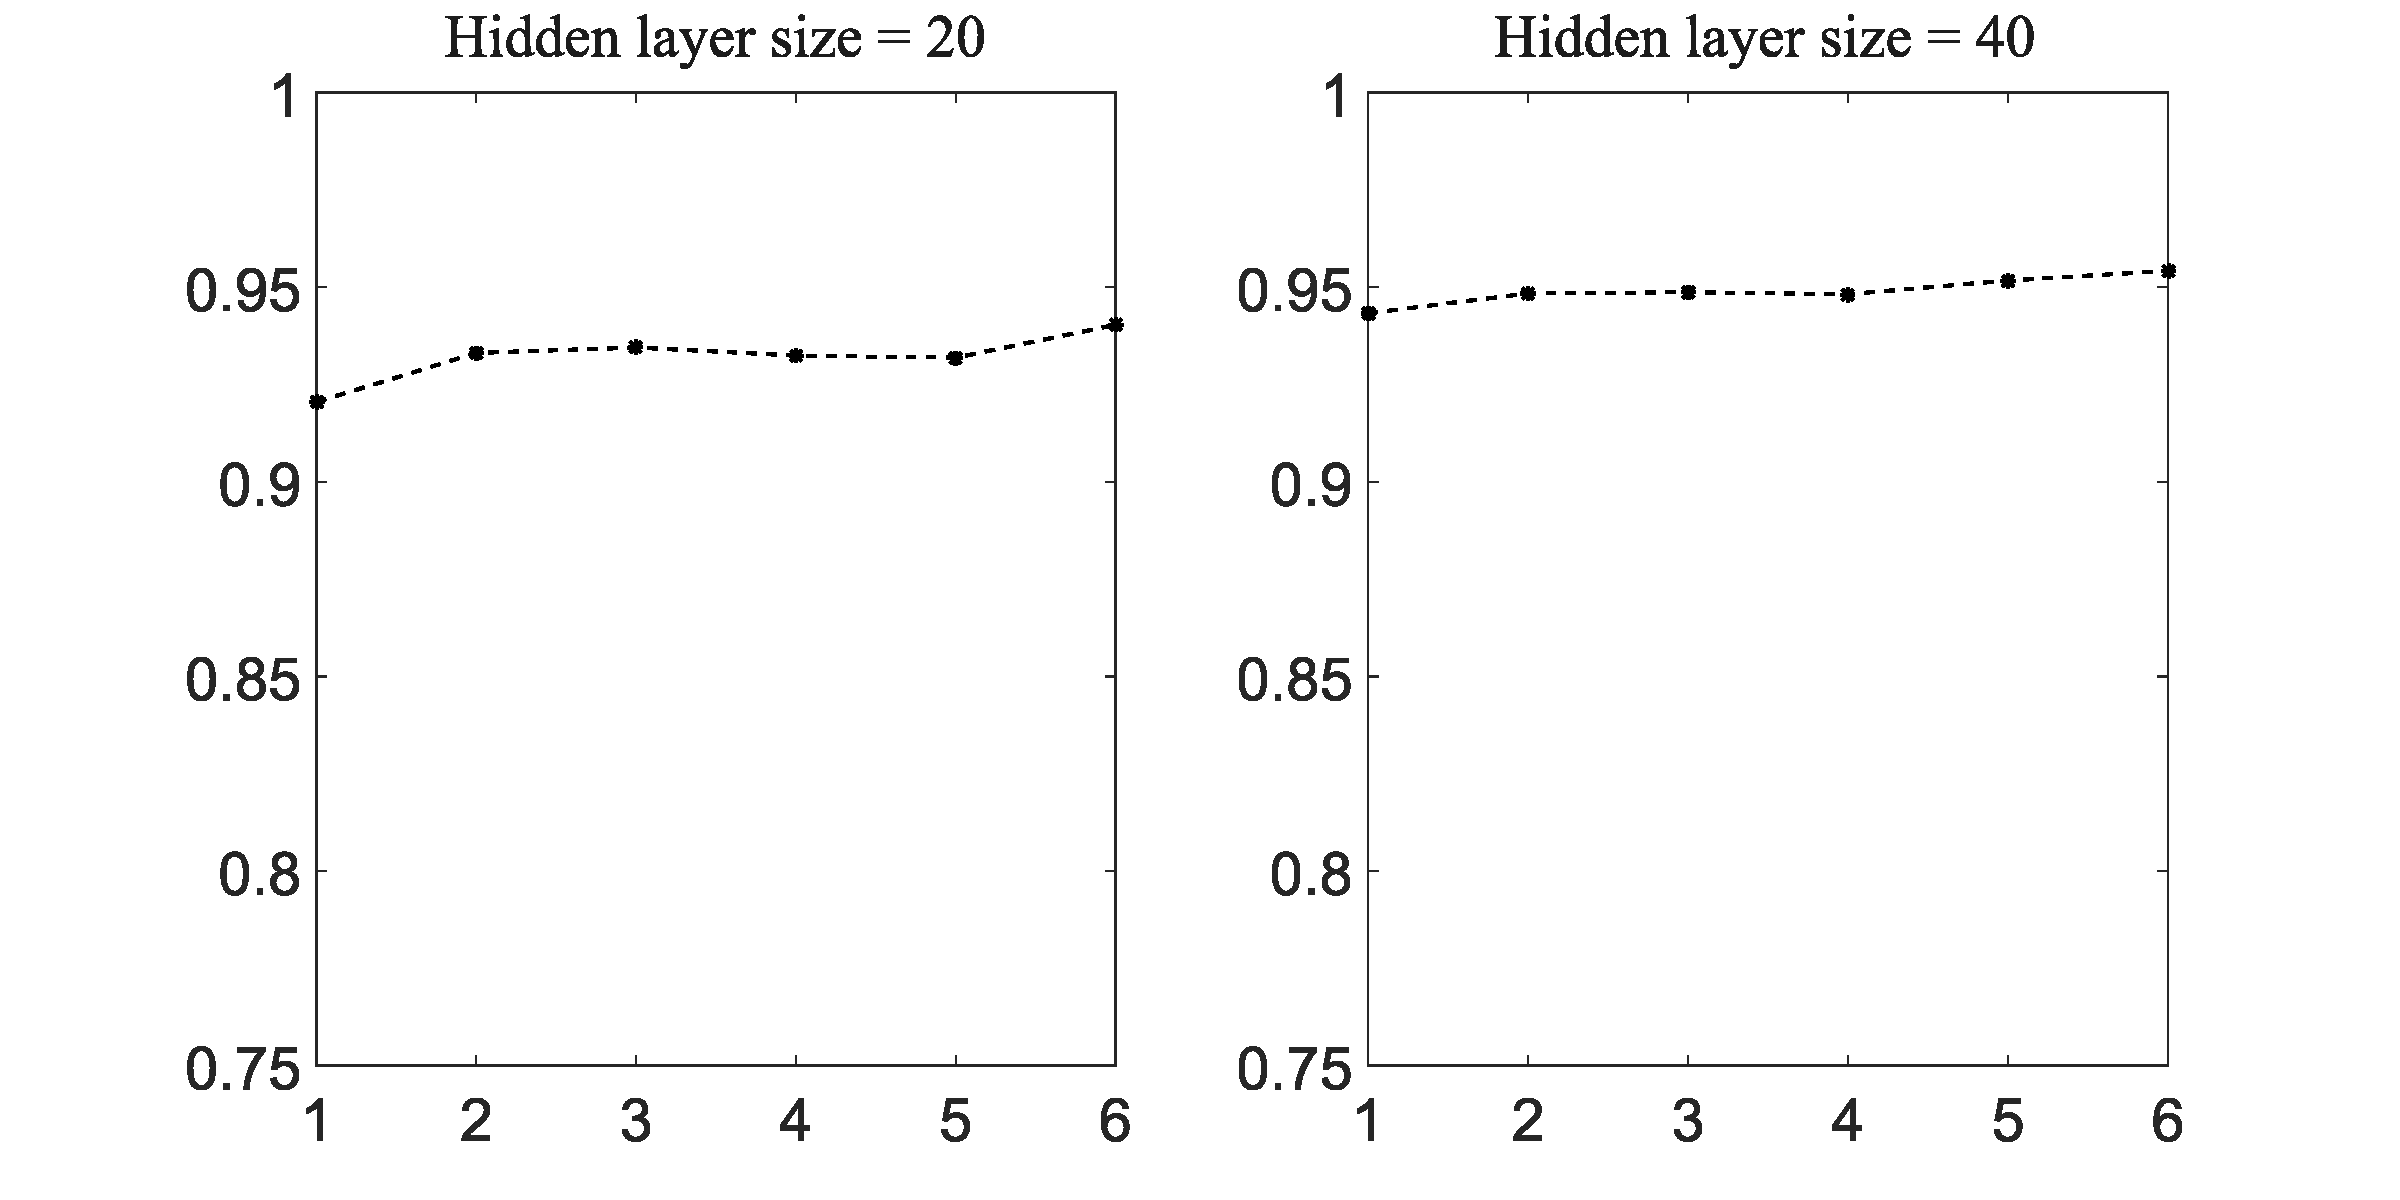
\includegraphics[width=10cm]{AccuracyTSSizeA.pdf}
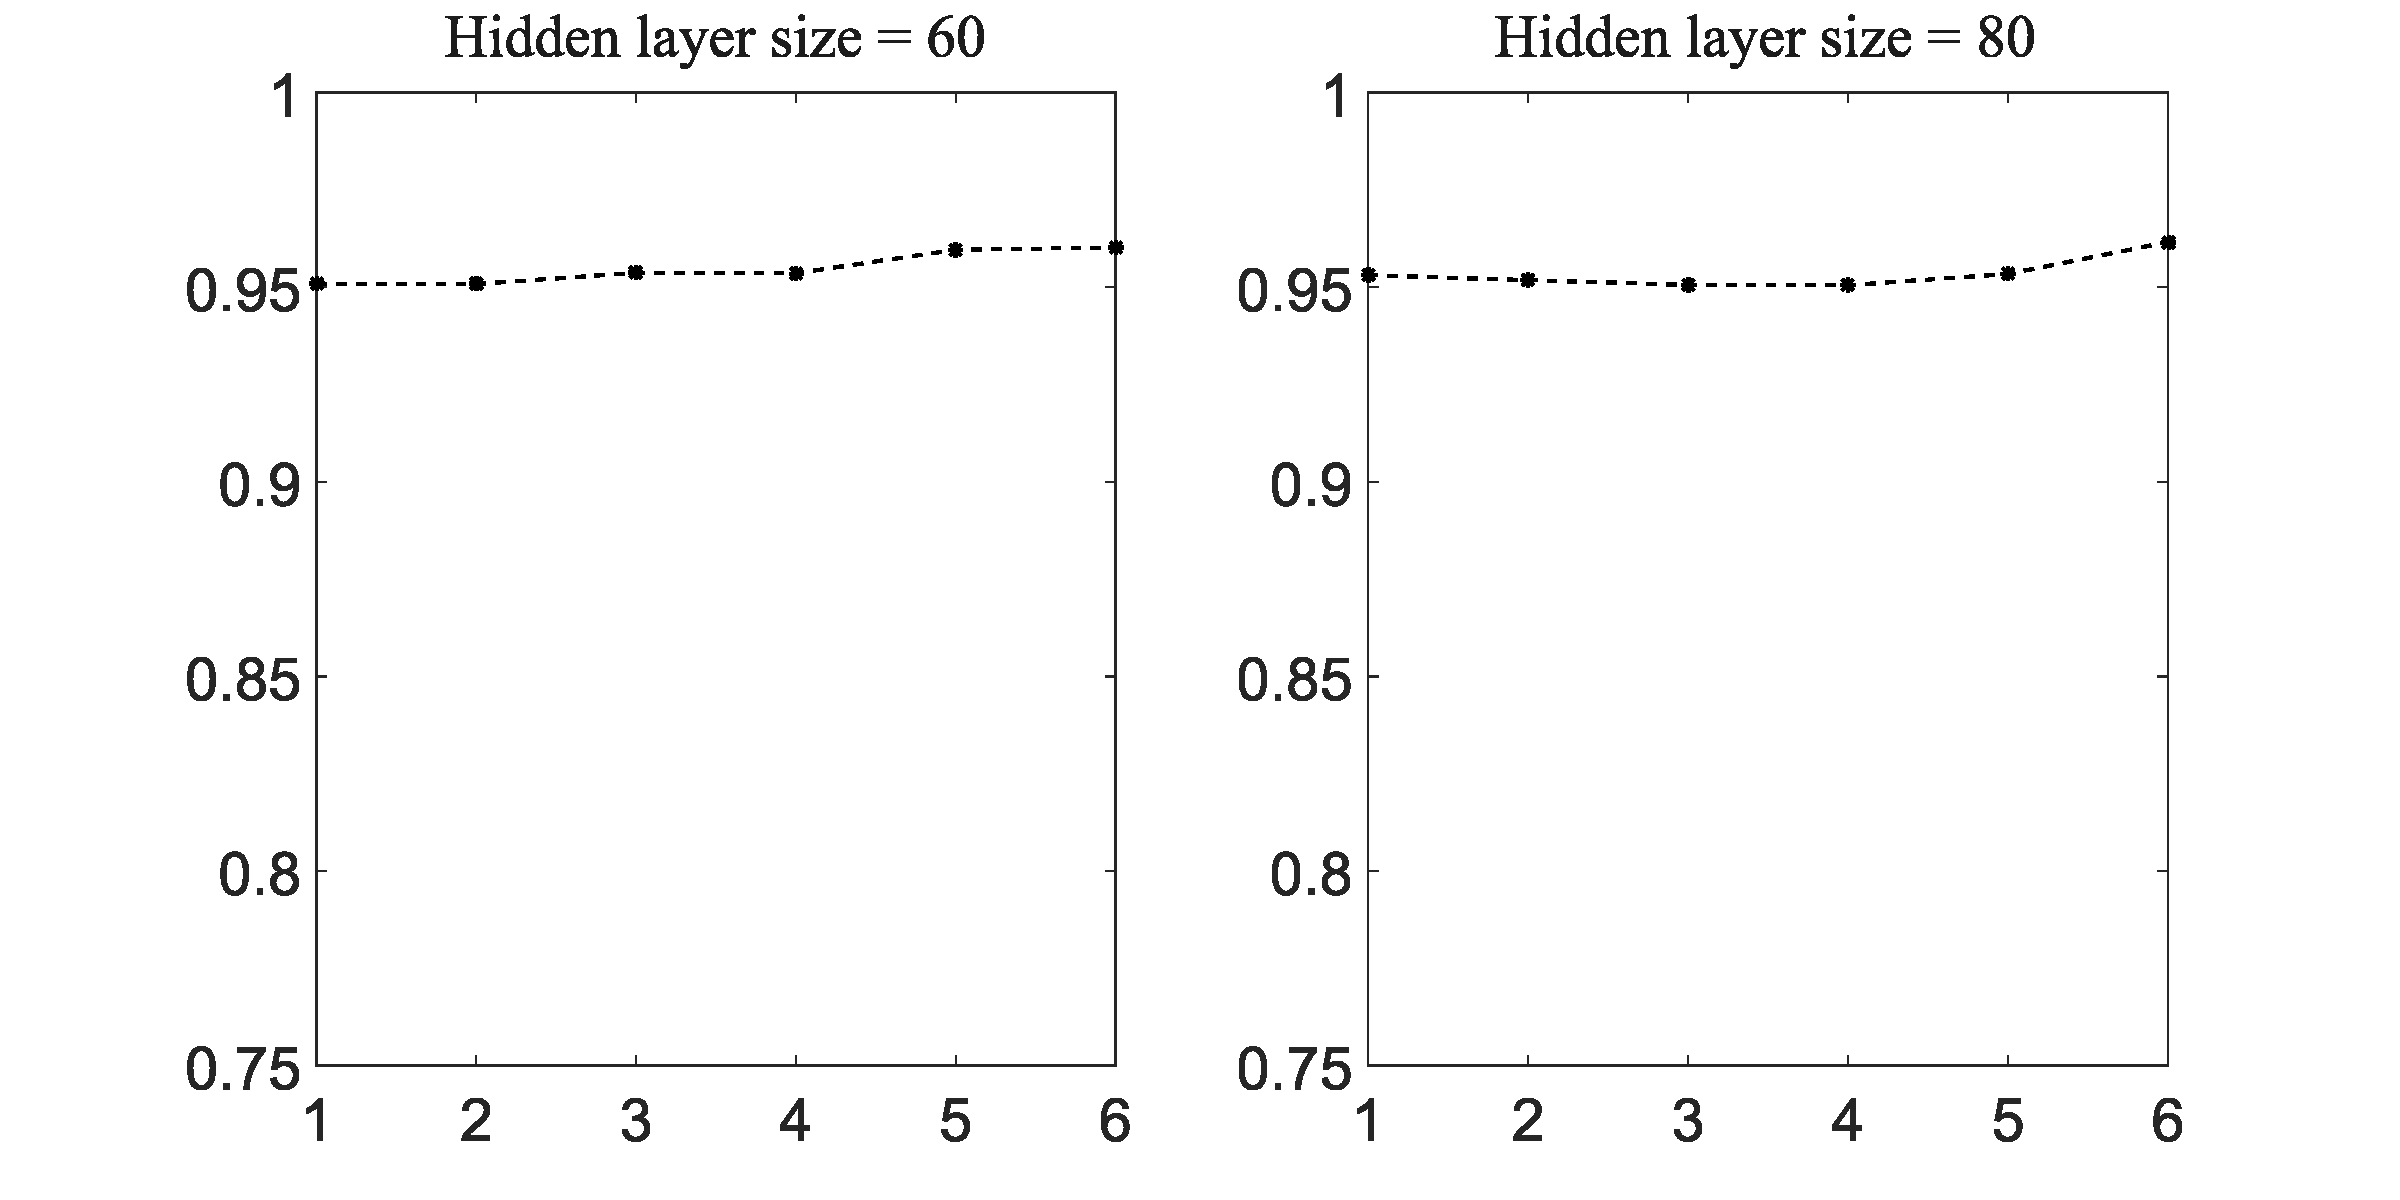
\includegraphics[width=10cm]{AccuracyTSSizeB.pdf}
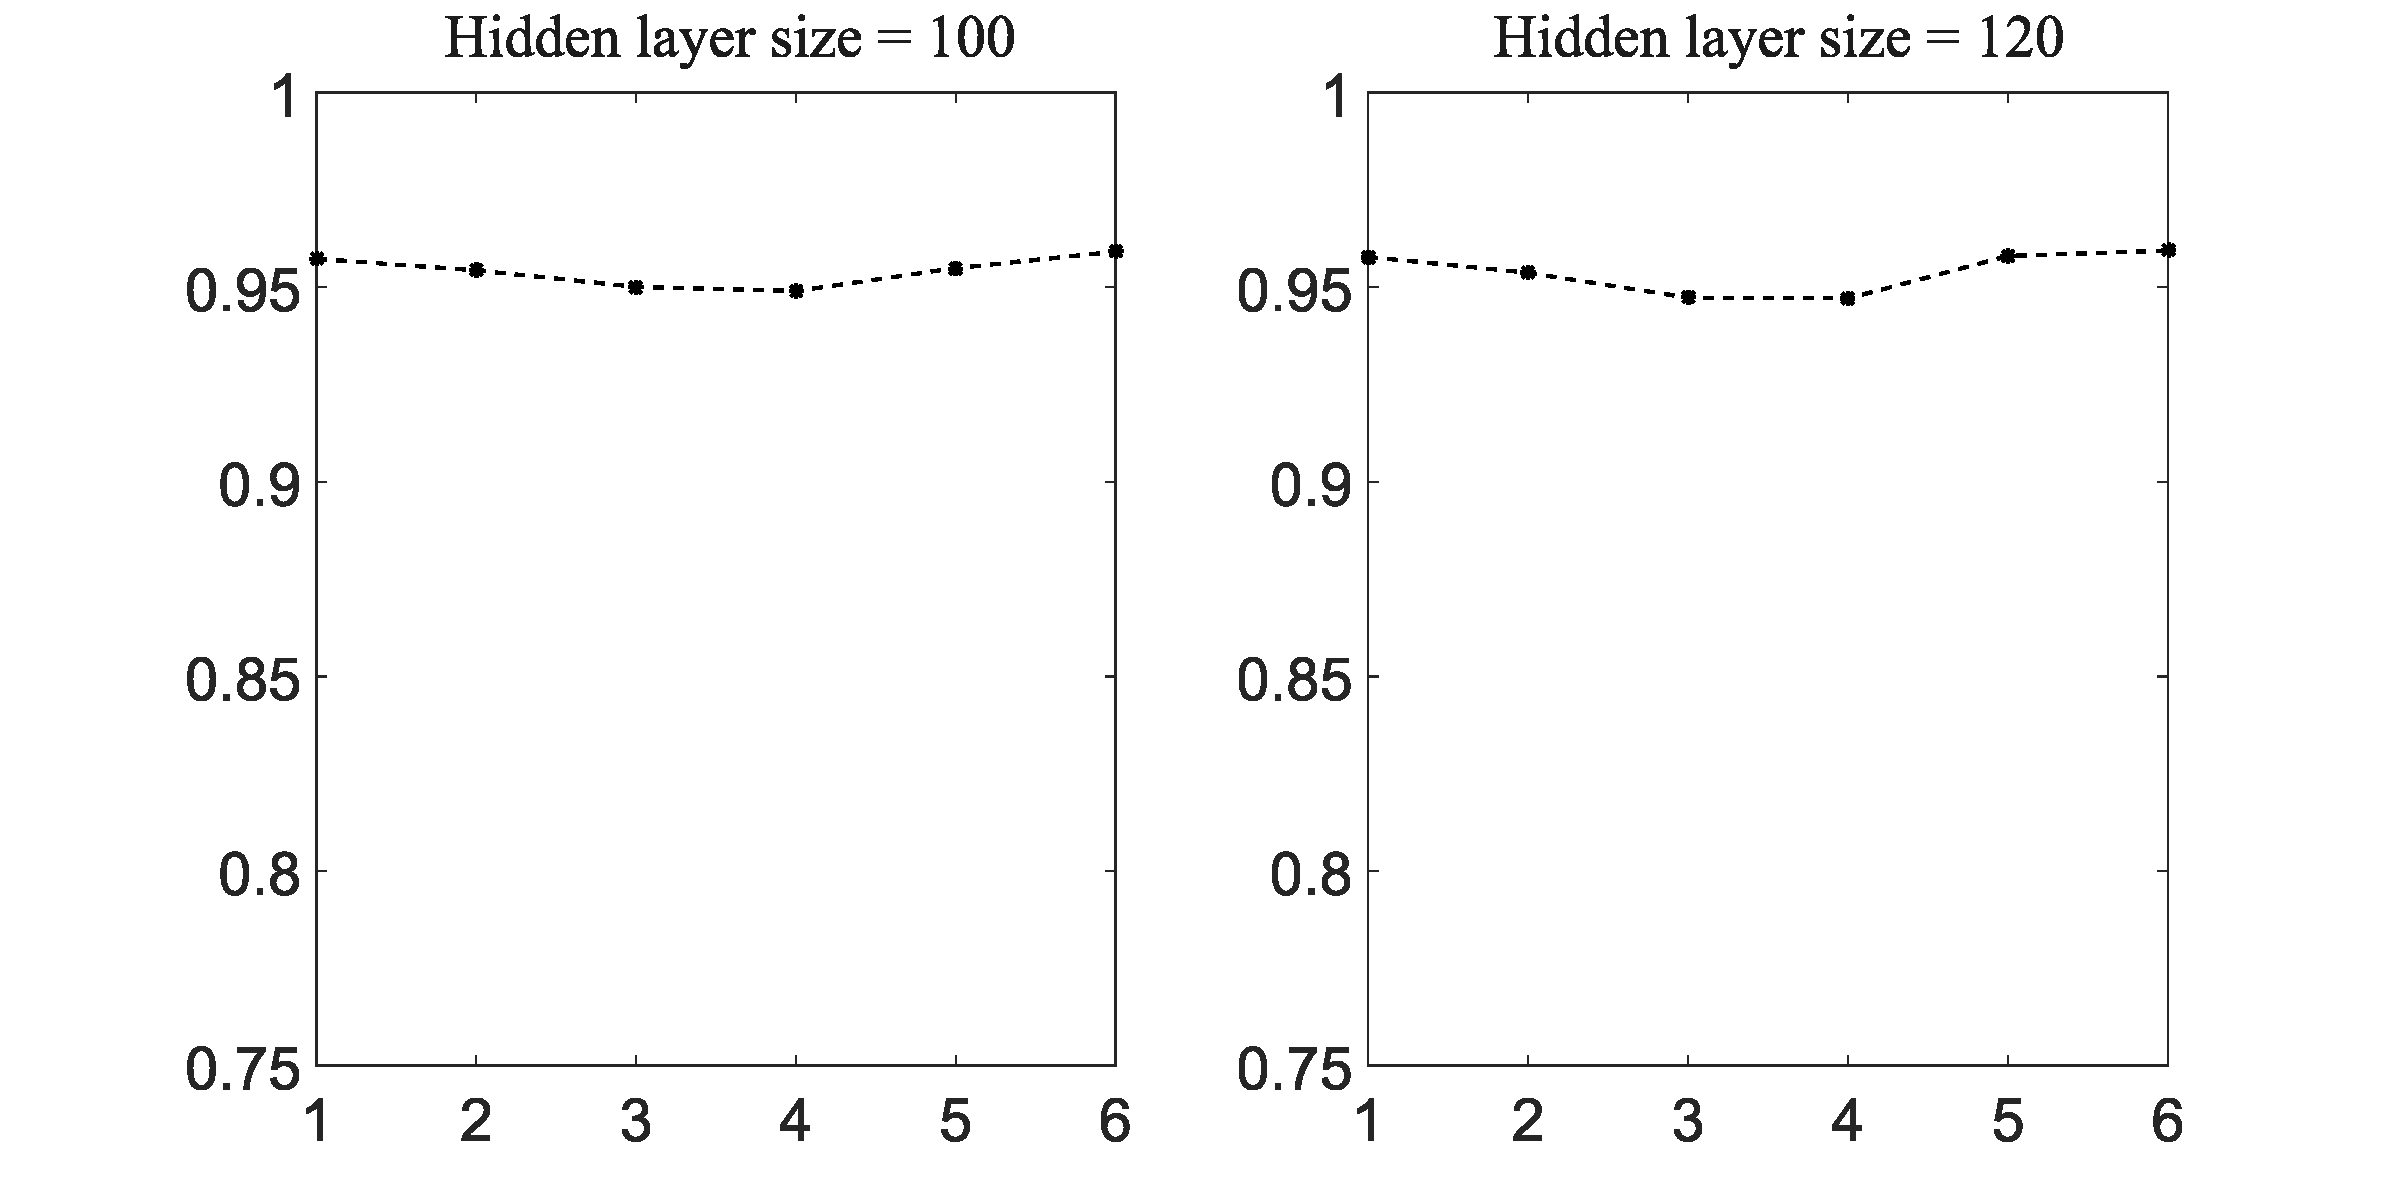
\includegraphics[width=10cm]{AccuracyTSSizeC.pdf}
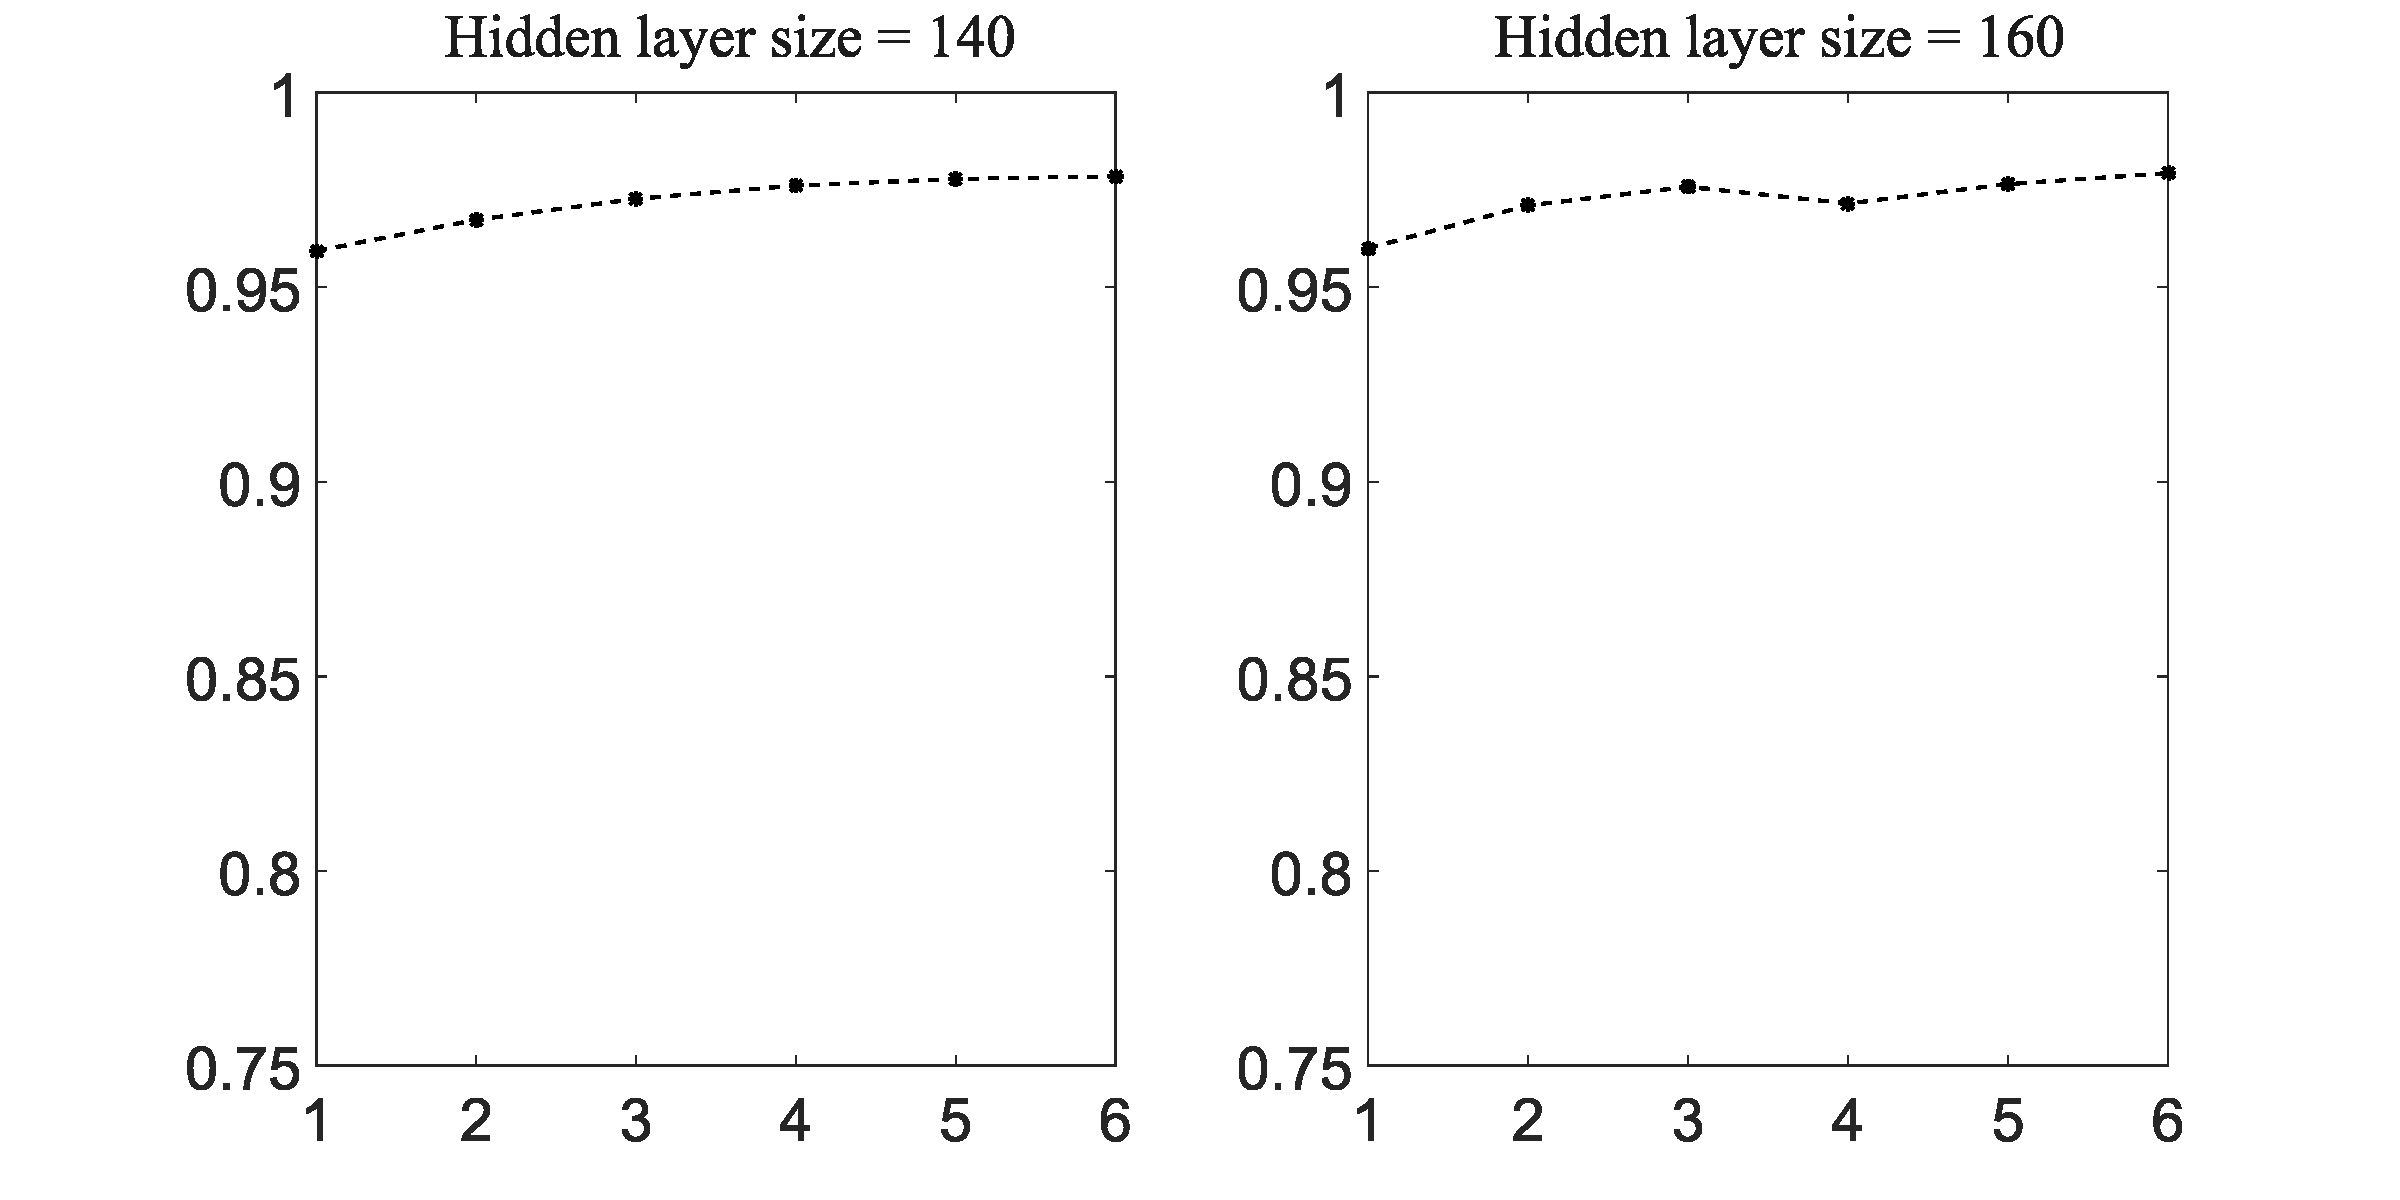
\includegraphics[width=10cm]{AccuracyTSSizeD.pdf}
\caption{Accuracy vs. Training set size}
\label{figure:ATSS_A}
\end{figure}

\begin{figure}[tmbh]
\centering
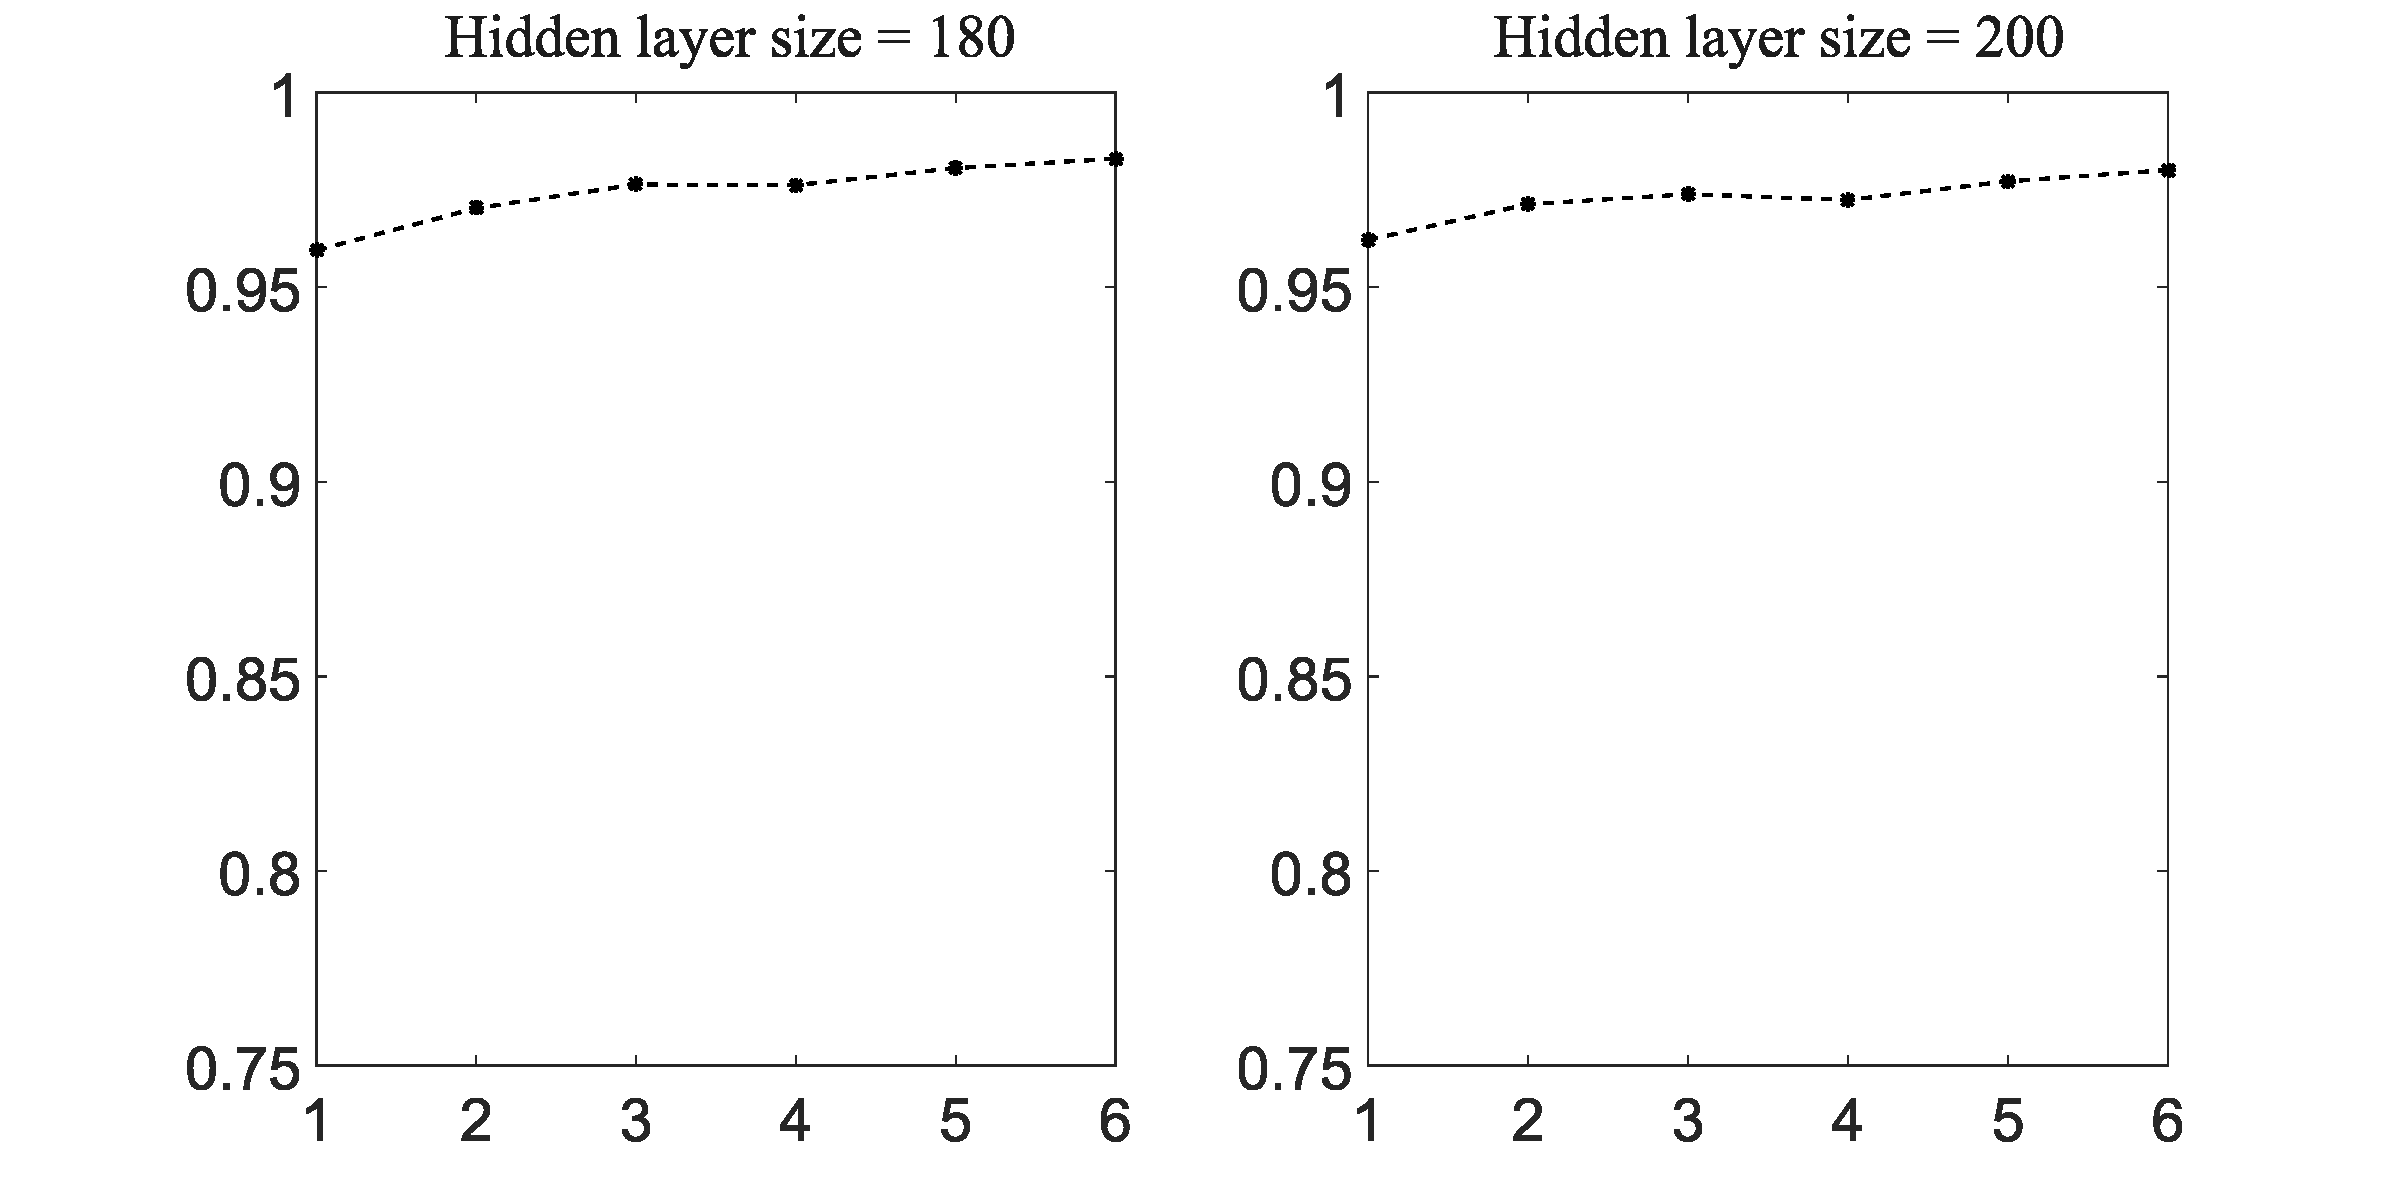
\includegraphics[width=10cm]{AccuracyTSSizeE.pdf}
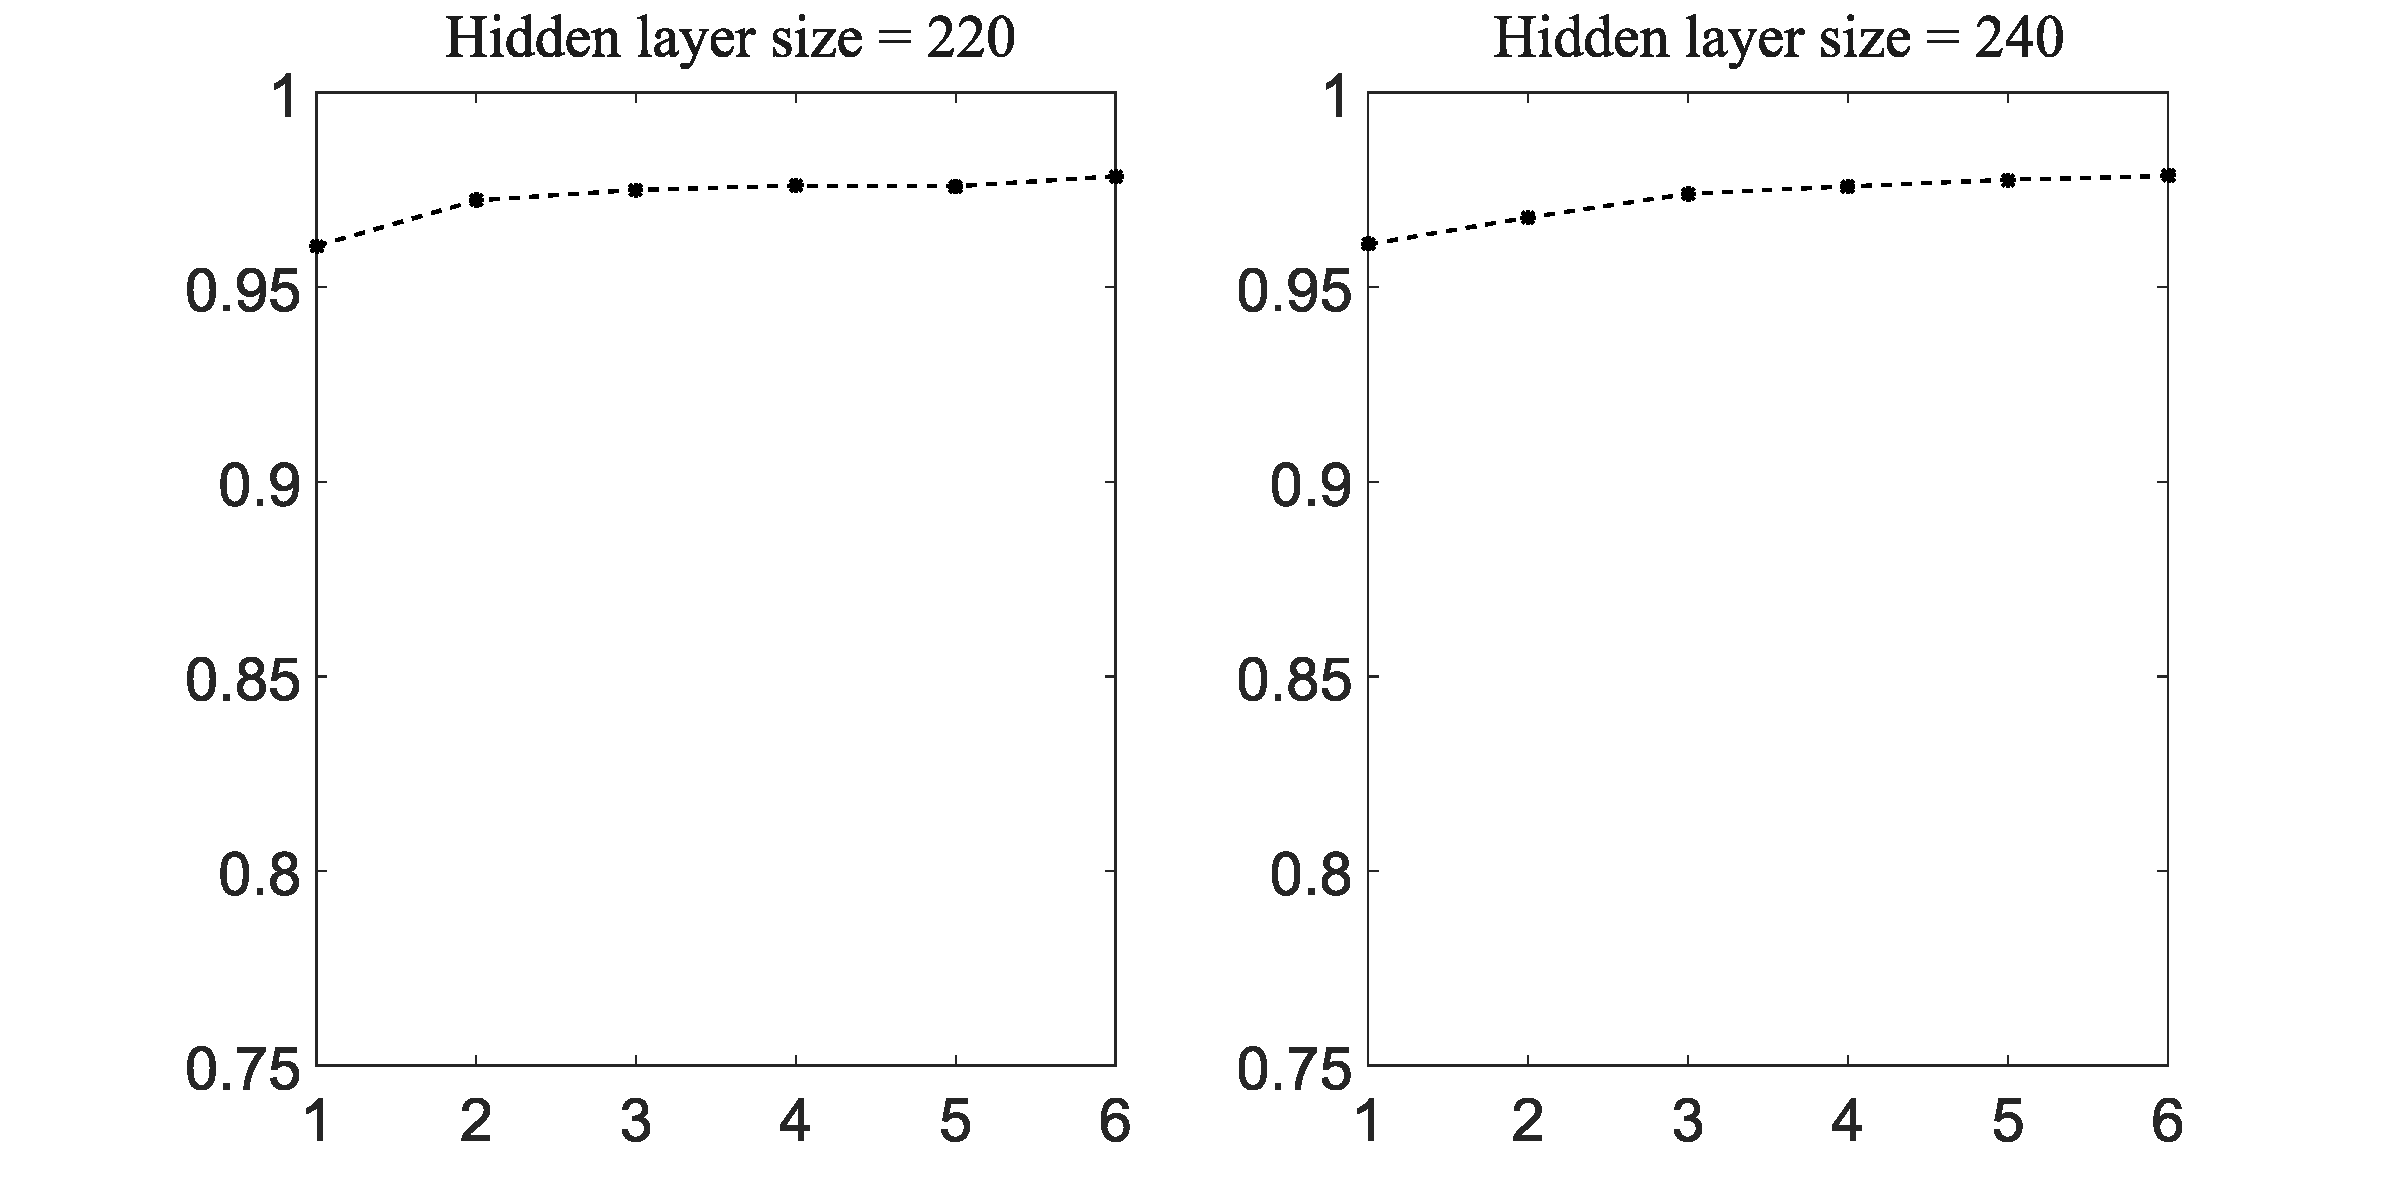
\includegraphics[width=10cm]{AccuracyTSSizeF.pdf}
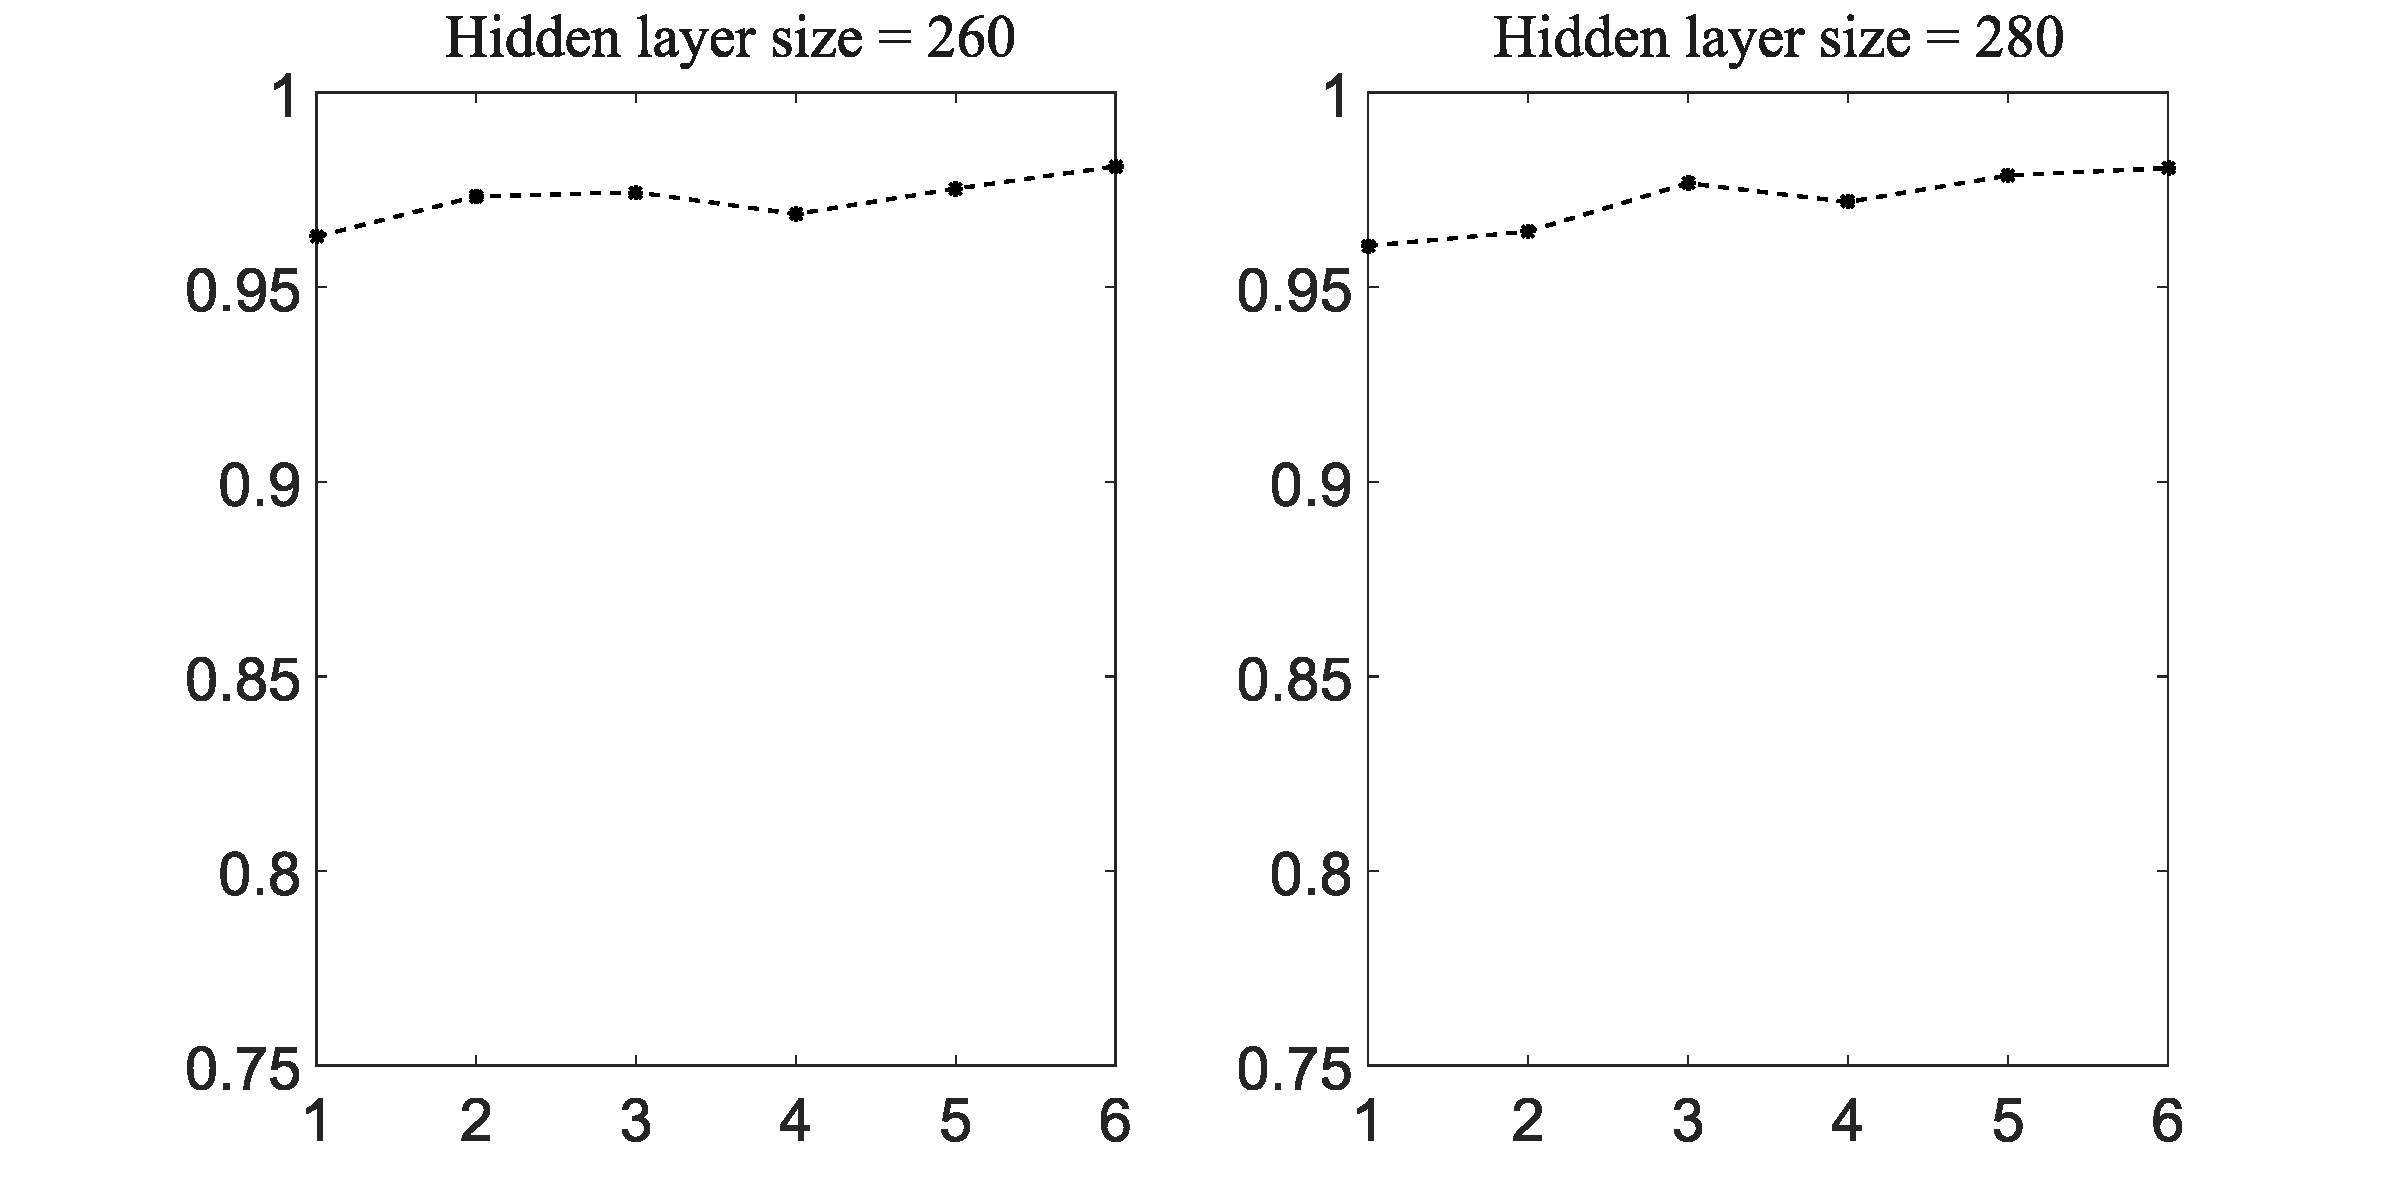
\includegraphics[width=10cm]{AccuracyTSSizeG.pdf}
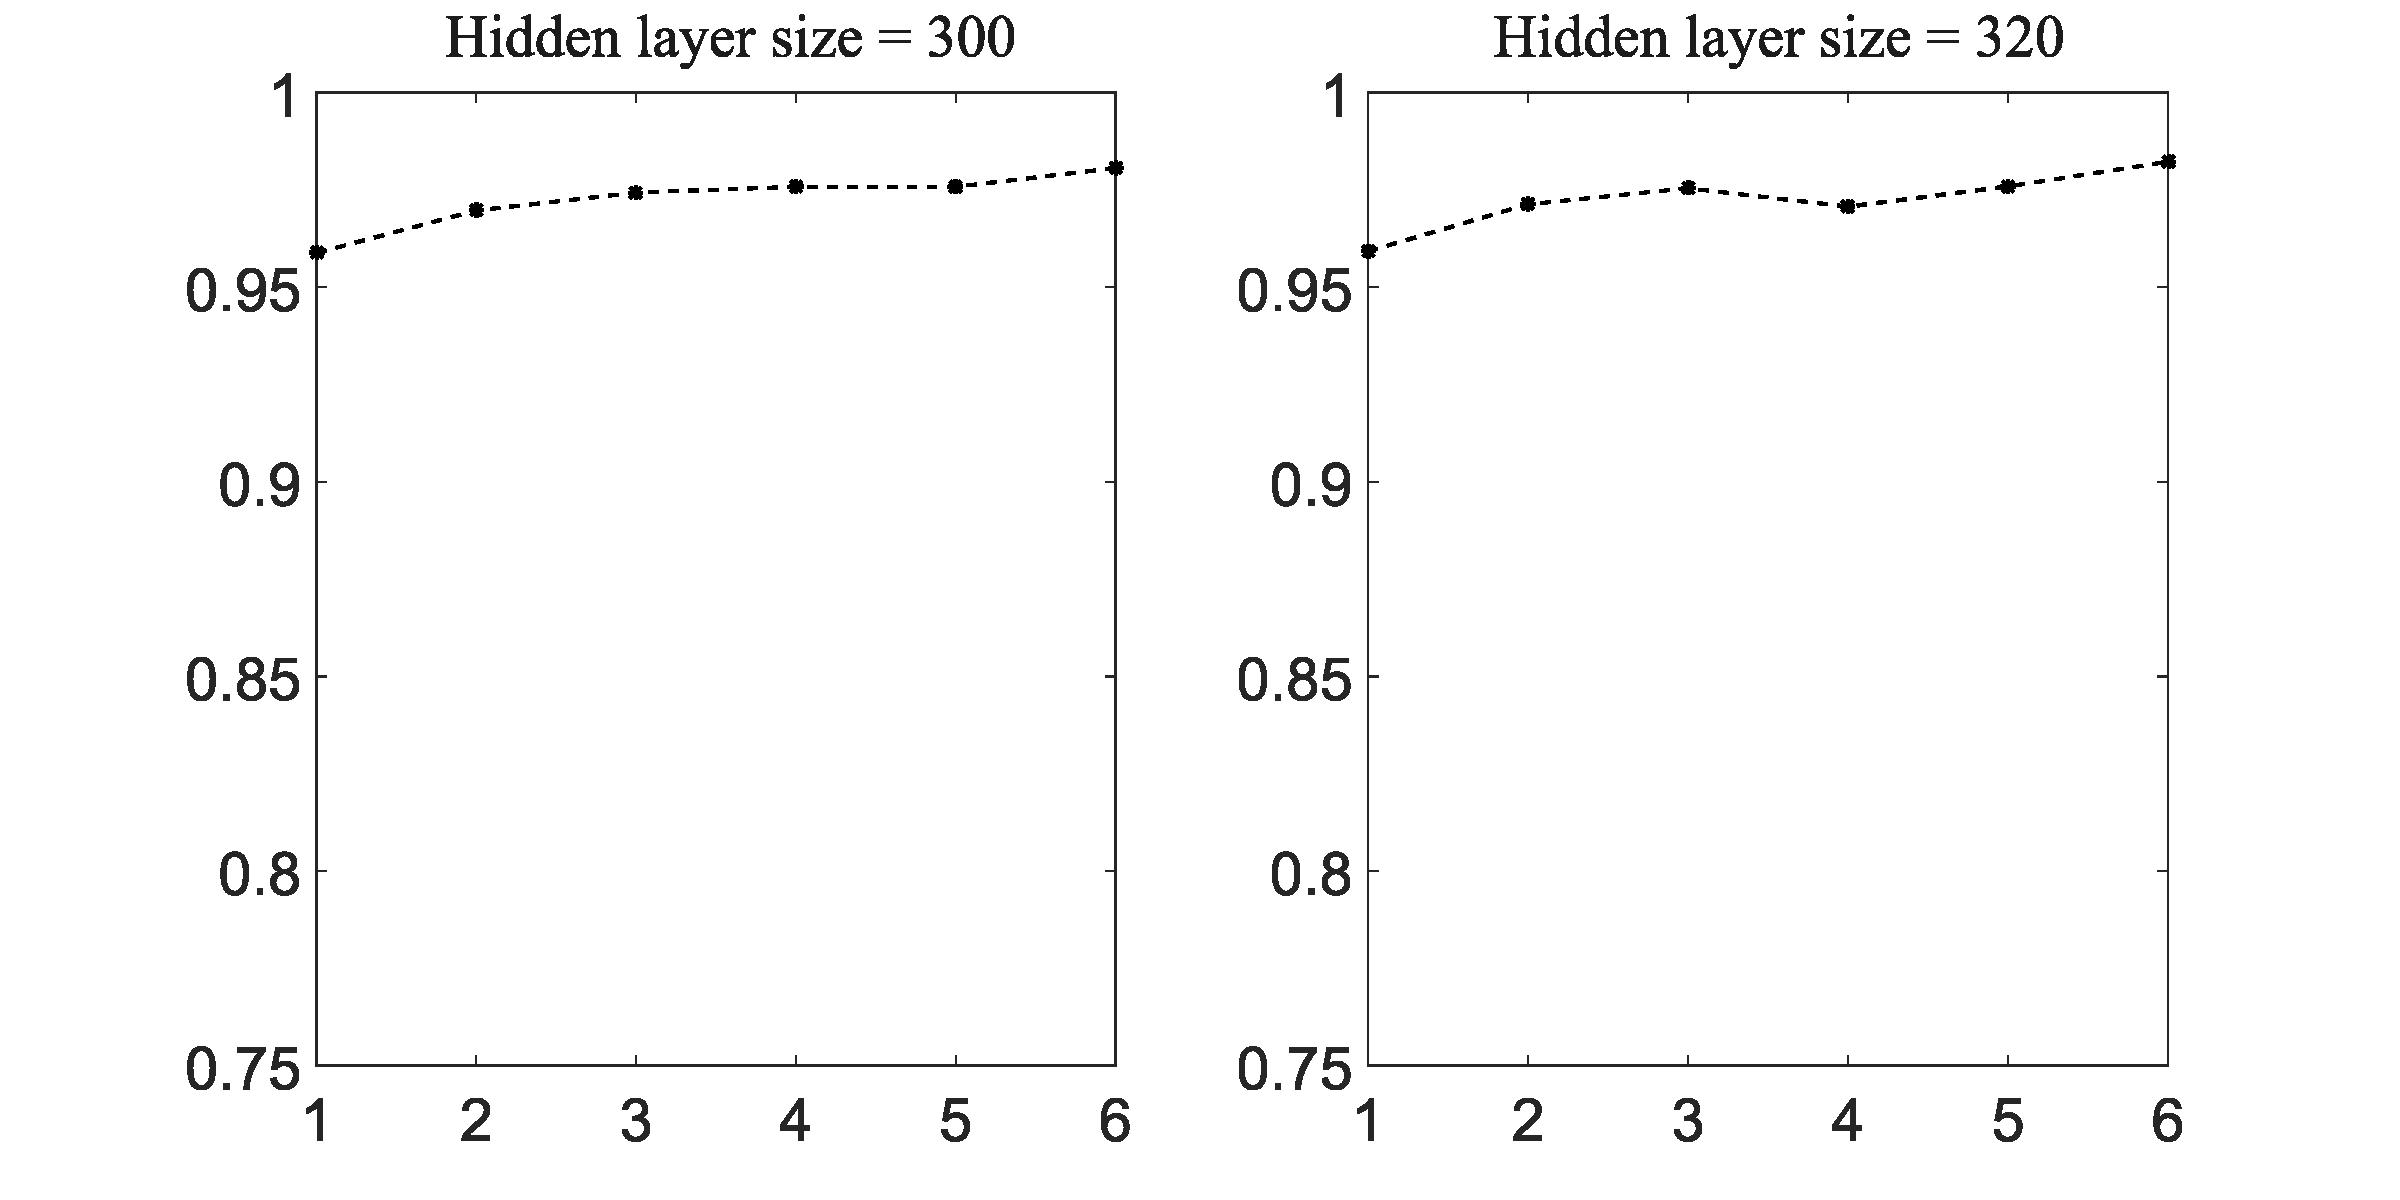
\includegraphics[width=10cm]{AccuracyTSSizeH.pdf}
\caption{Accuracy vs. Training set size}
\label{figure:ATSS_B}
\end{figure}

\begin{figure}[tmbh]
\centering
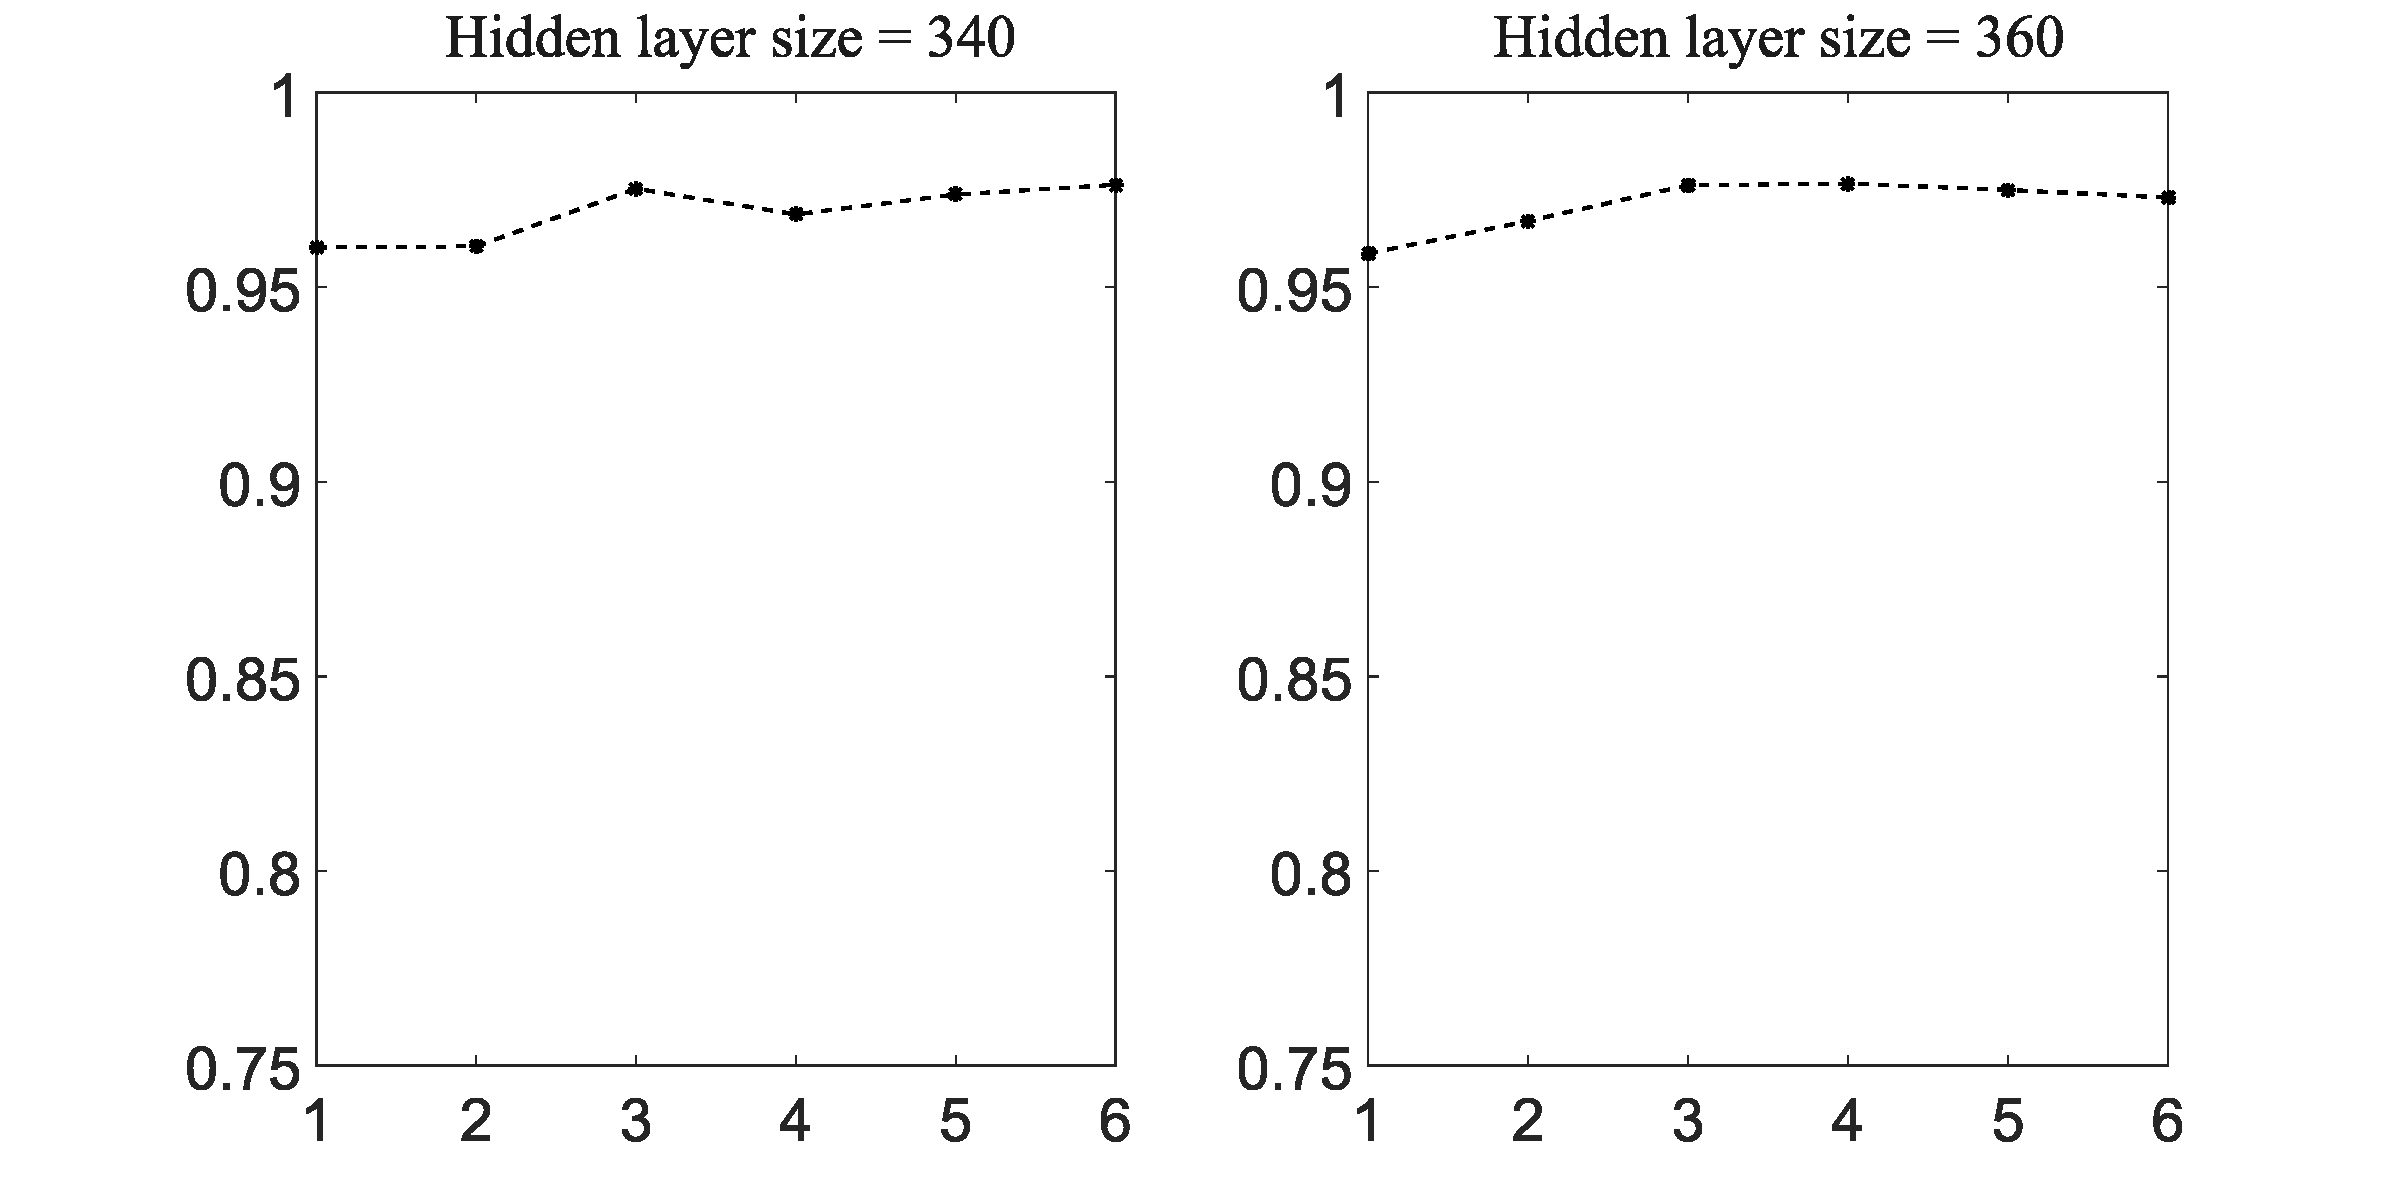
\includegraphics[width=10cm]{AccuracyTSSizeI.pdf}
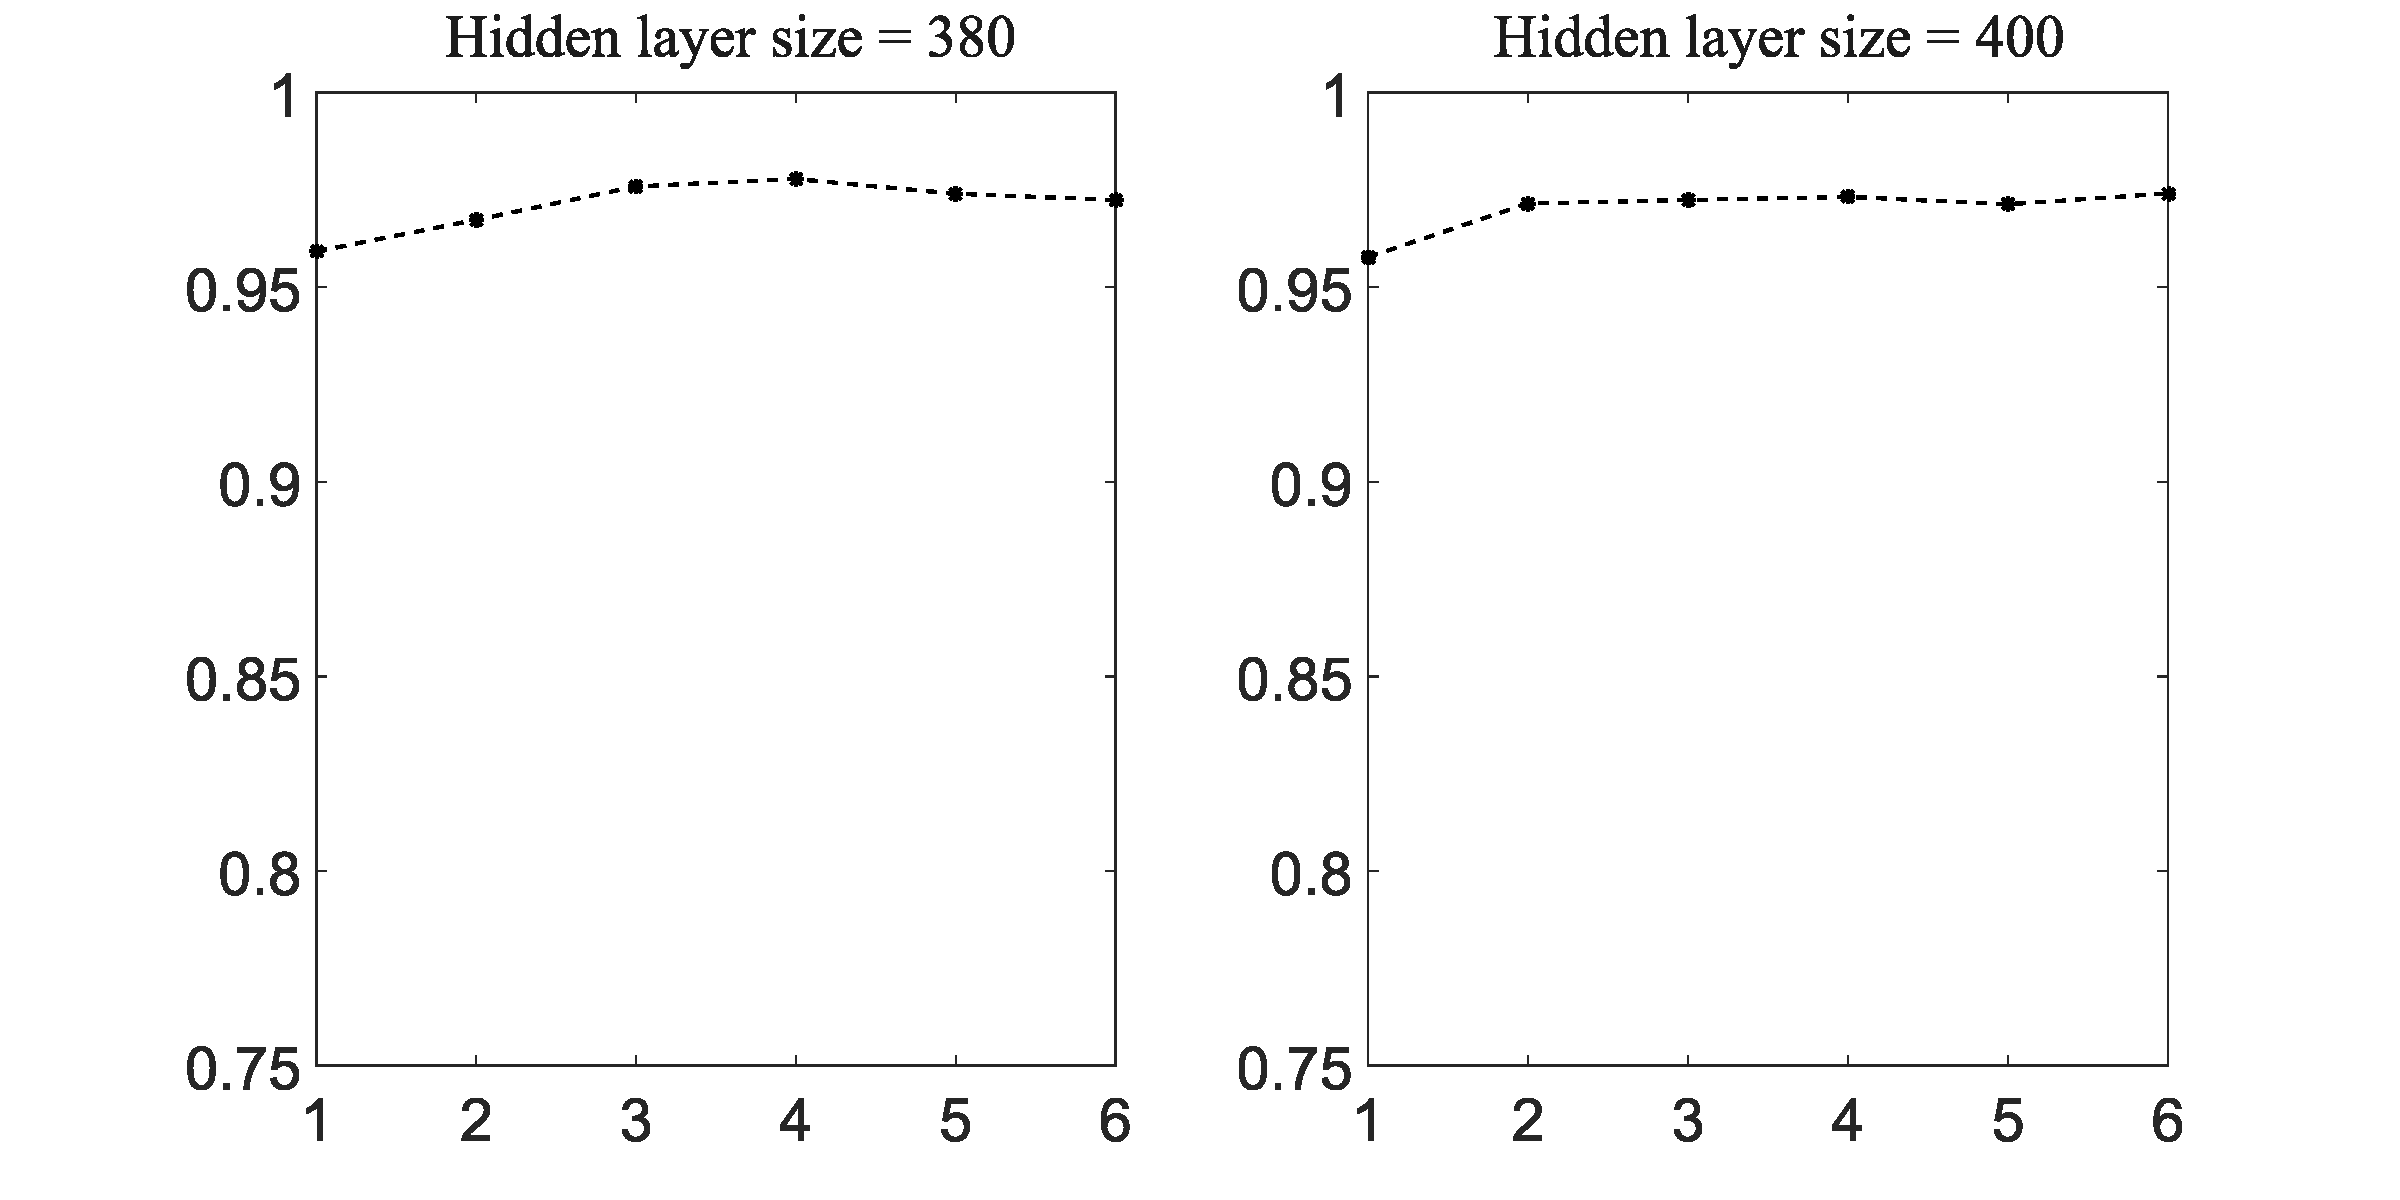
\includegraphics[width=10cm]{AccuracyTSSizeJ.pdf}
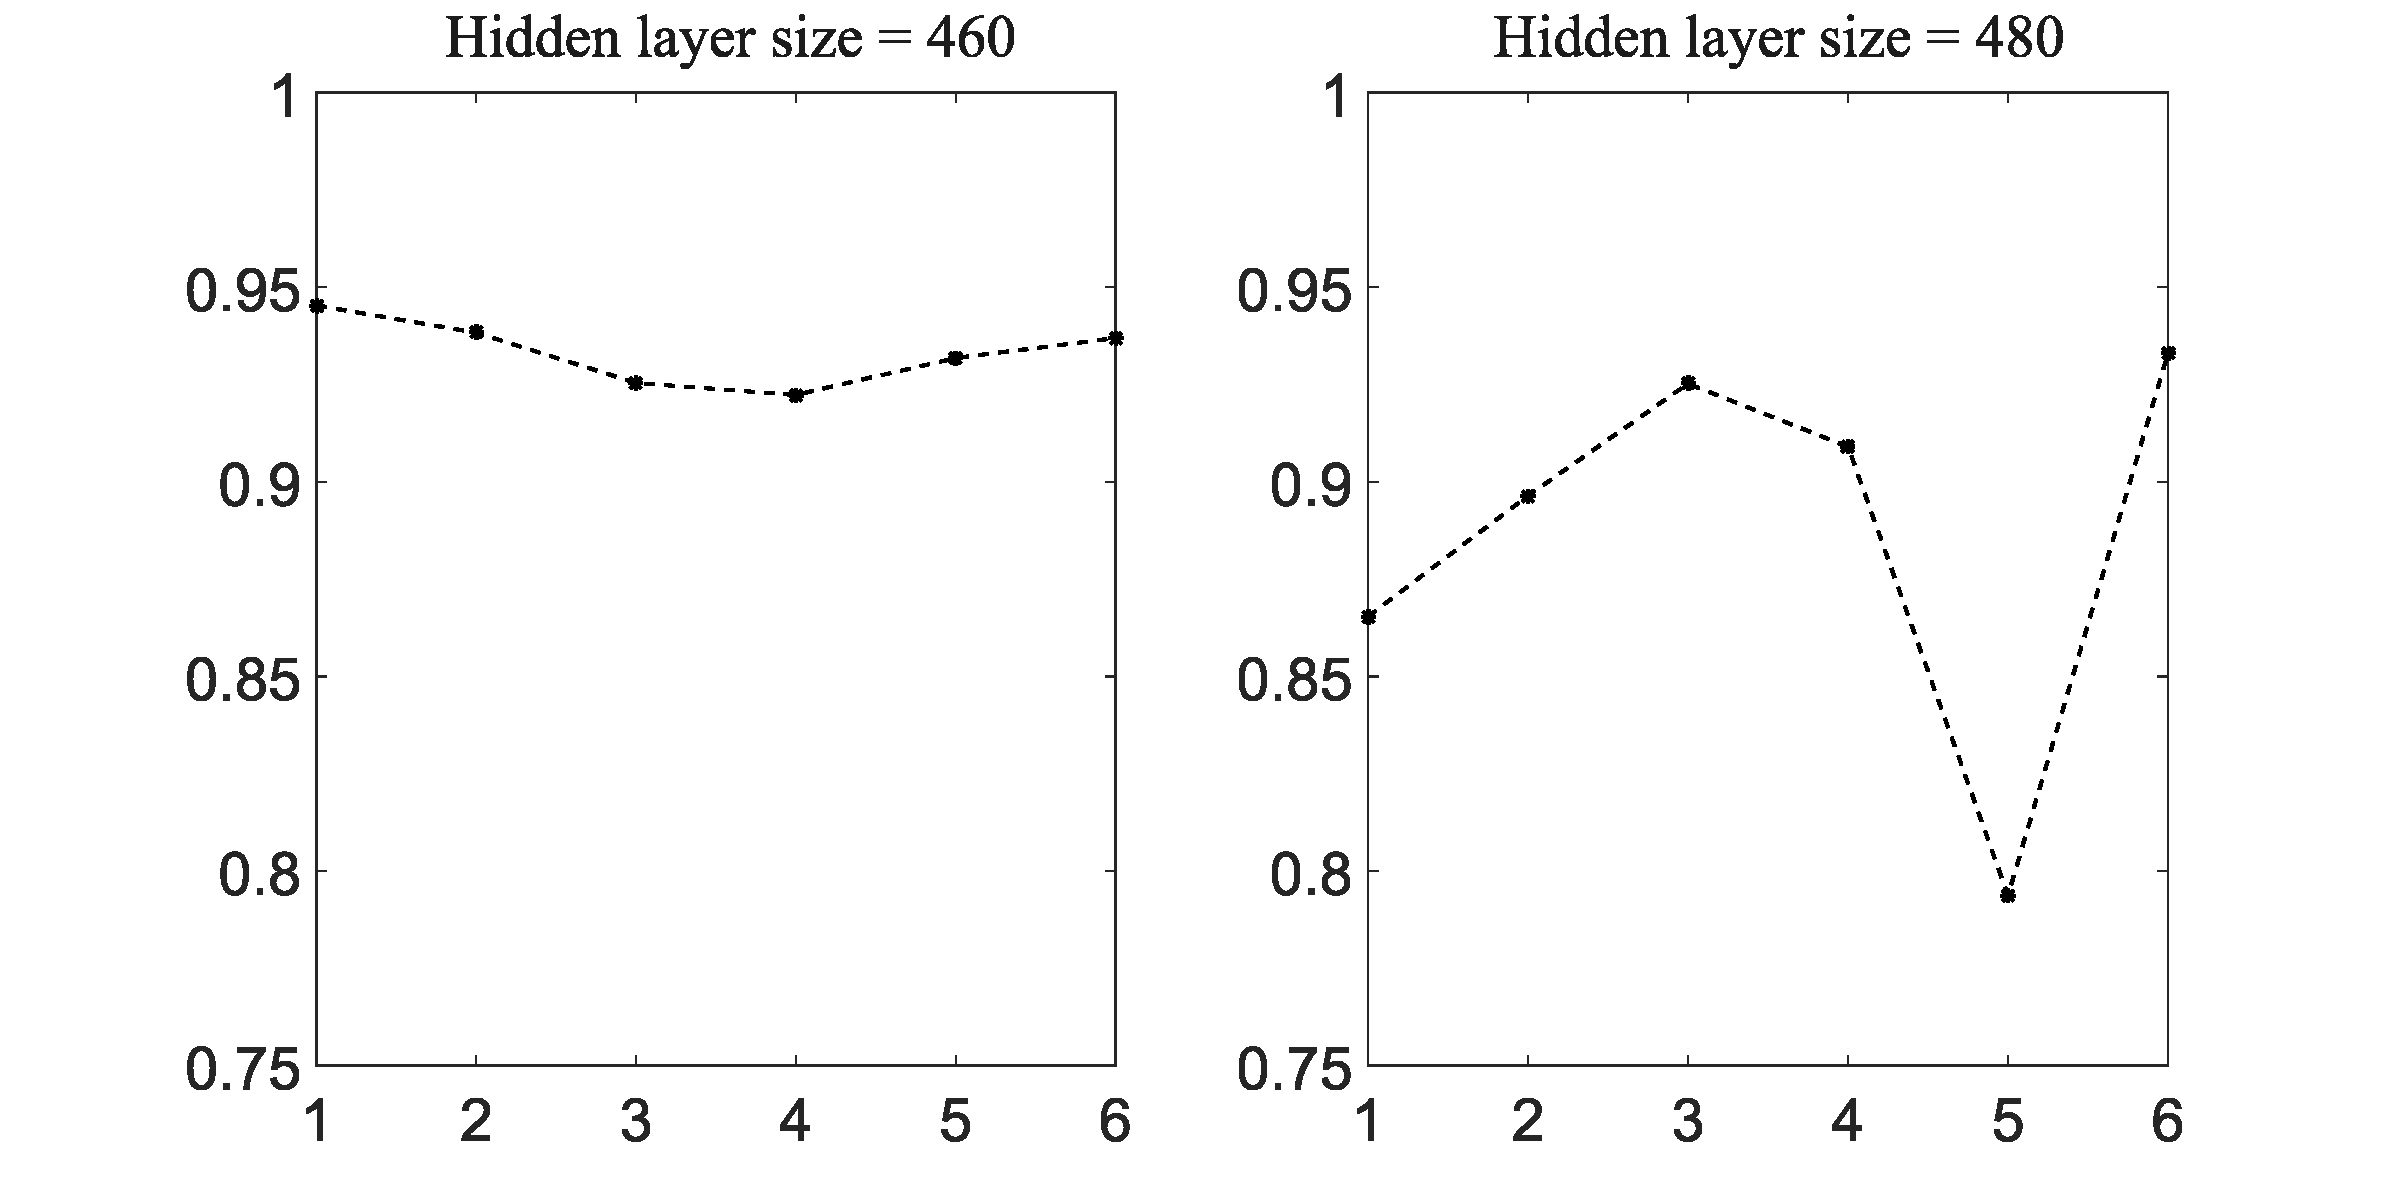
\includegraphics[width=10cm]{AccuracyTSSizeL.pdf}
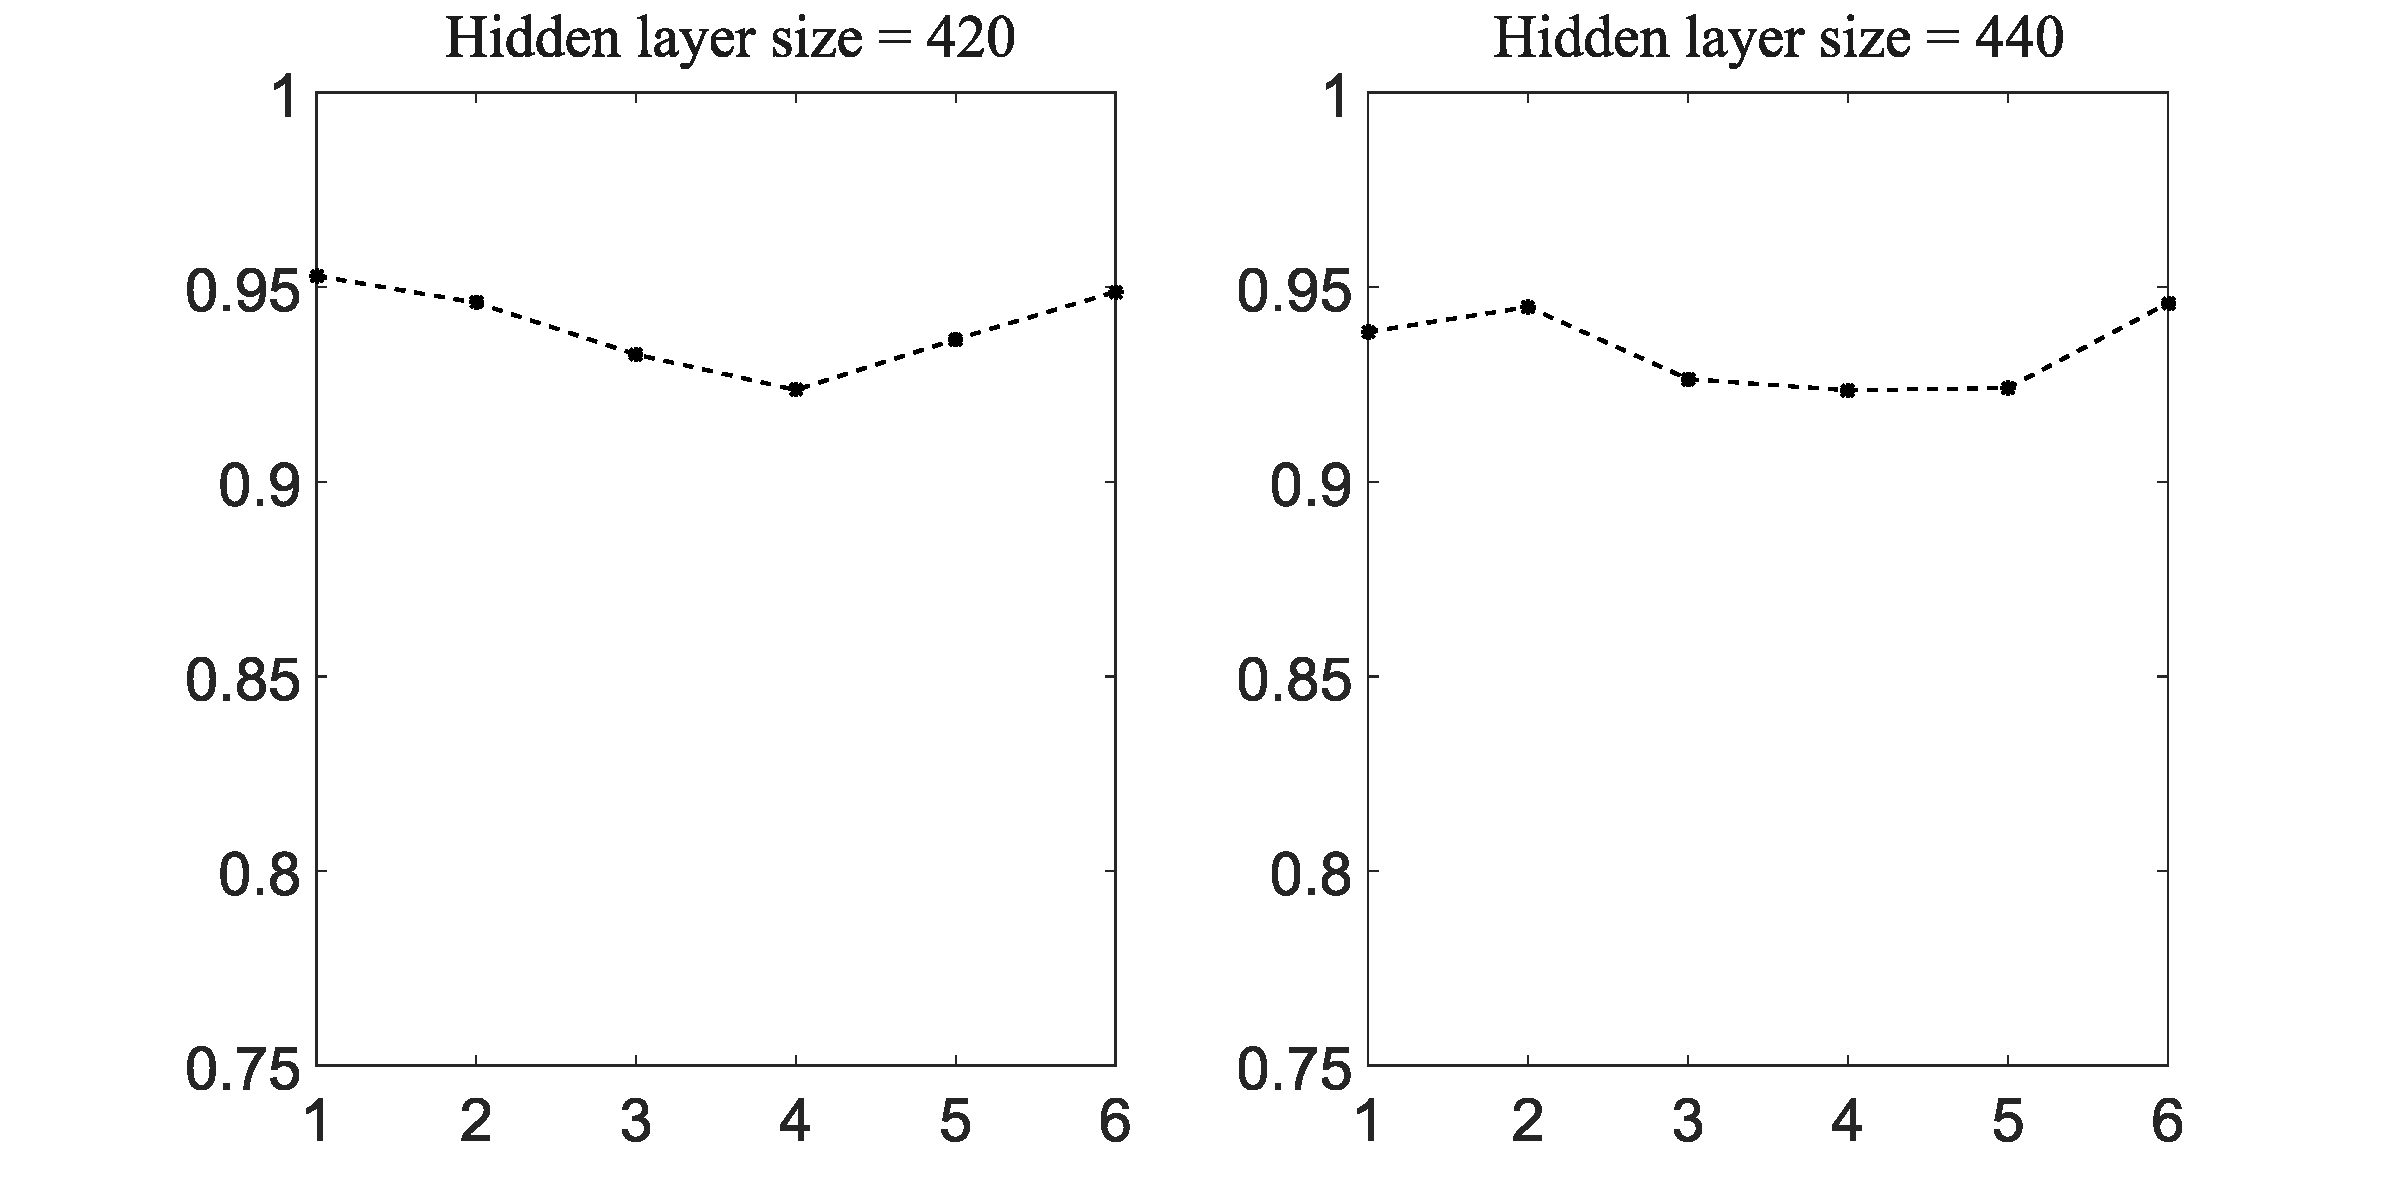
\includegraphics[width=10cm]{AccuracyTSSizeK.pdf}
\caption{Accuracy vs. Training set size}
\label{figure:ATSS_C}
\end{figure}
\end{subfigures}

\end{document}}